%!TEX TS-program = xelatex
%!TEX encoding = UTF-8 Unicode

\documentclass[a4paper,11pt,oneside]{book}
\usepackage{upatras-thesis}

\setmainfont[BoldItalicFont={GFSDidotBoldItalic}, BoldFont={GFSDidotBold}, ItalicFont={GFSDidotItalic}]{GFSDidot.otf}

%
% These commands need to be defined in order to produce a correct and personalized document
%
\newcommand{\shortdoctitle}{Διπλωματική Εργασία}
\newcommand{\doctitle}{Εντοπισμός αλληλεπιδράσεων πρωτεϊνών μέσω συμπλήρωσης μητρώων και αλγορίθμων βαθιάς μάθησης}
\newcommand{\docsubtitle}{Υπότιτλος εγγράφου}
\newcommand{\division}{Ηλεκτρονικής και Υπολογιστών}
\newcommand{\lab}{Multi-Dimensional Data Analysis and Knowledge Management}

\newcommand{\me}{Μηνά Χαμαμτζόγλου του Ιωακείμ} %ΠΡΟΣΟΧΗ: στοιχεία σε γενική πτώση. Παράδειγμα: Άγγελου Σικελιανού του Ιωάννη
%
\newcommand{\nomme}{Μηνάς Χαμαμτζόγλου του Ιωακείμ} %ΠΡΟΣΟΧΗ: στοιχεία σε ονομαστική πτώση. Παράδειγμα: Άγγελος Σικελιανός του Ιωάννη
%
\newcommand{\studnum}{1020700}
\newcommand{\keywords}{keyword1, keyword2, keyword3}
\newcommand{\monthyear}{Ιούνιος 2020}

\newcommand{\supname}{Βασίλειος Μεγαλοοικονόμου}
\newcommand{\suptitle}{Καθηγητής}
\newcommand{\headofdivision}{Βασίλειος Παλιουράς}
\newcommand{\headofdivisiontitle}{Καθηγητής}

\author{\me}

% PDF settings
%
\hypersetup
{
    pdfauthor={\me},
    pdftitle={\shortdoctitle},
    pdfsubject={\doctitle},
    pdfkeywords={\keywords},
    pdfproducer={XeLaTex},
    pdfcreator={\creator}
}

\begin{document}


\pagenumbering{roman}
%set the number of sectioning levels that get number and appear in the contents
\setcounter{page}{3}

\include{titlepage}
\clearemptydoublepage

\include{certification}
\clearemptydoublepage

\pagestyle{empty}
\begin{center}
\Large{Στοιχεία διπλωματικής εργασίας}\\[1cm]
{\large Θέμα:}
\textbf{\large \doctitle}\\[1cm]
\large {Φοιτητής: \textbf{\nomme}\\[1cm]
\large{Ομάδα επίβλεψης}\\
\textbf{\suptitle \, \supname}\\
\textbf{ }\\
\textbf{Διδακτορικός Θωμάς Παπαστεργίου}\\[1cm]
Εργαστήριο\\
\lab \\[1cm]
Περίοδος εκπόνησης της εργασίας:\\ Νοέμβριος 2019 - Ιούνιος 2020\\[1cm]
Η εργασία αυτή γράφτηκε στο \XeLaTeX{} και χρησιμοποιήθηκε η γραμματοσειρά GFS Didot του Greek Font Society.}
\end{center}
\clearemptydoublepage

\pagestyle{plain}
\begin{center}
{\LARGE Περίληψη}\\[1cm]
\end{center}

Αντικείμενο της παρούσας διπλωματικής εργασίας είναι η μελέτη και η κατανόηση των πρωτεϊνικών αλληλεπιδράσεων (Protein Protein Interactions - PPIs ), καθώς και η δημιουργία μοντέλων μηχανικής μάθησης (machine learning models) για τον εντοπισμό των PPIs. 

\medskip
H αλληλεπίδραση μεταξύ πρωτεϊνών αποτελεί ένα αντικείμενο μεγάλης σημασίας για την κατανόηση της λειτουργίας των πρωτεϊνών και έναν από τους βασικούς στόχους της συστημικής βιολογίας (systems biology ) \cite{Rao2014}. Αφού πρώτα παρουσιαστεί το θεωρητικό βιολογικό υπόβαθρο της εργασίας, γίνεται αναφορά στους τρόπους εντοπισμού των εν λόγω αλληλεπιδράσεων, τόσο πειραματικά όσο και υπολογιστικά, ενώ το κεφάλαιο ολοκληρώνεται με την επιγραμματική αναφορά στις μεγαλύτερες βάσεις δεδομένων πρωτεϊνικών αλληλεπιδράσεων.

\medskip
Το δεύτερο μέρος της εργασίας αφορά την εισαγωγή στις βασικές έννοιες της μηχανικής μάθησης. Με τον όρο \textit{μηχανική μάθηση} αναφερόμαστε σε μεθόδους ανάλυσης και επεξεργασίας δεδομένων με σκοπό την αυτοματοποίηση μοντέλων μηχανών και υπολογιστικών συστημάτων. Δίνονται ορισμοί και αναπτύσσονται έννοιες όπως τα νευρωνικά δίκτυα που θα αναπτυχθούν λεπτομερώς και στην υλοποίηση της εργασίας.

\medskip
Έπειτα από την ολοκλήρωση του θεωρητικού πλαισίου της εργασίας, υλοποιείται η προσέγγιση της παρούσας διπλωματικής. Ξεκινάει με τον ορισμό του προβλήματος και την ανάλυση της εξαγωγής δεδομένων αλληλεπιδράσεων πρωτεϊνών. Έπειτα από τη δημιουργία του συνόλου δεδομένων, παρουσιάζονται τεχνικές \textit{συμπλήρωσης μητρώων} (\textit{matrix completion}), μαθηματικές μέθοδοι συμπλήρωσης μη-υπαρχόντων τιμών στο σύνολο των δεδομένων, με σκοπό την μείωση της διαστασιμότητας του προβλήματος και την βελτίωση της απόδοσης των αλγορίθμων μας. Παρουσιάζεται μια τεχνική παραγοντοποίησης μητρώου μέσω stochastic gradient descent (matrix factorization with SGD), καθώς και μια τεχνική τανηστικής αποδόμησης (tensor decomposition). Έπειτα από την επεξεργασία των δεδομένων ακολουθεί η ανάπτυξη νευρωνικών δικτύων για τον εντοπισμό αλληλεπιδράσεων. Παρουσιάζονται λεπτομερώς οι αρχιτεκτονικές που χρησιμοποιήθηκαν στα πλαίσα της εργασίας, ενώ συγκρίνεται η απόδοση των εν λόγω δομών με υπάρχοντα μοντέλα. Η εργασία ολοκληρώνεται με την παρουσίαση των μελλοντικών σκέψεων σχετικά με την εξέλιξη των μοντέλων και την βελτίωση των αποτελεσμάτων.

\medskip
\noindent{\large\textbf{Λέξεις-Κλειδιά:}} Πρωτεΐνες, αλληλεπιδράσεις πρωτεϊνών, συμπλήρωση μητρώου, παραγοντοποίηση μητρώου, τανυστική αποδόμηση, μηχανική μάθηση, νευρωνικά δίκτυα.



\clearemptydoublepage

\begin{center}
{\LARGE Ευχαριστίες}\\[1cm]
\end{center}

Αρχικά, θα ήθελα να ευχαριστήσω τον επιβλέποντα καθηγητή της διπλωματικής μου εργασίας κ. Βασίλειο Μεγαλοοικονόμου για την εμπιστοσύνη που μου έδειξε καθ' όλη τη διάρκεια εκπόνησης της εργασίας αλλά και την πολύτιμη καθοδήγησή του. 

\medskip
Στη συνέχεια, ευχαριστώ ιδιαιτέρως τον διδάκτορα Θωμά Παπαστεργίου για τις πολύτιμες συμβουλές αλλά και τις υποδείξεις του σχετικά με την κατεύθυνση της εργασίας, καθώς χωρίς αυτές η συγκεκριμένη εργασία δεν θα μπορούσε να ολοκληρωθεί. Παράλληλα, θα ήθελα να ευχαριστήσω όλα τα παιδιά του εργαστηρίου Multi-Dimensional Data Analysis and Knowledge Management για το όμορφο κλίμα και την ενθάρρυνση σε όλη την πορεία αυτής της εργασίας.

\medskip
Εξαιρετικά ευγνώμων είμαι προς την οικογένειά μου, η οποία στήριξε όλες μου τις επιλογές και για τις θυσίες τους προκειμένου να ολοκληρώσω τις σπουδές μου.

\medskip
Ευχαριστώ ιδιαίτερα τον Παναγιώτη και τον Βασίλη για τις όμορφες και εποικοδομητικές κουβέντες, προσφέροντάς μου συνεχώς νεα ερεθίσματα και βοηθώντας με να δω την εργασία με νεα οπτική. Τέλος, θα ήθελα να ευχαριστήσω όλους τους κοντινούς μου ανθρώπους, που στάθηκαν δίπλα μου τόσο στις εύκολες όσο και στις δύσκολες στιγμές. 

\clearemptydoublepage

\pagestyle{fancy}

\tableofcontents
\listoffigures
\listoftables
%\mainmatter % book mode only
\clearemptydoublepage

\pagenumbering{arabic}
\setcounter{page}{1}

%!TEX root = ../main.tex

\chapter*{Εισαγωγή}
\markboth{Εισαγωγη}{}
%\vspace{-1.3in}

Οι πρωτεΐνες αποτελούν μια κατηγορία μακρομορίων που ελέγχει όλες τις βιολογικές διαδικασίες μέσα σε ένα κύταρρο και είναι άρρηκτα συνδεδεμένες με την υγεία των ανθρώπων. Παρ' ότι αρκετές πραγματοποιούν τις διεργασίες τους ως ανεξάρτητες οντότητες, η πλειοψηφία των πρωτεϊνών αλληλεπιδρά με άλλες πρωτεΐνες για την ορθή βιολογική δραστηριότητα. Επομένως, για την καλύτερη κατανόηση της λειτουργίας των πρωτεϊνών και συνεπώς και των οργανισμών, είναι σημαντικό ζήτημα ο εντοπισμός και η μελέτη των αλληλεπιδράσεων μεταξύ των πρωτεϊνών (γνωστές και ως \textit{Protein Protein Interractions - PPI}). Αν και στη θεωρία φαίνεται ως μια απλή διαδικασία, πρακτικά αποτελεί ένα εξαιρετικά δύσκολο ζήτημα, διότι τα κύταρρα αντιδρούν σε μια πληθώρα ερεθισμάτων, καθιστώντας την έκφραση των πρωτεϊνικών διεργασιών μια δυναμική διαδικασία με πολλαπλές παραμέτρους. Παράλληλα, οι πρωτεΐνες που συμμετέχουν σε μια αλληλεπίδραση μπορεί να μην είναι πάντα ενεργοποιημένες ή εμφανείς (στην πραγματικότητα οι περισσότερες αλληλεπιδράσεις είναι προσωρινού χαρακτήρα και απαιτούν έναν αριθμό συνθηκών για να πραγματοποιηθούν). 

\medskip
Οι ίδιες οι αλληλεπιδράσεις αποτελούνται από εναν συνδυασμό υδροφοβικών δεσμών με δυνάμεις \textit{Van der Waals} και \textit{γέφυρες αλάτων} (\textit{salt bridges}) σε συγκεκριμένες περιοχές (\textit{binding domains}) σε κάθε πρωτεΐνη. Ο εντοπισμός τους γίνεται εργαστηριακά μέσω μιας σειράς βιοχημικών πειραμάτων, τόσο \textit{in vivo} οσο και \textit{in vitro} (π.χ. co-immunoprecipation, TAP tagging, X-ray crystallography, Yeast two-hybrid κ.α.). Ωστόσο, ο τεράστιος αριθμός πιθανών αλληλεπιδράσεων σε συνδυασμό με το μεγάλο κόστος των παραπάνω πειραμάτων καθιστά αναγκαία τη δημιουργία αυτοματοποιημένων προσεγγίσεων για τον εντοπισμό ή/και την πρόβλεψη αλληλεπιδράσεων. Οι προσεγγίσεις αυτές, εκτελεσμένες σε υπολογιστή ή μέσω υπολογιστικής προσωμοίωσης, ονομάζονται μέθοδοι \textit{in silico} και αποτελούν κομμάτι της βιοπληροφορικής (\textit{bioinformatics}), τομέα που αφορά την κατασκευή μεθόδων και εργαλείων λογισμικού για την κατανόηση και επεξεργασία βιολογικών δεδομένων. Η συγκεκριμένη εργασία ασχολείται με δομικές προσεγγίσεις in silico τεχνικών, οπου προβλέπεται αλληλεπίδραση μεταξύ δυο πρωτεϊνών με βάση τα δομικά τους χαρακτηριστικά. Ειδικότερα, ασχολείται με τη δημιουργία μοντέλων μηχανικής μάθησης για την πρόβλεψη αλληλεπιδράσεων μεταξύ πρωτεϊνών.

\medskip
Η αύξηση της υπολογιστικής ισχύος έχει οδηγήσει τα τελευταία χρόνια στην ραγδαία ανάπτυξη του αντικειμένου της μηχανικής μάθησης, με τα μοντέλα μηχανικής μάθησης να αποδίδουν εξαιρετικά σε πολλούς τομείς όπως η υγεία, η βιολογία, τα οικονομικά κ.α. Στον τομέα της βιοπληροφορικής, η μηχανική μάθηση εφαρμόζεται σε τομείς τομείς όπως η \textit{γονιδιωματική} (\textit{genomics}), η \textit{εξέλιξη} (\textit{evolution}) και η βιολογία συστημάτων (\textit{systems biology}). Πλεόν, ο μεγάλος αριθμός βιολογικών δεδομένων δεν αποτελεί ανασταλτικό παράγοντα, αλλά το ερώτημα μετατοπίζεται στην κατανόηση του τεράστιου όγκου πληροφορίας και στην αξιοποίησή του. Ακολουθίες, δισδιάστατες και τρισδιάστατες δομές, καθώς και δίκτυα αλληλεπιδράσεων αποτελούν μόνο μερικά από τα δεδομένα ενδιαφέροντος. Όσον αφορά την πρόβλεψη αλληλεπιδράσεων πρωτεϊνών, η μηχανική μάθηση φαίνεται να έχει εξαιρετικά αποτελέσματα (Support Vector Machines \cite{Bradford2005}, Random Forests \cite{Mengying2017}, Convolutional Neural Networks \cite{Xie2020}, Bayesian networks \cite{NEUVIRTH2004} etc ).

\medskip
Στην διπλωματική εργασία κατασκευάστηκαν νευρωνικά δίκτυα με σκοπό την πρόβλεψη αλληλεπιδράσεων μεταξύ πρωτεϊνών, ωστόσο ακολουθήθηκε μια νεα προσέγγιση όσον αφορά την επεξεργασία των δεδομένων. Ειδικότερα, εφαρμόστηκαν μέθοδοι συμπλήρωσης μητρώων (\textit{matrix completion}), οπου συμπληρώθηκαν οι ελλιπείς τιμές των δεδομένων με βάση τις υπόλοιπες παρατηρίσιμες τιμές. Οι τεχνικές αυτές αποτελούν μια μορφή συνεργατικού φιλτραρίσματος (\textit{collaborative filtering}), κατά την οποία επιχειρούμε να εξάγουμε πληροφορία ή μοτίβα για τη συμπλήρωση τιμών συμπεριλαμβάνοντας πληροφορίες από πολλαπλές εγγραφές \cite{Terveen2001}. Οι μέθοδοι που χρησιμοποιήθηκαν ήταν η \textit{παραγοντοποίηση μητρώου μέσω Stochastic Gradient Descent} (\textit{Matrix Factorization with SGD}) και η \textit{τανηστική αποδόμηση CP} ( \textit{CP Tensor Decomposition}), για τις οποίες γίνεται λεπτομερής ανάλυση στη συνέχεια.

\medskip
Επειτα από την επεξεργασία των δεδομένων, εκπαιδεύτηκαν μοντέλα νευρωνικών δικτύων, και συγκεκριμένα ένα πλήρως διασυνδεδεμένο νευρωνικό δίκτυο (\textit{fully connected neural network}) και ένα συνελικτικό νευρωνικό δίκτυο (\textit{convolutional neural network}), ενώ αξιολογήθηκε η απόδοση τους σε σύγκριση με αντίστοιχες δημοσιευμένες εργασίες. Οι μετρικές που χρησιμοποιήθηκαν για την αξιολόγηση των μοντέλων ήταν: Accuracy, Precision, Sensitivity, Specificity, F-score και Matthews Correlation Co\-efficient (MCC). 




\clearemptydoublepage

\chapter{Πρωτεΐνες}\label{ch:chap1}
%!TEX root = ../main.tex

\setcounter{secnumdepth}{4}

\titleformat{\paragraph}
{\normalfont\normalsize\bfseries}{\theparagraph}{1em}{}
\titlespacing*{\paragraph}
{0pt}{3.25ex plus 1ex minus .2ex}{1.5ex plus .2ex}

Στο κεφάλαιο αυτό παρουσιάζεται η θεωρία γύρω από το αντικείμενο των πρωτεΐνών και των πρωτεϊνικών αλληλεπιδράσεων (γνωστές ως Protein - Protein Interactions). Αρχικά, δίνεται ένας σύντομος ορισμός των πρωτεϊνών, που αποτελούν τα δομικά και λειτουργικά στοιχεία των οργανισμών. Στη συνέχεια, γίνεται μια εισαγωγή στο αντικείμενο των PPIs και αναφέρονται οι κατηγορίες αλληλεπιδράσεων. Έπειτα, αναπτύσσονται οι μέθοδοι εντοπισμού αλληλεπιδράσεων πρωτεϊνών τόσο σε πειραματικό στάδιο όσο και υπολογιστικά με τη βοήθεια υπολογιστών. Το κεφάλαιο κλείνει με μια σύντομη αναφορά στις βάσεις δεδομένων που έχουν δημιουργηθεί για την καταγραφή, αποθήκευση και ανάλυση των πρωτεϊνικών αλληλεπιδράσεων.

\section{Ορισμός, Λειτουργίες}

Οι πρωτεΐνες αποτελούν μεγάλα και πολύπλοκα μόρια που παίζουν καθοριστικό ρόλο στις διαδικασίες λειτουργίας και αναπαραγωγής ενός οργανισμού \cite{Stephenson2016}.Στην πρωτοταγή δομή τους, αποτελούνται από μια ή περισσότερες αλυσίδες αμινοξέων (amino acid residues). Αμινοξέα ονομάζονται τα μόρια που αποτελούνται από 3 χημικές ομάδες και ένα άτομο υδρογόνου τα οποία συνδέονται μέσω ομοιοπολικών δεσμών με το ίδιο άτομο άνθρακα. Οι 3 αυτές χημικές ομάδες είναι:
\begin{enumerate}
    \item μια καρβονική ομάδα  \ce{RCOOH} 
    \item μια αμινομάδα \ce{NH2} και
    \item μια πλευρική αλυσίδα μεταβλητού μεγέθους (συμβολίζεται ως \ce{R} )
\end{enumerate}

\medskip
Υπάρχουν 20 διαφορετικοί τύποι αμινοξέων που μπορούν να συνδυαστούν για τη δημιουργία πρωτεϊνών. Η αλληλουχία των αμινοξέων καθορίζει την 3-D δομή της πρωτεΐνης καθώς και τη 
λειτουργία της \cite{Blanco2017}.

\begin{figure}[h]
  \centering
  \includegraphics[scale=0.75]{images/AAS.jpg}
  \caption{Δομή ενός αμινοξέος}
  \label{fig:AAS}
\end{figure}


Η δευτεροταγής δομή των πρωτεΐνών αφορά τη γενικότερη 3-D αρχιτεκτονική των τοπικών στοιχείων της. Οι συνηθέστερες δευτερογενής δομές είναι:
\begin{enumerate}
    \item η "α-έλικα" δεξιόστροφη (a-helix) και
    \item η "β-πτυχωτή επιφάνεια" (b-sheets)
\end{enumerate}

\begin{figure}[h]
  \centering
  \includegraphics[scale=0.35]{images/sec_str.jpg}
  \caption{Δευτερογενής δομή πρωτεΐνών}
  \label{fig:sec_str}
\end{figure}
Όσον αφορά τις λειτουργίες των πρωτεϊνών, αυτές συναντώνται σε όλες τις διαστάσεις της κυτταρικής ζωής. Ορισμένες από αυτές παρουσιάζονται στον παρακάτω πίνακα:

\begingroup
\centering
\begin{tabularx}{1\textwidth} { 
  | >{\raggedright\arraybackslash}X 
  | >{\centering\arraybackslash}X 
  | >{\raggedleft\arraybackslash}X | }
  \hline
 \multicolumn{2}{|c|}{Λειτουργίες Πρωτεϊνών} \\
 \hline
 \textbf{Λειτουργία} & \textbf{Περιγραφή}\\
 \hline
 Άμυνα  & Πρωτεΐνες, όπως τα αντισώματα, δένονται πάνω σε άγνωστα σωματίδια (π.χ. ιοί, βακτήρια, προκειμένου να προστατεύσουν τον οργανισμό \\
\hline
Ένζυμο & Τα ένζυμα υλοποιούν σχεδόν όλες τις χημικές αντιδράσεις των κυττάρων. Ταυτόχρονα βοηθούν στη δημιουργία νέων μορίων διαβάζοντας τη γενετική πληροφορία που βρίσκεται αποθηκευμένη στο DNA.\\
\hline
Μεταφορά & Διάφορες πρωτεΐνες, όπως κάποια είδη ορμονών, μεταδίδουν σήματα για να συντονίσουν βιολογικές διεργασίες μεταξύ διαφορετικών κυττάρων, ιστών ή/και οργάνων. \\
\hline
Δομικό Στοιχείο & Παρέχουν δομή και στήριξη στα κύτταρα. Μακροσκοπικά, επιτρέπουν την κίνηση του οργανισμού. \\
\hline
Αποθήκευση & Δένουν και μεταφέρουν άτομα και μικρομόρια δια μέσω των κυττάρων σε όλο τον οργανισμο \\
\hline
\end{tabularx}
\captionof{table}{Λειτουργίες πρωτεϊνών}\label{Λειτουργίες πρωτεϊνών}
\endgroup


\section{Αλληλεπίδραση πρωτεΐνης με πρωτεΐνη}

Για να εκτελέσουν τις λειτουργίες τους μέσα στα κύτταρα, οι πρωτεΐνες σπανίως λειτουργούν ως απομονωμένες οντότητες. Αντιθέτως, πάνω από το 80\% των πρωτεϊνών εκτελούν τις λειτουργίες τους σε ομάδες\cite{Yanagida2002}, με την μέση πρωτεΐνη να αλληλεπιδρά με 3 εως 10 άλλες πρωτεΐνες\cite{Northey2017}. Μέσω της δημιουργίας ομάδων, οι πρωτεΐνες χειρίζονται ένα ευρύ φάσμα βιολογικών διεργασιών, μεταξύ των οποίων ο έλεγχος του μεταβολισμού και της ανάπτυξης των κυττάρων και η κυτταρική αλληλεπίδραση\cite{Rao2014}. Επομένως, ένα σημαντικό βήμα για την κατανόηση των μοριακών σχέσεων μεταξύ των οργανισμών είναι η "χαρτογράφηση" των φυσικών αλληλεπιδράσεων πρωτεΐνης με πρωτεΐνη (PPIs). 

\smallskip
Ως αλληλεπίδραση αναφερόμαστε στις συγκεκριμένες φυσικές επαφές μεταξύ ζεύγων πρωτεϊνών που συμβαίνουν μέσω επιλεκτικής μοριακής σύνδεσης σε ένα αυστηρά συγκεκριμένο βιολογικό πλαίσιο \cite{Rivas2010}. Η σύνδεση αυτή προκύπτει από μια πληθώρα βιοχημικών γεγονότων, μεταξύ των οποίων λόγω ηλεκτροστατικών δυνάμεων, δεσμών υδρογόνου και λόγω υδροφοβικότητας. Οι πρωτεΐνες συνδέονται μεταξύ τους μέσω περιοχών τους που είναι τόσο γεωμετρικά όσο και φυσιοχημικά συμπληρωματικές μεταξύ τους, οπότε και προκύπτουν ενεργειακά ευνοϊκές αλληλεπιδράσεις. Στον παρακάτω πίνακα παρουσιάζονται τα είδη των αλληλεπιδράσεων που αναπτύσσουν οι πρωτεΐνες μεταξύ τους:


\medskip
\begingroup
\begin{tabularx}{0.8\textwidth} { 
  | >{\raggedright\arraybackslash}X 
  | >{\centering\arraybackslash}X 
  | >{\raggedleft\arraybackslash}X | }
  \hline
 \multicolumn{3}{|c|}{Τύποι Αλληλεπιδράσεων Πρωτεΐνης με Πρωτεΐνη} \\
 \hline
    Με βάση την αλληλεπίδραση & Ομο-ολιγομερής (Homooligomeric) & Ετερο-ολιγομερής (Heterooligomeric)\\
 \hline
    Με βάση την ευστάθειά τους & Υποχρεωτικές (obligate) & Μη υποχρεωτικές (non obligate) \\
 \hline
    Με βάση το προσδόκιμο ζωής & Εφήμερες (Transient) & Σταθερές (Permanent) \\
 \hline
\end{tabularx}
\captionof{table}{Τύποι Αλληλεπιδράσεων Πρωτεΐνης με Πρωτεΐνη}\label{Τύποι Αλληλεπιδράσεων Πρωτεΐνης με Πρωτεΐνη}
\endgroup

\medskip
Ειδικότερα, \textit{oμοολιγομερείς} ονομάζονται οι αλληλεπιδράσεις μεταξύ ομοίων αλυσίδων ενώ \textit{ετεροολιγομέρεις} αυτές μεταξύ διαφορετικών αλυσίδων. Επιπλέον διαφοροποίηση παρατηρείται όσον αφορά την ευστάθεια των δεσμών,με τις αλληλεπιδράσεις να διακρίνονται σε \textit{υποχρεωτικές}, όπου τα πρωτομερή (δομικές μονάδες ολιγομερών πρωτεϊνών) δεν μπορούν να υπάρξουν ως ευσταθείς δομές \textit{in vivo}, και \textit{μη υποχρεωτικές}. Οι αλληλεπιδράσεις διαφοροποιούνται και όσον αφορά το προσδόκιμο ζωής της σύνδεσης. \textit{Σταθερές} ή \textit{μόνιμες} είναι αλληλεπιδράσεις με υψηλή ευστάθεια και μόνιμο χαρακτήρα, ενώ οι \textit{εφήμερες} αλληλεπιδράσεις αφορούν συνδέσεις και αποσυνδέσεις \textit{in vivo}. Ταυτόχρονα, υπάρχει ένας περαιτέρω διαχωρισμός των εφήμερων αλληλεπιδράσεων σε \textit{αδύναμες} (weak transient), όπου η ισορροπία συνεχώς χάνεται και ανακτάται, και \textit{ισχυρές} (strong transient),όπου απαιτείται κάποια μοριακή διατάραξη για να χαθεί η ισορροπία\cite{Nooren2003}. Αξίζει να σημειωθεί ότι οι περισσότερες PPIs δεν εντάσσονται σε κάποια διακριτή κατηγορία. Παραδείγματος χάριν, η ευστάθεια δεν αποτελεί μια συγκεκριμένη διαφοροποίηση αλλά ένα φάσμα όπου αλληλεπιδράσεις αλλάζουν ανάλογα με τις φυσιολογικές και περιβαλλοντικές συνθήκες.

\section{Μέθοδοι εντοπισμού αλληλεπιδράσεων πρωτεΐνης με πρωτεΐνη}

Η δημιουργία ομάδων πρωτεϊνών (\textit{protein complexes}) που προκύπτει από τις αλληλεπιδράσεις αυτών αυξάνει τον αριθμό των λειτουργικών στοιχείων και οδηγεί σε μεγαλύτερη ποικιλία πρωτεϊνών. Ωστόσο, ο πιθανός αριθμός συνδυασμών που μπορούν να δημιουργηθούν μέσω αλληλεπιδράσεων είναι τεράστιος, ενώ δεν είναι δυνατή η εξαγωγή γνώσης σχετικά με τη δημιουργία αυτών καθαρά από γονιδιωματική πληροφορία (\textit{genomic information}) \cite{Miura2018}.

\medskip
Παράλληλα, παρουσιάζονται δυσκολίες τόσο στην κατανόηση όσο και στην έρευνα των PPIs. Αυτό συμβαίνει διότι το αντικείμενο των PPIs είναι ένα διεπιστημονικό και εξειδικευμένο πεδίο που εκτείνεται από τη βιολογία (κατανόηση πρωτεϊνών) μέχρι τη φυσική (κινητικές ιδιότητες PPIs) και τη χημεία (χημικές ιδιότητες αλληλεπιδράσεων), με αποτέλεσμα μια εμπεριστατωμένη μελέτη να απαιτεί τη συνεργασία και την ενσωμάτωση γνώσης και μεθόδων των παραπάνω πεδίων. 

\subsection{Πειραματικές μέθοδοι εντοπισμού}

Οι πρώτες μέδοδοι εντοπισμού αφορούν την πειραματική έρευνα σχετικά με τους συνδυασμούς που μπορούν πραγματικά να δημιουργήσουν ομάδες, καθώς και τη μελέτη χαρακτηριστικών, όπως η χημική συγγένεια και οι κινητικές ιδιότητες των PPIs, προκειμένου να κατανοηθούν πλήρως οι πολύπλοκες βιολογικές διεργασίες στις οποίες συμμετέχουν.
Συνοπτικά, οι μέθοδοι πειραματικού εντοπισμού PPIs χωρίζονται σε 2 τύπους:

\begin{itemize}
    \item μέθοδοι \textit{in vitro}
    \item μέθοδοι \textit{in vivo} 
\end{itemize}

Κάθε μια από τις μεθόδους που παρουσιάζονται στη συνέχεια έχουν τα προτερήματά τους καθώς και τις αδυναμίες τους, ειδικά σε σχέση με την ευαισθησία (\textit{sensitivity}) και την εξειδίκευση (\textit{specificity}) τους.


\subsubsection{Μέθοδοι in vitro}

Στις μεθόδους \textit{in vitro}, μια συγκεκριμένη διαδικασία εκτελείται σε ένα ελεγχόμενο περιβάλλον εξωτερικά του ζωντανού οργανισμού. Οι συνηθέστερες in vitro μέθοδοι για τον εντοπισμό PPIs είναι οι tandem affinity purification, affinity chromatography, coimmunoprecipation,protein arrays, protein fragment complementation, phage display, X-ray crystallography and NMR spectroscopy.

\medskip
\textit{Tandem affinity purification}, γνωστή και ως μέθοδος \textit{TAP tagging}, είναι μια μέθοδος κάθαρσης βασιζόμενη στην ανοσοκαθίζηση, όπου ο σκοπός είναι η εξαγωγή από ένα κύτταρο μόνο μιας συγκεκριμένης πρωτεΐνης από όλες τις πρωτεΐνες με τις οποίες αλληλεπιδρούσε. Αναπτύχθηκε από τους Gavin et al. αρχικά για την ανάλυση των αλληλεπιδράσεων της μαγιάς \cite{Gavin2002}. Βασίζεται στον διπλό χαρακτηρισμό (tagging) της πρωτεΐνης ενδιαφέροντος σε επίπεδο χρωμοσωμάτων, ακολουθούμενο από μια διαδικασία κάθαρσης δυο βημάτων. Οι πρωτεΐνες που έπειτα από την κάθαρση παραμένουν συνδεδεμένες μπορούν στη συνέχεια να εντοπιστούν και να επεξεργαστουν (συνήθως ακολουθεί mass spectrometry (MS) επεξεργασία για τον υπολογισμό του λόγου μάζας προς φορτίο των ιόντων), με αποτέλεσμα τον εντοπισμό του βαθμού συμμετοχής της πρωτεΐνης ενδιαφέροντος στην αλληλεπίδραση. Η μεθοδος TAP tagging επιτρέπει την αναγνώριση μις πληθώρας αλληλεπιδράσεων ενώ επιτρέπει τον έλεγχο δραστηριότητας μονομερών και πολυμερών πρωτεϊνών in vivo.

\begin{figure}[h]
  \centering
  \includegraphics[scale=0.20]{images/Taptag_simple.png}
  \caption{Μέθοδος Tap Tagging}
  \label{fig:Taptag_simple}
\end{figure}

\textit{Affinity Chromatography}: Μια τεχνική επιλεκτικής κάθαρσης ενός μορίου ή μιας ομάδας μορίων από πολύπλοκες δομές βασισμένη σε εξαιρετικά συγκεκριμένες αλληλεπιδράσεις μεταξύ δυο μορίων\cite{Urh2009}. Ανήκει στις εργαστηριακές μεθόδους χρωματογραφίας και στα πλεονεκτήματά της παρουσιάζεται η γρήγορη αντιδρασιμότητα, η δυνατότητα εντοπισμού ακόμη και των ασθενέστερων αλληλεπιδράσεων ενώ ελέγχει ισόποσα κάθε πρωτεΐνη δείγματος όσον αφορά την αλληλεπίδραση της με την πρωτεΐνη ενδιαφέροντος. Ωστόσο, εμφανίζονται πολλές false positive αλληλεπιδράσεις που δεν υπάρχουν στο κυτταρικό σύστημα και αυτός ειναι ο κύριος λόγος που η εν λόγω τεχνική δεν μπορεί να χρησιμοποιηθεί εξ ολοκλήρου για τον έλεγχο και την αξιολόγηση PPIs. 

\textit{Co-immunoprecipation}: Είναι μια ευρέως διαδεδομένη μέθοδος για την αναγνώριση PPIs, ειδικά όταν εκτελείται σε ενδογενείς πρωτεΐνες. Αποτελεί μια επέκταση της ανοσοκαθίζησης, κατά την οποία με τη χρήση εξειδικευμένων για την πρωτεΐνη ενδιαφέροντος αντισωμάτων είναι δυνατή η απομόνωση της συγκεκριμένης πρωτεΐνης, καθώς και άλλων μακρομορίων που παραμένουν μετά την αντίδραση συνδεδεμένα με αυτήν, από τον υπόλοιπο κυτταρικό ιστό\cite{Golemis2002}. Η διαφορά με τις immunoprecipation μεθόδους βρίσκεται στο αντικείμενο του πειράματος, που δεν ειναι πλεον η μελέτη της πρωτεΐνης ενδιαφέροντος αλλα η μελέτη των μακρομορίων με τα οποία αλληλεπιδρά.

\begin{figure}[h]
  \centering
  \includegraphics[scale=0.22]{images/Coip.jpg}
  \caption{Μέθοδος Co-immunoprecipation}
  \label{fig:coip}
\end{figure}

Οι \textit{μικροσυστοιχίες πρωτεϊνών} (protein microarrays) αποτελούν μια απο τις πιο εξελισσόμενες τεχνικές όσον αφορά τον εντοπισμό πρωτεϊνών, καθώς και την διερεύνηση των λειτουργιών και των αλληλεπιδράσεών τους. Μια μικροσυστοιχία πρωτεϊνών είναι ένα κομμάτι γυαλί, πάνω στο οποίο τοποθετούνται μόρια πρωτεϊνών σε ορισμένες αποστάσεις μεταξύ τους\cite{MacBeath2000}. Τα πλεονεκτήματα τους βρίσκονται στην δυνατότητα παράλληλης και αυτοματοποιημένης ανάλυσης πολλαπλών μικροσυστοιχιών με μεγάλη ακρίβεια.


\textit{Protein-fragment complementation assays}: Aποτελούν μια οικογένεια πειραμάτων για τον εντοπισμό PPIs. Στα PCAs, οι πρωτεϊνες αλληλεπίδρασης (οπου ονομάζονται δόλωμα-bait και λεία-prey) συνδέονται μέσω ομοιοπολικών δεσμών με μια τρίτη πρωτεΐνη, που δρα ως reporter. Οι αλληλεπιδράσεις μεταξύ των πρωτεϊνών ενδιαφέροντος φέρνουν τα αντίστοιχα μέρη της πρωτεΐνης reporter κοντά, προκειμένου να δημιουργηθεί μια λειτουργική πρωτεΐνη reporter, η οποία μπορεί να μετρηθεί. Μέσω των PCAs μπορούν να εντοπιστούν PPIs μεταξύ πρωτεϊνών ανεξαρτήτως βάρου σε ενδογενές επίπεδο\cite{Michnick2011}.

\begin{figure}[h]
  \centering
  \includegraphics[scale=0.20]{images/PCA.png}
  \caption{Απλοποιημένη αναπαράσταση PCAs}
  \label{fig:PCA}
\end{figure}

\newpage
\textit{Phage Display}: Αποτελεί μια εργαστηριακή μέθοδο για την μελέτη των PPIs που κάνει χρήση βακτηριοφάγων ( αλλιώς φάγων, δηλαδή ιων που μολύνουν βακτήρια) για να συνδέσουν πρωτεΐνες μεσω της γενετική πληροφορία που τις κωδικοποιεί \cite{Smith1985}. Η διαδικασία περιλαμβάνει την εισαγωγή γενετικής πληροφορίας μιας πρωτεΐνης ενδιαφέροντος σε έναν φάγο, με αποτέλεσμα να "προβάλλεται" η πρωτεΐνη στο εξωτερικό του φάγου ενώ η γενετική πληροφορία να παραμένει στο εσωτερικό του. Αυτοι οι φάγοι, που ονομάζονται και \textit{display phages}, προβάλλονται πάνω σε άλλες πρωτεΐνες προκειμένου να εντοπιστούν πιθανές αλληλεπιδράσεις.

\begin{figure}[h]
  \centering
  \includegraphics[scale=0.8]{images/phagedisplay.png}
  \caption{Κύκλος μεθόδου Phage Display}
  \label{fig:phagedisplay}
\end{figure}

H κρυσταλλογραφία με ακτίνες Χ (\textit{X-ray crystallography}) είναι μια μορφή μικροσκοπίας υψηλής ευκρίνειας, με σκοπό την οπτικοποίηση της ατομικής και μοριακής δομής των πρωτεϊνών, επιτρέποντας περαιτέρω κατανόηση των λειτουργιών τους. Βασίζεται στη διάθλαση ακτίνων Χ, ύστερα απο πρόσκρουσή τους στην κρυσταλλική δομή των πρωτεϊνών, προς συγκεκριμένες κατεθύνσεις. Με την τεχνική αυτή είναι δυνατός ο σχεδιασμός καινοτόμων φαρμάκων που στοχεύουν συγκεκριμένες πρωτεΐνες \cite{Tong2001}.

Τέλος, τα τελευταία χρόνια παρουσιάζεται έντονο ερευνητικό ενδιαφέρον στην ανάλυση PPIs μέσω \textit{nuclear magnetic resonance spectroscopy} (NMR). Η βάση της NMR spectroscopy είναι ότι οι μαγνητικά ενεργοί κυτταρικοί πυρήνες, όταν προσανατολίσονται υπό ένα ισχυρό μαγνητικό πεδίο, απορροφούν ηλεκτρομαγνητικη ακτινοβολία σε χαρακτηριστικές συχνότητες που εξαρτώνται απο το χημικό τους περιβάλλον. Εξετάζοντας τα διαφορετικά επίπεδα απορρόφησης ακτινοβολίας, οι ερευνητές μπορούν να αποκτήσουν εικόνα για την ηλεκτρονιακή δομή των μορίων και την λειτουργία τους \cite{OConnell2009}.


\subsubsection{Μέθοδοι in vivo}

Στις μεθόδους \textit{in vivo}, μια συγκεκριμένη διαδικασία εκτελείται σε ελεγχόμενο περιβάλλον εντός του ζωντανού οργανισμου. Οι μέθοδοι in vivo για τον εντοπισμό PPIs είναι: yeast two-hybrid (Y2H, Y3H) και synthetic lethality.

\textit{Yeast two-hybrid} ή two-hybrid screening είναι μια τεχνική μοριακής βιολογίας που χρησιμοποιείται για τον εντοπισμό PPIs ερευνώντας για πιθανές φυσικές αλληλεπιδράσεις μεταξύ είτε δύο πρωτεϊνών που αναμένουμε να αλληλεπιδρούν είτε βρίσκοντας πρωτεΐνες (prey) που αλληλεπιδρούν με μια συγκεκριμένη πρωτεΐνη (bait) \cite{Uetz2000}. Αποτελεί μια in vivo τεχνική protein-fragment complementation, οικογένεια πειραμάτων που αναφέρθηκε στις in vitro τεχνικές. Ειδικότερα, το πείραμα εκτελείται εισάγοντας δύο πρωτεϊνες ενδιαφέροντος σε μαγιά, με κάθε πρωτεϊνη να ενώνεται με έναν \textit{transcription factor - TF} που έχει χωριστεί σε δυο πανομοιότυπα κομμάτια. Πρωτεϊνες που αλληλεπιδρούν μεταξύ τους οδηγούν στη δημιουργία ενός λειτουργικού TF όταν έρθουν σε κοντινή απόσταση. Παρ' ότι ιδιαίτερα χρήσιμη τεχνική, οδηγεί στη δημιουργία πολλών false positive αλληλεπιδράσεων, ενώ το τελικό σύνολο PPIs είναι μικρό σε αριθμό, καθώς εισάγουν έναν μεγάλο παράγοντα false negative αλληλεπιδράσεων. Τέλος, επειδή χρησιμοποιεί τη μαγιά ως host, δημιουργεί προβλήματα κατά τη μελέτη πρωτεϊνών που περιέχουν συγκεκριμένες για τα θηλαστικά τροποποιήσεις \cite{Schneider2016}. 

Synthetic lethality: Πρόκειται για μια in vivo γενετική τεχνική που προσπαθεί να κατανοήσει τους μηχανισμούς που επιτρέπουν φαινοτυπική ισορροπία σε ένα κύταρρο/ οργανισμό παρά τις αλλαγές σε γενετικό και περιβαλλοντικό επίπεδο. Η έννοια synthetic lethality προκύπτει όταν η ταυτόχρονη διαταραχή δυο γονιδίων οδηγεί σε κυτταρικό θάνατο ή στον θάνατο του οργανισμού, ενώ η διαταραχή μονάχα ενός εκ των δυο γονιδίων δεν έχει τέτοια αποτελέσματα. Συνεπώς, η τεχνική αυτή προσπαθεί να δημιουργήσει μεταλλάξεις σε γονίδια που είναι βιώσιμα μόνα τους αλλά προκαλούν τοξικότητα σε συνδυασμό μεταξύ τους ύπο συγκεκριμένες συνθήκες \cite{Ooi2006}. Ωστόσο, αξίζει να αναφερθεί ότι οι σχέσεις που εντοπίζονται από την τεχνική synthetic lethality δεν απαιτούν φυσικές αλληλεπιδράσεις μεταξύ των πρωτεϊνών ενδιαφέροντος, με αποτέλεσμα να αποκαλούμε αυτού του είδους τις αλληλεπιδράσεις ως \textit{λειτουργικές αλληλεπιδράσεις (functional interractions)}.

\begin{figure}[h]
  \centering
  \includegraphics[scale=0.4]{images/yeast-2-hybrid_med.jpeg}
  \caption{Μέθοδος Yeast Two-Hybrid}
  \label{fig:yeast-2-hybrid_med}
\end{figure}

\begin{figure}[h]
  \centering
  \includegraphics[scale=0.75]{images/Synthetic_lethality.jpg}
  \caption{Παράδειγμα Synthetic Lethality}
  \label{fig:Synthetic_lethality}
\end{figure}

\newpage
\begingroup
\centering
\begin{tabularx}{0.9\textwidth} { 
  | >{\raggedright\arraybackslash}X 
  | >{\centering\arraybackslash}X 
  | >{\raggedleft\arraybackslash}X | }
 \hline
 \textbf{Τεχνική} & \textbf{Περιγραφή}\\
 \hline
 Tandem affinity purification (TAP) & Βασίζεται στον διπλό χαρακτηρισμό μιας πρωτεΐνης σε επίπεδο χρωμοσωμάτων.\\
 \hline
 Affinity Chromatography & Τεχνική επιλεκτικής κάθαρσης ενός μορίου ή μιας ομάδας μορίων από πολύπλοκες δομές βασισμένη σε εξαιρετικά συγκεκριμένες αλληλεπιδράσεις μεταξύ δυο μορίων.\\
 \hline
 Co-immunoprecipation & Επιβεβαιώνει αλληλεπιδράσεις με τη χρήση με τη χρήση εξειδικευμένων για την πρωτεΐνη ενδιαφέροντος αντισωμάτων.\\
 \hline
 Protein Microarrays & Ανάλυση βασισμένη σε μικροσυστοιχίες που επιτρέπει την ταυτόχρονη επεξεργασία χιλλιάδων παραμέτρων μέσα σε ένα μόνο πείραμα.\\
 \hline
 Protein-fragment complementation assays & Χρηση για τον εντοπισμό PPIs μεταξύ πρωτεϊνών ανεξαρτήτως μεγέθους και εκφρασμένες σε ενδογενές επίπεδο.\\
 \hline
 Phage Display & Στηρίζεται στην ενσωμάτωση της δομικής και γενετικής πληροφορίας μιας πρωτεϊνης σε έναν βακτηριοφάγο.\\
 \hline
 X-ray crystallography & Οπτικοποίηση υψηλής ευκρίνειας μέσω κρυσταλλογραφίας με ακτίνες Χ.\\
 \hline
 NMR spectroscopy & Εντοπισμός PPIs μέσω απορρόφησης ηλεκτρομαγνητικής ακτινοβολίας των πυρήνων των πρωτεϊνών.\\
 \hline
\end{tabularx}
\captionof{table}{Σύνοψη in vitro τεχνικων εντοπισμού PPIs} 
\label{In vitro τεχνικές εντοπισμού PPIs}
\endgroup

\begingroup
\centering
\begin{tabularx}{1\textwidth} { 
  | >{\raggedright\arraybackslash}X 
  | >{\centering\arraybackslash}X 
  | >{\raggedleft\arraybackslash}X | }
 \hline
 \textbf{Τεχνική} & \textbf{Περιγραφή}\\
 \hline
 Yeast two-hybrid (Y2H) & Τεχνική που εκτελείται αξιολογώντας μια πρωτεΐνη ενδιαφέροντος πάνω σε μια τυχαία βιβλιοθήκη από πιθανές πρωτεΐνες αλληλεπίδρασης. \\ 
 \hline
 Synthetic lethality & Γενετική τεχνική που αξιολογεί τις λειτουργικές αλληλεπιδράσεις (και όχι τις φυσικές αλληλεπιδράσεις). \\
 \hline
 \end{tabularx}
 \captionof{table}{Σύνοψη in vivo τεχνικώ εντοπισμού PPIs} 
\label{In vivo τεχνικές εντοπισμού PPIs}
 \endgroup
 
 

\subsection{Υπολογιστικές μέθοδοι εντοπισμού}

Η μέθοδος yeast two-hybrid, καθώς και πολλές άλλες \textit{in vitro} και \textit{in vivo} μέθοδοι, οδήγησαν στην ανάπτυξη μιας μεγάλης γκάμας από χρήσιμα εργαλεία για τον εντοπισμό PPIs μεταξύ ορισμένων πρωτεϊνών που μπορούν να αλληλεπιδράσουν με πολλαπλούς συνδυασμούς. Παρ' όλα αυτά, τα αποτελέσματα των παραπάνω μεθόδων μπορεί να μην είναι αξιόπιστα λόγω της περιορισμένης γνώσης γύρω από τις πιθανές PPIs. Για την πλήρη κατανόηση των πιθανών αλληλεπιδράσεων, κρίθηκε σκόπιμη η δημιουργία προσεγγίσεων που προβλέπουν όλες τις πιθανές αλληλεπιδράσεις μεταξύ πρωτεϊνών \cite{Zhang2009}.

Μια πληθώρα από μεθόδους \textit{in silico}, δηλαδή εκτελεσμένες σε υπολογιστή ή μέσω υπολογιστικής προσωμοίωσης, αναπτύχθηκαν για να στηρίξουν τις αλληλεπιδράσεις που προέκυψαν μέσω των παραπάνω πειραματικών μεθόδων. Ορισμένες από τις υπολογιστικές μεθόδους που έχουν αναπτυχθεί είναι:
structure-based approaches,sequence-based approaches, εγγύτητα χρωμοσωμάτων (chromosome proximity), gene fusion, in silico 2 hybrid, mirror tree, phylogenetic profiling και gene expression-based approaches.

\medskip
\textit{Structure-based approaches}: Η βασική ιδέα που διέπει τις μεθόδους εντοπισμού PPIs μέσω δομικών προσεγγίσεων είναι η πρόβλεψη αλληλεπιδράσεων εαν δύο πρωτεΐνες έχουν παρόμοια δομή. Για παράδειγμα, ένας πρόσφατος αλγόριθμος για structure-based prediction of PPIs, ο \textbf{Coev2Net}, ακολουθεί μια διαδικασία τριων βημάτων, που χωρίζεται σε:

\begin{itemize}
    \item πρόβλεψη της επιφάνειας αλληλεπίδρασης,
    \item αξιολόγηση της συμβατότητας της επιφάνειας για αλληλεπίδραση μέσω ενός βασικού μοντέλου \textit{coevolution} και
    \item αξιολόγηση του confidence score της αλληλεπίδρασης \cite{Hosur2011}.
\end{itemize}

\newpage
\textit{Sequence-based approaches}: Οι προβλέψεις για PPIs βασίζονται στην ενσωμάτωση γνώσης γνωστών PPIs με τη γνώση που αφορά την ακολουθιακή ομολογία. Με άλλα λόγια, μια αλληλεπίδραση που εντοπίζεται σε ένα είδος μπορεί να χρησιμοποιηθεί ως βάση για τον εντοπισμό της ίδιας αλληλεπίδρασης σε άλλα είδη. Οι sequence-based approaches χωρίζονται σε δύο διακριτές κατηγορίες:
\begin{enumerate}
    \item Ortholog-Based προσεγγίσεις και
    \item Domain-Pairs-Based προσεγγίσεις.
\end{enumerate}

\smallskip
1. \textit{Ortholog-Based} προσέγγιση: Στηρίζεται στην μεταφορά παρατηρήσεων από μια λειτουργικά ορισμένη πρωτεϊνική ακολουθία στην πρωτεϊνική ακολουθία ενδιαφέροντος, βασισμένοι στην ομοιότητά τους. Η παρατήρηση μέσω ομοιότητας προκύπτει με την χρήση αλγορίθμων τοπικής αναζήτησης ανα ζεύγη και στηρίζεται στο βαθμό ομοιότητας της πρωτεΐνης ενδιαφέροντος με πρωτεΐνες σε μια βάση δεδομένων πρωτεϊνών \cite{Lee2008}. Η προσέγγιση ονομάζεται ortholog-based καθώς στηρίζεται στην έννοια της ορθολογικότητας, δηλαδή της ανάπτυξης γονιδίων σε διαφορετικά είδη που προέρχονται από ένα κοινό προγονικό γονίδιο μέσω συσχέτισης.

\smallskip
2. \textit{Domain-Pairs-Based} προσέγγιση: Η προσέγγιση αυτή αφορά τα domains, που αποτελούν ένα διακριτό,συμπαγές και ευσταθές μέρος της πρωτεϊνικής ακολουθίας (συγκεκριμένα της τεταρτοταγούς δομής των πρωτεϊνών) που μπορεί να εξελιχθεί, να λειτουργήσει και να υπάρξει ανεξάρτητα από την υπόλοιποη πρωτεϊνική αλυσίδα. Ως ατομικά δομικά και λειτουργικά μέρη μιας πρωτεΐνης, τα protein domains παίζουν σημαντικό ρόλο στην ανάπτηξη της πρόβλεψης πρωτεϊνικών δομικών κλάσεων, στην προβλεψη τύπων πρωτεϊνικών μεμβρανών, στην πρόβλεψη ενζυμικής κλάσης κ.α. Θεωρούνται θεμελιώδη για την αλληλεπίδραση πρωτεϊνών καθώς είναι άμεσα συνδεδεμένα με την διαμοριακή αλληλεπίδραση, επομένως είναι αρκετά αξιόπιστη η χρήση των domains και των αλληλεπιδράσεών τους για την πρόβλεψη PPIs και αντίστροφα \cite{Wojcik2001}.

\begin{figure}[h]
  \centering
  \includegraphics[scale=0.48]{images/Pyruvate_kinase_protein_domains.png}
  \caption{Παράδειγμα πρωτεΐνη με 3 domains (\textit{Pyruvate kinase})}
  \label{fig:Pyruvate_kinase_protein_domains}
\end{figure}

\smallskip
\textit{Chromosome Proximity}: Είναι γνωστό ότι λειτουργικά παρόμοιες πρωτεΐνες τείνουν να οργανώνονται πολύ κοντά σε περιοχές στα γονιδιώματα των προκαρυωτικών οργανισμών. Συνεπώς, δημιουργήθηκε η ιδέα πως αν αυτή η σχέση γειτνίασης των πρωτεϊνών παρατηρηθεί σε πολλαπλά γονιδιώματα, τότε μπορεί να υπάρχει πιθανή λειτουργική σύνδεση μεταξύ των πρωτεϊνών στα αντίστοιχα γονιδιώματα. Η ιδέα αυτή επιβεβαιώθηκε πειραματικά \cite{Yamada2003} και χρησιμοποιήθηκε για τη μελέτη της λειτουργικής σχέσης των πρωτεϊνών, καθώς και την πρόβλεψη αλληλεπιδράσεων.

\smallskip
\textit{Gene Fusion}: Γνωστή και ως \textit{Rosetta stone method}, βασίζεται στην τάση ορισμένων πρωτεϊνών που περιέχουν ένα μόνο domain σε έναν οργανισμό να συγχωνεύονται για να δημιουργήσουν multidomain πρωτεΐνες σε άλλους οργανισμους \cite{Enright1999}. Το άνοθεν φαινόμενο πρωτεϊνικής συγχώνευσης υποννοεί την πιθανή λειτουργική αλληλεπίδραση των ξεχωριστών πρωτεϊνών. Με τη χρήση πληροφορίας σχετικά με τη διάταξη των domains σε διαφορετικά γονιδιώματα, γίνεται πρόβλεψη πρωτεϊνικών αλληλεπιδράσεων \cite{Marcotte1999}. Ωστόσο, μπορεί να εφαρμοστεί μόνο σε πρωτεΐνες όπου έχουν παρατηρηθεί οι συγκεκριμένες διατάξεις των domains.

\smallskip
\textit{In Silico Two-Hybrid}: Θεωρία που βασίζεται στον ισχυρισμό ότι οι πρωτεΐνες που αλληλεπιδρούν θα πρέπει να υφίστανται ταυτόχρονη εξέλιξη (\textit{co-evolution}) προκειμένου να διατηρήσουν τις λειτουργίες τους αξιόπιστες. Με άλλα λόγια, αν ορισμένα αμινοξέα της μιας πρωτεΐνης υποστούν κάποια αλλαγή, τότε τα αντίστοιχα αμινοξέα της άλλης πρωτεΐνης θα πρέπει να υποστούν τις αναγκαίες μεταλλάξεις, προκειμένου η σύνδεση να παραμείνει λειτουργική. Καθώς η συγκεκριμένη ανάλυση στηρίζεται στην πρόβλεψη της φυσικής εγκύτητας μεταξύ ζευγαριών residues ανάμεσα σε δυο πρωτεΐνες, αυτόματα τα αποτελέσματα υποδεικνύου και πιθανές φυσικές αλληλεπιδράσεις \cite{Pazos2002}.

\smallskip
\textit{Phylogenetic Tree - Mirror Tree Method}: Μια ακόμη υπολογιστική μέθοδος που χρησιμοποείται για τον εντοπισμό PPIs είναι το \textit{φυλογενετικό δέντρο}. Το \textit{φυλογενετικό δέντρο} παρέχει την πληροφορία της εξέλιξης μιας πρωτεΐνης. Σε αυτό βασίζεται η μέθοδος \textit{mirror tree}, όπου υποστηρίζεται ότι οι πρωτεΐνες που αλληλεπιδρούν μεταξύ τους θα παρουσιάζουν παρόμοια φυλογενετικά δέντρα, λόγω του παράγοντα co-evolution που υπάρχει καθ' όλη την αλληλεπίδραση \cite{Sato2005}. Ειδικότερα, η βασική αρχή πίσω από την θεωρία είναι ότι ο παράγοντας co-evolution αντανακλάται στο βαθμό ομοιότητας που παρουσιάζουν οι πίνακες απόστασης των φυλογενετικών δέντρων των αλληλεπιδρόντων πρωτεϊνών \cite{Craig2007}. Υψηλοί βαθμοί συσχέτισης υποδεικνύουν την σχέση co-evolution των πρωτεϊνών και με τη χρήση αυτής της σχέσης εξάγονται συμπεράσματα για την πιθανότητα φυσικής αλληλεπίδρασης μεταξύ αυτών.

\begin{figure}[h]
  \centering
  \includegraphics[scale=1]{images/Phylogenetic-tree.png}
  \caption{Παράδειγμα φυλογενετικού δέντρου}
  \label{fig:Phylogenetic-tree}
\end{figure}

\smallskip
\textit{Phylogenetic Profile}: Στηρίζεται στην θεωρία ότι λειτουργικά συνδεδεμένες πρωτεΐνες τείνουν να συνυπάρχουν κατά την εξέλιξη ενος οργανισμού. Με άλλα λόγια, αν δυο πρωτεΐνες έχουν μια λειτουργική σύνδεση σε ένα γονιδίωμα, θα υπάρχει ισχυρή "πίεση" ώστε να υιοθετηθούν μαζί κατά τη διαδικασία της εξέλιξης  \cite{Srinivas2008}. Επομένως, τα ορθόλογα τους σε άλλα γονιδιώματα είτε θα έχουν διατηρηθεί είτε θα έχουν απορριφθεί (η έννοια της ορθολογικότητας παρουσιάστηκε στη σελίδα 15 - Ortholog-Based προσέγγιση). Για τον εντοπισμό της ύπαρξης ή όχι των πρωτεϊνών αυτών χρησιμοποιείται το \textit{φυλογενετικό προφίλ}, που περιγράφει την εμφάνιση μιας πρωτεΐνης σε ένα σετ γονιδιωμάτων. Συνεπώς, αν δύο πρωτεΐνες μοιράζονται το ίδιο φυλογενετικό προφίλ, τότε είναι αρκετά πιθανή η λειτουργική τους σύνδεση. Όμως, παρ' ότι η μέθοδος έχει υποσχόμενα αποτελέσματα στον εντοπισμό PPIs, βασίζεται σε ολοκληρωμένες ακολουθίες γονιδιωμάτων (γεγονός που περιορίζει την γενίκευση της μεθόδου) ενώ παράλληλα διάφορα γεγονότα κατά την διαδικασία του co-evolution, οπως η αντιγραφή γονιδιωμάτων ή η απώλεια λειτουργιών, μπορούν να διαφθείρουν το φυλογενετικό προφιλ, επηρεάζοντας την απόδοση της μεθόδου \cite{Lin2013}.

\begin{figure}[h]
  \centering
  \includegraphics[scale=0.6]{images/Phylogenetic-profile.png}
  \caption{Παράδειγμα φυλογενετικού προφίλ}
  \label{fig:Phylogenetic-profile}
\end{figure}


\textit{Gene Expression}: Η έννοια gene expression σημαίνει την ποσοτικοποίηση του επιπέδου στο οποίο ένα συγκεκριμένο γονίδιο εκφράζεται μέσα σε ένα κύτταρο/ιστό/οργανισμό κάτω από διαφορετικές περιβαλλοντικές και χρονικές συνθήκες. Μέσω της εφαρμογής αλγορίθμων συσταδοποίησης, γίνεται ομαδοποίηση γονιδίων ανάλογα με τον βαθμό έκφρασής τους, επομένως το αποτέλεσμα μπορεί να βοηθήσει στη διατύπωση των λειτουργικών σχέσεων των ομαδοποιημένων γονιδίων, καθώς πρωτεΐνες από γονίδια που ανήκουν στην ίδια συστάδα έχουν μεγαλύτερη πιθανότητα αλληλεπίδρασης μεταξύ τους απότι με πρωτεΐνες από άλλες συστάδες \cite{Grigoriev2001}.

\medskip
\begingroup
\centering
\begin{tabularx}{0.9\textwidth} { 
  | >{\raggedright\arraybackslash}X 
  | >{\centering\arraybackslash}X 
  | >{\raggedleft\arraybackslash}X | }
 \hline
 \textbf{Τεχνική} & \textbf{Περιγραφή}\\
 \hline
 Structure-based approach & Πρόβλεψη PPIs εαν δύο πρωτεΐνες έχουν παρόμοια δομή (πρωτοταγή, δευτεροταγή ή τεταρτοταγή). \\ 
 \hline
 Ortholog-based approach & Sequence-based τεχνική βασισμένη στην ομόλογη φύση της πρωτεΐνης ενδιαφέροντος σε σχέση με πρωτεϊνες μιας βάσης δεδομένων με χρήση αλγορίθμων τοπικής αναζήτησης ανα ζεύγη. \\
 \hline
 Domain-pairs-based approach & Sequence-based τεχνική που προβλέπει PPIs με βάση την αλληλεπίδραση των domains των πρωτεϊνών. \\
 \hline
 Chromosome Proximity & Βασίζεται στην ιδέα ότι υπάρχει πιθανή λειτουργική σύνδεση μεταξύ πρωτεϊνών που οργανώνονται κοντά σε περιοχές. \\
 \hline
 Gene Fusion & Γνωστή και ως Rosetta Stone method, στηρίζεται στην θεωρία όπου πρωτεΐνες με μόνο ένα domain σε έναν οργανισμό συνδυάζονται για να δημιουργήσουν multidomain πρωτεΐνες σε άλλους οργανισμούς. \\
 \hline
 \end{tabularx}
 \captionof{table}{Σύνοψη in silico τεχνικων εντοπισμού PPIs (1)}
 \label{In Silico τεχνικές εντοπισμού PPIs}
\endgroup

\begingroup
    \begin{tabularx}{0.8\textwidth} { 
      | >{\raggedright\arraybackslash}X 
      | >{\centering\arraybackslash}X 
      | >{\raggedleft\arraybackslash}X | }
     \hline
     \textbf{Τεχνική} & \textbf{Περιγραφή}\\
     \hline
     In silico 2 hybrid & Τεχνική που βασίζεται στη θεωρία ότι οι πρωτεΐνες που αλληλεπιδρούν μεταξύ τους θα πρέπει να υποστούν co-evolution για να διατηρήσουν τις λειτουργίες τους αξιόπιστες. \\
     \hline
     Mirror tree & Τεχνική φυλογενετικού δέντρου που προβλέπει PPIs με βάση την εξελικτική πορεία μιας πρωτεΐνης. \\
     \hline
     Phylogenetic profile & Στηρίζεται στον εντοπισμό PPIs εαν δύο πρωτεΐνες μοιράζονται το ίδιο φυλογενετικό προφίλ. \\
     \hline
     Gene expression & Τεχνική που βασίζεται στη θεωρία ότι πρωτεΐνες που ανήκουν σε συστάδες με παρόμοιο φυλογενετικό προφίλ είναι πιθανότερο να αλληλεπιδρούν μεταξύ τους απ' ότι με πρωτεΐνες που ανήκουν σε άλλες συστάδες. \\
     \hline
    \end{tabularx}
 \captionof{table}{Σύνοψη in silico τεχνικων εντοπισμού PPIs (2)}
 \label{In Silico τεχνικές εντοπισμού PPIs}
\endgroup

\medskip
Συμπερασματικά, παρ' ότι οι παραπάνω μέθοδοι δεν μπορούν να προβλέψουν τις αλληλεπιδράσεις μεταξύ πρωτεϊνών με 100\% ακρίβεια, οι υπολογιστικές μέθοδοι περιορίζουν το σύνολο των πιθανών αλληλεπιδράσεων στις πιο πιθανές αλληλεπιδράσεις. Το υποσύνολο αυτό στη συνέχεια χρησιμεύει ως το έναυσμα για περαιτέρω εργαστηριακά πειράματα προκειμένου να επιβεβαιωθούν και πειραματικά, μειώνοντας έτσι σημαντικά το κόστος και το χρόνο εκτέλεσης των πειραμάτων.



\subsection{Βάσεις δεδομένων αλληλεπιδράσεων πρωτεΐνης με πρωτεΐνη}

Παλαιότερα, το βασικό μέσο παροχής δεδομένων για αλληλεπιδράσεις πρωτεϊνών ήταν ατομικές επιστημονικές δημοσιεύσεις. Τα τελευταία χρόνια, η δημιουργία τεράστιου όγκου πειραματικών δεδομένων για PPIs οδήγησε στη δημιουργία βιολογικών βάσεων δεδομένων προκειμένου να είναι δυνατή η οργάνωση και η επεξεργασία τους. Στη συνέχεια παρουσιάζονται μερικές από τις πιο δημοφιλείς βάσεις δεδομένων για αλληλεπιδράσεις πρωτεϊνών.

\medskip
\textit{DIP}: Γνωστή ώς \textit{Database of Interacting Proteins}, είναι μια βάση δεδομένων που περιέχει πειραματικά εξακριβωμένες αλληλεπιδράσεις μεταξύ ζεύγων πρωτεϊνών. Ταυτόχρονα, παρέχει ολοκληρωμένα εργαλεία για την αναζήτηση και την εξαγωγή πληροφοριών σχετικά με τις αλληλεπιδράσεις, ενώ παράλληλα επιτρέπει την οπτικοποίηση καθώς και την πλοήγηση σε δίκτυα αλληλεπιδράσεων \cite{Xenarios2001}.

\medskip
\textit{BIND}: \textit{\textbf{B}iomolecular \textbf{I}nteraction \textbf{N}etwork \textbf{D}atabase}. Διαθέτει μια δομή δεδομένων που αποθηκεύει μια πληθώρα αλληλεπιδράσεων, με λεπτομερή περιγραφή του τρόπου πειραματικής εξαγωγής των αλληλεπιδράσεων (συχνά παρατίθενται και σύνδεσμοι που παραπέμπουν στη σχετική βιβλιογραφία).

\medskip
\textit{BioGRID}: Γνωστή με το πλήρες όνομα \textit{\textbf{Bio}logical \textbf{G}eneral \textbf{R}epository for \textbf{I}nteraction \textbf{D}atasets}, αποτελεί μια βάση δεδομένων που περιέχει πληροφορίες για γενετικές και πρωτεϊνικές αλληλεπιδράσεις σε 13 διαφορετικά είδη \cite{Stark2006}. Τα δεδομένα εξάγωνται από τη βιβλιογραφία, καθώς και από άλλες βάσεις δεδομένων (π.χ. BIND) και αυτή τη στιγμή περιλαμβάνει πάνω από 1,740,000 αλληλεπιδράσεις από 70,000 ερευνητικές δημοσιεύσεις.

\medskip
\textit{MINT}: \textit{\textbf{M}olecular \textbf{INT}eraction database}. Αναπτύχθηκε από το πανεπιστήμιο Tor Vergata της Ρώμης και περιέχει πειραματικά επιβεβαιωμένες αλληλεπιδράσεις πρωτεΐνών που έχουν εξαχθεί από την επιστημονικη βιβλιογραφία και ελεγχθεί από ειδικούς, με την πρόσθετη πληροφορία της αξιολόγησης του βαθμού σημαντικότητας της δημοσίευσης που περιέχει την εκάστοτε αλληλεπίδραση \cite{Zanzoni2001}. Περιέχει περισσότερες από 130,000 αλληλεπιδράσεις σε 600+ οργανισμούς που εντοπίσθηκαν σε πάνω από 6,000 ερευνητικά άρθρα. 

\medskip
\textit{HPID}: \textit{the \textbf{H}uman \textbf{P}rotein \textbf{I}nteraction \textbf{D}atabase}. Βάση δεδομένων που σχεδιάστηκε στο πανεπιστήμιο Inha της πόλης Incheon της Κορέας για να παρέχει πληροφορίες όσον αφορά αλληλεπιδράσεις μεταξύ πρωτεϊνών στους ανθρώπινους οργανισμούς,που προέρχονται από στατιστικά μοντέλα σε πειραματικά ή και δομικά δεδομένα. Παράλληλα, ενσωματώνει πληροφορίες που βρίσκονται σε άλλες βάσεις δεδομένων όπως BIND,DIP και HPRD (Human Protein Reference Database) και παράλληλα, επιτρέπει την δυνατότητα αναζήτησης πρωτεϊνών που πιθανώς αλληλεπιδρούν με πρωτεΐνες που παραθέτουν οι χρήστες μέσω πληθώρας υπολογιστικών εργαλείων \cite{Han2004}.

\medskip
\textit{IntAct}: Βάση δεδομένων ανοιχτού κώδικα για την αποθήκευση, παρουσίαση και ανάλυση πρωτεϊνικών αλληλεπιδράσεων. Οι αλληλεπιδράσεις προέρχονται είτε από ερευνητική βιβλιογραφία είτε από καταθέσεις χρηστών. Επιτρέπει αναπαράσταση των πρωτεϊνικών αλληλεπιδράσεων τόσο σε επίπεδο κειμένου όσο και γραφικά, με περίπου 1,000,000 αλληλεπιδράσεις από 20,000+ δημοσιεύσεις \cite{Hermjakob2004}.

\medskip
\textit{HitPredict}: Μέσο συγκέντρωσης PPIs από γνωστές βάσεις δεδομένων (π.χ. BioGRID, IntAct, HPRD, MINT, DIP etc). Τα αποτελέσματα συνδυάζονται, σχολιάζονται και βαθμολογούναι. Το σκορ υπολογίζεται με βάση τις πειραματικές λεπτομέριες κάθε αλληλεπίδρασης καθώς και τα δομικά και λειτουργικά γνωρίσματα των πρωτεϊνών που συμμετέχουν. Επομένως, δίνει στο χρήστη μια εικόνα σχετικά με την αξιοπιστία των αλληλεπιδράσεων. Ως και τον Αύγουστο του 2019, περιλάμβανε 750,000 αλληλεπιδράσεις περίπου 88,000 διαφορετικών πρωτεϊνών σε 124 διαφορετικά είδη \cite{Patil2010}.

\medskip
\textit{APID}: \textit{\textbf{A}gile \textbf{P}rotein \textbf{I}nteraction \textbf{D}ata Analyzer}. Αποτελεί ένα διαδραστικό εργαλείο βιοπληροφορικής που δημιουργήθηκε για να επιτρέπει εξερεύνηση και ανάλυση των γνωστών μέχρι τώρα PPIs και της οπτικοποίησής τους μέσω της ενσωμάτωσης και ενοποίησης των μεγαλύτερων βάσεων δεδομένων (BIND, BioGRID, DIP, HPRD, IntAct, MINT) σε μια κοινή πλατφόρμα \cite{Prieto2006}. 

\medskip
\textit{PDB}: \textit{\textbf{P}rotein \textbf{D}ata \textbf{B}ank}. Αποτελεί μια βάση δεδομένων για την τρισδιάστατη δομικη απεικόνιση μεγάλων μακρομορίων όπως οι πρωτεΐνες. Τα δεδομένα που περιέχει εξάγονται πειραματικά μέσω X-ray crystal\-lography ή NMR spectroscopy και καταθέτονται από επιστήμονες απο όλο τον κόσμο, με αποτέλεσμα τη δημιουργία μιας απο τις μεγαλύτερες βάσεις δεδομένων στον τομέα της δομικής βιολογίας \cite{Burley2018}.

\medskip
Παρ' όλο που υπάρχει ένας σημαντικός αριθμός από βάσεις δεδομένων και εργαλεία για τις αλληλεπιδράσεις πρωτεϊνών, η διασταύρωση και η επικάλυψη των δεδομένων είναι σχετικά μικρή, ενώ ακόμη και τα αποτελέσματα για συγκεκριμένες αλληλεπιδράσεις από δημοσιεύσεις διαφέρουν. Συνήθως, οι διαφορές αυτές οφείλονται σε διαφορετικά κατώφλια "εμπιστευτικότητας" σχετικά με την αλληλεπίδραση, ωστόσο αυτό αποτελεί σημαντικό εμπόδιο κατά την εξαγωγή αξιόπιστων δεδομένων και την αξιολόγησή τους. 


\chapter{Μηχανική Μάθηση}\label{ch:chap2}
%!TEX root = ../main.tex

\newenvironment{conditions}
  {\par\vspace{\abovedisplayskip}\noindent\begin{tabular}{>{$}l<{$} @{${}={}$} l}}
  {\end{tabular}\par\vspace{\belowdisplayskip}}


\tikzset{basic/.style={draw,fill=blue!50!green!20,
                       text badly centered,minimum width=3em}}
\tikzset{input/.style={basic,circle}}
\tikzset{weights/.style={basic,rectangle,minimum width=2em}}
\tikzset{functions/.style={basic,circle,fill=blue!50!green!20}}
\newcommand{\addsymbol}{\draw[thick] (0.5em,0.5em) -- (0,0.5em) -- 
                        (0,-0.5em) --  (-0.5em,-0.5em)
                        (0em,0.75em) -- (0em,-0.75em)
                        (0.75em,0em) -- (-0.75em,0em);}



\section{Εισαγωγή}

\subsection{Ορισμός}

Η έννοια της \textit{μηχανικής μάθησης} (\textit{machine learning}), ως κλάδος της επιστήμης των υπολογιστών, βρίσκεται στο επίκεντρο της σύγχρονης βιομηχανίας και έρευνας. Πρόκειται για μια μέθοδο ανάλυσης δεδομένων που αυτοματοποιεί την δημιουργία μοντέλων σε μηχανές και υπολογιστικά συστήματα, βοηθώντας στη σταδιακή βεκλτίωση της απόδοσής τους, χωρίς την παροχή συγκεκριμένων οδηγιών προκειμένου να το πετύχουν. Ουσιαστικά, αποτελεί μια εφαρμογή τεχνητής νοημοσύνης σε συστήματα, δίνοντάς τους τη δυνατότητα της μάθησης και της βελτίωσης της απόδοσής τους χωρίς να έχουν προγραμματισθεί για αυτό.

\medskip
Η μηχανική μάθηση, σαν όρος, αποδίδεται στον Αμερικανό \textit{Arthur Samuel}, που τον χρησιμοποίησε στη δημοσίευσή του το 1959 που αφορούσε τη δημιουργία έξυπνων αλγορίθμων μάθησης στο παιχνίδι της ντάμας \cite{Samuel1959}. Ένας πιο αυστηρός ορισμός των αλγορίθμων που ανήκουν στο πεδίο της μηχανικής μάθησης δόθηκε το 1997 από τον Αμερικανό επιστήμονα \textit{Tom M. Mitchell} και είναι ο εξής:

\medskip
\begin{displayquote}
Ενα πρόγραμμα υπολογιστή μαθαίνει από εμπειρία \textit{Ε} συναρτήσει κάποιων διεργασιών \textit{T} και απόδοσης \textit{P} αν η απόδοσή του \textit{P} σε όλες τις διεργασίες \textit{T} βελτιώνεται με την εμπειρία \textit{E}.
\end{displayquote}

\newpage
\subsection{Ιστορική Αναδρομή}

Προτού ωστόσο αποδοθεί ο όρος μηχανική μάθηση, είχαν ήδη δημιουργηθεί οι βάσεις για την ανάπτυξη του εν λόγω τομέα. Στατιστικές μέθοδοι είχαν ήδη αναπτυχθεί και βελτιστοποιηθεί. Το 1947 έχουμε την πρώτη αναφορά στον όρο \textit{νευρωνικά δίκτυα} από τους \textit{Warren McCulloch} και \textit{Walter Pitts} σε μια δημοσίευση αναφορικά με τους νευρώνες του εγκεφάλου και το πως λειτουργούν \cite{McCulloch1943}. Την ίδια περίοδο, ο \textit{Donald Hebb} στο βιβλίο του \textit{The Organization of Behaviour} που δημοσιεύτηκε το 1949 μοντελοποιεί τις αλληλεπιδράσεις μεταξύ των κυττάρων του εγκεφάλου και παράλληλα αναφέρει θεωρίες σχετικά με την ενεργοποίηση και την επικοινωνία των νευρώνων \cite{Hebb1967}. Σε αυτό το βιβλίο παρουσιάστηκε και για πρώτη φορά η έννοια του \textit{Hebbian learning}, που αποτελεί μια από τις βασικότερες θεωρίες στον χώρο της \textit{μη επιβλεπόμενης μάθησης} (στην οποία θα αναφερθούμε παρακάτω).

\medskip
Η δεκαετία του 1950 αποτέλεσε την απαρχή της ανάπτυξης αλγορίθμων μηχανικής μάθησης, με την εφαρμογή τους να πραγματοποιείται σε πολύ απλά προβλήματα. Ειδικότερα, το 1957 ο Αμερικανός ψυχολόγος και πρωτοπόρος στον χώρο της τεχνητής νοημοσύνης \textit{Frank Rosenblatt} συνδύασε τη θεωρία μοντελοποίησης των κυτταρικών αλληλεπιδράσεων του εγκεφάλου του \textit{D. Hebb} με τη θεωρία περί μηχανικής μάθησης του \textit{A. Samuel} και δημιούργησε τον αλγόριθμο \textit{Perceptron}, που αποτελεί έναν αλγόριθμο \textit{επιβλεπόμενης μάθησης} για δυαδική ταξινόμηση, με σκοπό τη χρήση του σε προβλήματα αναγνώρισης εικόνας (συγκεκριμένα αναγνώριση μοτίβων και σχημάτων).


\begin{figure}[h]
    \centering
    \begin{tikzpicture}[scale=1.3]
        \foreach \h [count=\hi ] in {$x_n$,$x_2$,$x_1$,$1$}{%
              \node[input] (f\hi) at (0,\hi*2cm-5 cm) {\h};
            }
        \node[functions] (sum) at (4,0) {$\sum$};
        \foreach \h [count=\hi ] in {$w_n$,$w_2$,$w_1$,$w_0$}{%
              \path (f\hi) -- node[weights] (w\hi) {\h} (sum);
              \draw[->] (f\hi) -- (w\hi);
              \draw[->] (w\hi) -- (sum);
            }        
        \node[functions] (step) at (7,0) {};
           \begin{scope}[xshift=7cm,scale=.75]
             \addsymbol
           \end{scope}
        \draw[->] (sum) -- (step);
        \draw[->] (step) -- ++(1,0);
        % Labels
        \node[above=1cm]  at (f4) {Inputs};
        \node[above=1cm] at (w4) {Weights};
        \node[above=1cm] at (sum) {Weighted Sum};
        \node[above=1cm] at (step) {Activation Function};
    \end{tikzpicture}
    \caption{Δομή του Perceptron}
    \label{fig: Δομή του Perceptron}
\end{figure}

\medskip
Η δεκαετία του 1960 είδε την εισαγωγή μπεϋζιανών μεθόδων στην μηχανική μάθηση καθώς και την εισαγωγή πολλαπλών επιπέδων στους ήδη υπάρχοντες αλγορίθμους μηχανικής μάθησης. Παράλληλα, το 1967 αναπτύχθηκε o αλγόριθμος \textit{Nearest Neighbor} \cite{Cover1967}. Ο αλγόριθμος χρησιμοποιήθηκε αρχικά σε προβλήματα χαρτογράφησης διαδρομών και αποτέλεσε την απαρχή της βασικής αναγνώρισης προτύπων.

\medskip
Ακολούθησε μια περίοδος στασιμότητας για την έρευνα και την ανάπτυξη της μηχανικής μάθησης, γεγονός που οφείλεται κυρίως στον σκεπτικισμό γύρω από τους περιορισμούς που είχαν όλες οι μέθοδοι, περιορισμοί άρρηκτα συνδεδεμένοι με τους περιορισμούς επεξεργαστικής δύναμης της εποχής. Μέσα σε αυτό το κλίμα αναπτύχθηκε το 1970 από τον Φινλανδό μαθηματικό \textit{Seppo Linnainmaa} η ιδέα του \textit{reverse automatic differentiation}, που αντιστοιχεί στην σύγχρονη έννοια του \textit{backpropagation} (αν και δεν ονομάστηκε έτσι πριν το 1986) \cite{Linnainmaa1976}. Ειδικότερα, η ιδεά περιγράφει την οπισθοδρομική διάδοση του σφάλματος, με το σφάλμα να υπολογίζεται στην έξοδο και να επανατροφοδοτείται σε επίπεδα του δικτύου για λόγους μάθησης.

\medskip
Η δεκαετία του 1980 είδε την εισαγωγή πολλών νέων και βασικών αλγορίθμων και θεωριών στον τομέα της μηχανικής μάθησης. Το 1982 ο Αμερικανός επιστήμονας \textit{John Hopfield} αναπτύσει τη θεωρία των \textit{associative neural networks}, που αποτελούν την πρώτη μορφή \textit{recurrent neural networks}, μιας αρχιτεκτονικής νευρωνικών δικτύων με μεγάλη διάδοση τις επόμενες δεκαετίες. 

\medskip
Ένας άλλος λόγος που η ανάπτυξη της μηχανικής μάθησης αντιμετώπισε μια στασιμότητα τις τελευταίες δεκαετίες ήταν η επικέντρωση της έρευνας σε γνωσιοκεντρικές (knowledge-based) προσεγγίσεις. Αυτό άλλαξε τη δεκαετία του 1990 όπου η έρευνα μετατοπίστηκε σε προσεγγίσεις με βάση τα δεδομένα (data-driven). Το 1995 δημοσιεύεται η εργασία της \textit{Tin Kam Ho} όπου παρουσιάζονται οι αλγόριθμοι κατηγοριοποίησης \textit{random forest} \cite{Ho}. Το 1995 γίνεται η σύγχρονη διατύπωση άλλης μιας σημαντικής θεωρίας, αυτής των \textit{support vector machines}, που αποτελούν μοντέλα επιβλεπόμενης μάθησης με χρήση σε προβλήματα κατηγοριοποίησης ή regression \cite{Cortes1995}. Παράλληλα, μια σημαντική τεχνική που χρησιμοποείται κατα κόρον μέχρι και σήμερα για την αναγνώριση ομιλίας αναπτύχθηκε το 1997 από τους \textit{Jürgen Schmidhuber} και \textit{Sepp Hochreiter}. Πρόκειτα για τα μοντέλα νευρωνικών δικτών \textit{Long Short-Term Memory}, που αποτελούν μια ειδική περίπτωση των προαναφερθέντων reccurent neural networks, με την ικανότητα να μαθαίνουν διεργασίες που απαιτούν μνήμη χιλλιάδων διακριτών βημάτων \cite{Hochreiter1997}.

\medskip
Κάπως έτσι, φτάνουμε στον 21\^ο αιώνα, και ειδικότερα μέτα το 2010, όπου η ραγδαία αύξηση της υπολογιστικής ισχύος επιτρέπει τη δημιουργία \textit{deep neural network} αρχιτεκτονικών. Πλεον, η μηχανική μάθηση είναι διαδεδομένη σε πολλαπλούς τομείς και βρίσκει χρήση σε πληθώρα εφαρμογών και υπηρεσιών λογισμικού, ενώ η έρευνα πάνω στο αντικείμενο έχει αυξηθεί κατα κόρον, με τις εταιρίες να επενδύουν σημαντικά ποσά προκειμένου να μείνουν μπροστά από τον ανταγωνισμό.


\begin{figure}[h]
  \centering
  \includegraphics[scale=0.5]{images/SVM.jpg}
  \caption{Support Vector Machines}
  \label{fig:Support Vector Machines}
\end{figure}


\section{Είδη μηχανικής μάθησης}

Η μηχανική μάθηση χωρίζεται σε πολλά και ξεχωριστά είδη, με τα συστήματα που την χρησιμοποιούν ως εργαλείο να χωρίζονται ανάλογα με:

\medskip
\begin{itemize}
    \item την προσέγγισή τους ως προς τη "μάθηση"
    \item τον τύπο δεδομένων που δέχονται στην είσοδο
    \item τον τύπο δεδομένων που δίνουν ως έξοδο
    \item τον τύπο προβλημάτων/διεργασιών που καλούνται να επιλύσουν κ.α.
\end{itemize}

\medskip
Διακρίνονται τρεις κύριες κατηγορίες μηχανικής μάθησης ως προς τον παράγοντα "μάθηση": \textit{επιβλεπόμενη μάθηση} (supervised learning), \textit{μη επιβλεπόμενη μάθηση}  (unsupervised learning) και \textit{ενισχυτική μάθηση} (re\-inforcement learning).

\subsection{Επιβλεπόμενη Μάθηση}

Η επιβλεπόμενη μάθηση περιγράφει μια κατηγορία προβλημάτων, που περιλαμβάνουν τη δημιουργια μοντέλων με σκοπό την \textit{χαρτογράφηση} δεδομένων εισόδου σε μια επιθυμητή έξοδο. Ένας πιο αυστηρός ορισμός δίνεται στο βιβλίο \textit{Pattern Recognition and Machine Learning}  \cite{Bishop2006} και είναι ο ακόλουθος:

\medskip
\begin{displayquote}
Applications in which the training data comprises examples of the input vectors along with their corresponding target vectors are known as supervised learning problems. 
\end{displayquote}

\medskip
Τα μοντέλα εκπαιδεύονται σε δεδομένα "εκπαίδευσης", που αποτελούνται από τα αντικείμενα εισόδου και τις επιθυμητές τιμές εξόδου τους, και χρησιμοποιούνται για να κάνουν προβλέψεις σε "τεστ" δεδομένα, όπου παρέχεται μόνο το κομμάτι της εισόδου και το αποτέλεσμα της πρόβλεψης συγκρίνεται με τις πραγματικές τιμές εξόδου προκειμένου να υπολογιστεί η ακρίβεια του μοντέλου.

\medskip
Υπάρχουν δύο βασικοί τύποι προβλημάτων επιβλεπόμενης μάθησης και διαφοροποιούνται με βάση το είδος της εξόδου που καλούνται να προβλέψουν. Συγκεκριμένα, ονομάζονται \textit{classification} τα προβλήματα που καλούνται να προβλέψουν μια κατηγορική έξοδο, ενώ ονομάζονται \textit{regression} όταν καλούνται να προβλέψουν μια αριθμητική τιμή.

\medskip
\begin{figure}[h]
  \centering
  \includegraphics[scale=0.3]{images/suplearn.png}
  \caption{Επιβλεπόμενη Μάθηση}
  \label{fig:suplearn}
\end{figure}

\subsection{Μη Επιβλεπόμενη Μάθηση}

Η μη επιβλεπόμενη μάθηση αναφέρεται σε προβλήματα που περιλαμβάνουν την ανάπτυξη μοντέλων για την περιγραφή ή την εξαγωγή σχέσεων από δεδομένα. Αποτελεί το αντίθετο της επιβλεπόμενης μάθησης, με την έννοια ότι δεν περιλαμβάνονται οι επιθυμητές τιμές στην εκπαίδευση του μοντέλου. Αντίθετα, τροφοδοτούμε το μοντέλο με μια πληθώρα δεδομένων και παρέχονται τα εργαλεία προκειμένου αυτό να κατανοήσει τις ιδιότητες των δεδομένων. Ύστερα, το μοντέλο μαθαίνει να ομαδοποιεί/οργανώνει τα δεδομένα με τέτοιον τρόπο ώστε κάποιος άνθρωπος να μπορεί να εξάγει συμπεράσματα για αυτά με βάση τη νέα οργάνωσή τους.

\medskip
Αποτελεί πολύ σημαντικό αντικείμενο στον τομέα της μηχανικής μάθησης, καθώς τα περισσότερα δεδομένα στον κόσμο είναι ανοργάνωτα και ασυσχέτιστα μεταξύ τους, επομένως η δυνατότητα υπολογιστικών συστημάτων να εξάγουν συμπεράσματα για αυτά αποτελεί πλεονέκτημα σε πολλές βιομηχανίες.

\medskip
Παρ' ότι υπάρχουν πολλές κατηγορίες μη επιβλεπόμενης μάθησης, οι κυριότερες είναι το \textit{clustering}, που περιλαμβάνει την εύρεση ομαδοποιήσεων σε ανοργάνωτα δεδομένα και το \textit{density estimation}, δηλαδή την εξαγωγή συμπερασμάτων σχετικά με την κατανομή των δεδομένων.

\medskip
\begin{figure}[h]
  \centering
  \includegraphics[scale=0.33]{images/unsuplearn.png}
  \caption{Μη Επιβλεπόμενη Μάθηση}
  \label{fig:unsuplearn}
\end{figure}

\subsection{Ενισχυτική Μάθηση}

Η ενισχυτική μάθηση περιγράφει μια κατηγορία προβλημάτων όπου ένας πράκτορας ενεργεί σε ένα περιβάλλον και πρέπει να \textit{μάθει} να λειτουργεί προκειμένου να μεγιστοποιήσει κάποιο κέρδος. Πιο συγκεκριμένα, η ενισχυτική μάθηση έχει τον ακόλουθο ορισμό:

\medskip
\begin{displayquote}
Reinforcement learning is learning what to do - how to map situations to actions - so as to maximize a numerical reward signal. The learner is not told which actions to take, but instead must discover which actions yield the most reward by trying them \cite{RichardS.Sutton2018}. 
\end{displayquote}

\medskip
Η διαδικασία μάθησης στη συγκεκριμένη μέθοδο παρομοιάζεται με τον τρόπο που οι άνθρωποι μαθαίνουν εμπειρικά από τα λάθη τους. Ο πράκτορας τοποθετείται σε ένα περιβάλλον και αρχικά πραγματοποιεί πολλά λάθη. Ωστόσο, εφόσον υπάρχει κάποιο σήμα προς τον πράκτορα που συσχετίζει τις σωστές συμπεριφορές με κάποια ανταμοιβή και τις λάθος με καποια ποινή, ενισχύεται η προτίμηση στις καλές συμπεριφορές. Ως αποτέλεσμα, με το πέρασμα του χρόνου ο αλγόριθμος μάθησης πραγματοποιεί λιγότερα λάθη απ' ότι προηγουμένως. Συνήθως υλοποιείται μέσω μοντέλων αποφάσεων Markov, που αποτελούν στοχαστικές διαδικασίες διακριτού χρόνου για τη μοντελοποίηση λήψης αποφάσεων.

\medskip
\begin{figure}[h]
  \centering
  \includegraphics[scale=0.78]{images/reinflearn.png}
  \caption{Ενισχυτική Μάθηση}
  \label{fig:reinflearn}
\end{figure}

\newpage
\section{Νευρωνικά Δίκτυα}

Τα νευρωνικά δίκτυα (\textit{Artificial Neural Networks}) βρίσκονται στο επίκεντρο της μηχανικής μάθησης και αποτελούν την πιο διαδεδομένη μορφή αλγορίθμων που υλοποιούν μοντέλα μάθησης. Πρόκειται για υπολογιστικά συστήματα που είναι σχεδιασμένα ώστε να "μιμούνται" τη λειτουργία των νευρικών δικτύων που υπάρχουν στους εγκεφάλους των ζωϊκών οργανισμών. Μαθαίνουν να υλοποιούν διεργασίες εξάγωντας χαρακτηριστικά από τα παραδείγματα που τους τροφοδοτούνται, δίχως να γνωρίζουν λεπτομέριες για τις διεργασίες και χωρίς να τους ορίζονται σαφείς κανόνες για τον τρόπο επίλυσης \cite{Chen2019}.

\medskip
Η απαρχή της θεωρίας των νευρωνικών δικτύων ήρθε, όπως αναφέρθηκε προηγουμένως, το 1947 από τους \textit{Warren McCulloch} και \textit{Walter Pitts}, που δημιούργησαν το πρώτο υπολογιστικό μοντέλο με βάση τα νευρωνικά δίκτυα. Το 1949 ο \textit{Donald Hebb} δημιουργεί ένα μοντέλο μάθησης (\textit{Hebbian Learning}) που βασίζεται στην ικανότητα των νευρώνων να τροποποιούν τη δομή και τη λειτουργία τους για να προσαρμοστούν σε περιβαλλοντικές αλλαγές (\textit{neural plasticity}), με τους \textit{W. Clark} και \textit{B. Farley} να υλοποιούν το παραπάνω μοντέλο μάθησης του Hebb σε υπολογιστικά συστήματα, γνωστά ως \textit{calculators} \cite{Farley1954}.

\subsection{Νευρώνες}

Τα νευρωνικά δίκτυα καθιστώνται από τεχνητούς νευρώνες, που αποτελούν το ανάλογο των βιολογικών νευρώνων. Ενας \textit{νευρώνας} αποτελεί ένα από τα βασικότερα στοιχεία του νευρικού συστήματος και πρόκειται για ένα κύτταρο που λαμβάνει, επεξεργάζεται και μεταδίδει πληροφορία μέσω ηλεκτρικών και χημικών σημάτων.

\medskip
\begin{figure}[h]
  \centering
  \includegraphics[scale=0.95]{images/neuron-structure.jpg}
  \caption{Βιολογική Δομή Νευρώνα}
  \label{fig:neuron-structure}
\end{figure}

\medskip
Σε δομικό επίπεδο, διακρίνονται τρια βασικά μέρη που αποτελούν έναν νευρώνα:

\begin{itemize}
    \item το κυτταρικό σώμα,
    \item τους δεδνδρίτες και
    \item τον άξονα.
\end{itemize}

\medskip
Το κυτταρικό σώμα αποτελεί το κεντρικό μέρος του νευρώνα, περιέχει τον πυρήνα του κυττάρου καθώς και άλλα οργανίδια που επιτρέπουν πρωτεϊνική σύνθεση (π.χ. endoplasmic reticulum) και παραγωγή ενέργειας (μιτοχόνδρια). Μέσω των δενδριτών και του άξονα, ένας νευρώνας επεκτείνει τις διεργασίες του σε άλλα κύτταρα. Οι δενδρίτες συνήθως διακλαδώνονται έντονα με σταδιακή μείωση στο πάχος τους έπειτα από κάθε διακλάδωση και περιέχουν το κύριο μέρος της πληροφορίας εισόδου του νευρώνα.Ο άξονας είναι πιο λεπτός και μπορεί να επεκταθεί εως και χιλίαδες φορές όσο η διάμετρος του κυτταρικού σώματος σε μήκος, ενώ μεταφέρει νευρικά σήματα μακριά από το σώμα και προς άλλα κύτταρα.

\medskip
Οσον αφορά τη λειτουργία τους, η πληροφορία εισέρχεται ως ηλεκτρική διέγερση μέσω των δενδριτών στο σώμα του νευρώνα, επεξεργάζεται και στη συνέχεια μεταδίδεται μέσω του άξονα (που λειτουργεί πρακτικά ως καλώδιο) και καταλήγει στα άκρα του, όπου και μεταδίδει την πληροφορία σε άλλα κύτταρα μέσω δομών που ονομάζονται \textit{συνάψεις}.

\subsection{Λειτουργία και Οργάνωση}

Στα ANNs, οι νευρώνες αποτελούν ένα είδος συνάρτησης που εκτελέι ένα weighted sum πάνω στις εισόδους τους και στη συνέχεια εφαρμόζουν έναν μη γραμμικό μετασχηματισμό στο αποτέλεσμα, το οποίο και μεταδίδουν στους νευρώνες με τους οποίους είναι συνδεδεμένοι. 

Αν θεωρήσουμε ως \(y\) την έξοδο ενός νευρώνα, η παραπάνω περιγραφή μοντελοποιείται μαθηματικά ως:
\begin{equation}
    y = f(\sum (x_1*w_1 + x_2 * w_2 + ... + x_n*w_n))
\end{equation}
where:

{
\centering
\begin{conditions}
   x_{n} & είσοδοι του νευρώνα \\
   w_{n} & βάρη του νευρώνα \\
   f(x) & συνάρτηση ενεργοποίησης του νευρώνα \\
\end{conditions}}

\medskip
Η συνάρτηση ενεργοποίησης είναι η συνάρτηση που περιγράφει την έξοδο του νευρώνα. Αποτελεί τον παράγοντα που εισάγει τη μη γραμμικότητα στη λειτουργία των νευρωνικών δικτύων και επομένως επιτρέπει την περιγραφή πολύπλοκων συστημάτων, διατηρώντας ωστόσο την επεξεργασία των εισόδων με απλό τρόπο. Οι συνηθέστερες συναρτήσεις ενεργοποίησης είναι οι βηματικές συναρτήσεις (\textit{step}), οι σιγμοειδής (\textit{sigmoid}) και οι συναρτήσεις γραμμικής ανόρθωσης (\textit{rectified linear units - ReLU }).

\begin{itemize}
    \item \textbf{Βηματικές συναρτήσεις}: Η έξοδος είναι δυαδική και παίρνει τιμή ανάλογα με το αν το weighted sum είναι πάνω ή κάτω από ένα ορισμένο κατώφλι $θ$.
    \begin{equation}
        y =
        \begin{cases}
        0 & if \sum(x_n*w_n) <  $θ$ \\
        1 & if \sum(x_n*w_n) >  $θ$ \\
        \end{cases}
    \end{equation}
    
    \item \textbf{Σιγμοειδείς συναρτήσεις}: Πρόκειται για φραγμένες,διαφορίσιμες και πραγματικές συναρτήσεις με χαρακτηριστική S-μορφή που χρησιμοποιούνται κυρίως για την υπολογιστική τους απλότητα. Ένα απλό παράδειγμα είναι η logistic function που έχει την ακόλουθη μορφή:
    \begin{equation}
        y = \frac{1}{1 + e^{-x}} = \frac{e^{x}}{e^{x} + 1}
    \end{equation}
    
    \item \textbf{Συναρτήσεις γραμμικής ανόρθωσης}: Αποτελεί πλέον την πιο διαδεδομένη συνάρτηση ενεργοποίησης για πολλούς τύπους νευρωνικών δικτύων καθώς αντιμετωπίζει πολλά προβλήματα παραγώγισης που εμφανίζουν οι σιγμοειδής (π.χ. vanishing gradients κ.α.). Ο μαθηματικός τους ορισμός είναι ο εξής:
    \begin{equation}
        y = \max(0,x)
    \end{equation}
\end{itemize}


\medskip
\begin{figure}[h]
  \centering
  \includegraphics[scale=0.4]{images/sneuron.png}
  \caption{Μαθηματική δομή τεχνητού νευρώνα}
  \label{fig:sneuron}
\end{figure}

\medskip
Οι νευρώνες συνήθως οργανόνονται σε πολλαπλά επίπεδα, με τους νευρώνες ενός επιπέδου να συνδέονται μόνο με τους νευρώνες του αμέσως προηγούμενου και του αμέσως επόμενου επιπέδου. Το πρώτο επίπεδο των νευρωνικών δικτύων, δηλαδή το επίπεδο των νευρώνων που δέχεται την είσοδο, ονομάζεται \textit{επίπεδο εισόδου}, ενώ το επίπεδο που παρέχει τις εξόδους του νευρωνικού δικτύου ονομάζεται \textit{επίπεδο εξόδου}. Ενδιάμεσα μπορεί να μεσολαβούν κανένα, ένα ή και περισσότερα επίπεδα αναλόγως με την πολυπλοκότητα του δικτύου. Παράλληλα, ο τρόπος σύνδεσης των νευρώνων μεταξύ διαφορετικών επιπέδων μπορεί να διαφέρει. Μπορεί να είναι \textit{πλήρως διασυνδεδεμένα}, δηλαδή κάθε νευρώνας ενός επιπέδου να συνδέεται με όλους τους νευρώνες του επόμενου επιπέδου είτε να υπάρχουν για π.χ. επίπεδα \textit{pooling}, οπου μια ομάδα νευρώνων από ένα επίπεδο να συνδέεται σε έναν νευρώνα του επόμενου επιπέδου, μειώνοντας τον αριθμό των νευρώνων σε αυτο το επίπεδο.

\medskip
Ένας άλλος παράγοντας για την ορθή λειτουργία των νευρωνικών δικτύων είναι οι λεγόμενες \textit{υπερπαράμετροι}. Οι υπερπαράμετροι αποτελούν παραμέτρους που ορίζονται πριν την διαδικασία μάθησης των μοντέλων. Αν και δεν επηρεάζουν την απόδοση του μοντέλου, έχουν επίδραση πάνω στην ταχύτητα σύγκλισης και στην ποιότητα της μάθησης. Μερικά παραδείγματα υπερπαραμέτρων είναι ο \textit{ρυθμός μάθησης}, ο αριθμός \textit{κρυφών} επιπέδων και το \textit{batch size}.

\subsection{Αρχιτεκτονικές νευρωνικών δικτύων}

Η εξέλιξη της τεχνολογίας έχει επιτρέψει την άνοδο πολλών αρχιτεκτονικών νευρωνικών δικτύων, οι οποίες με τη σειρά τους έχουν πετύχει state-of-the-art αποτελέσματα σε πολλαπλούς τομείς.

Η πρώτη και απλούστερη δομή νευρωνικών δικτύων είναι η \textit{feedfor\-ward} αρχιτεκτονική. Στη συγκεκριμένη δομή, η πληροφορία κινείται μονάχα προς μια κατεύθυνση, από το επίπεδο εισόδου προς το επίπεδο εξόδου μέσω των κρυφών επιπέδων (αν υπάρχουν).

\medskip
\begin{figure}[h]
  \centering
  \includegraphics[scale=0.7]{images/Feedforward.jpg}
  \caption{Feedforward αρχιτεκτονική}
  \label{fig:feedforward}
\end{figure}

Αυτή η μονοδιάστατη ροή πληροφορίας άλλαξε με την είσοδο στον χώρο των \textit{recurrent neural networks}. Αποτελούν μια δομή νευρωνικών δικτύων όπου εκτός από την εμπρόσθια ροή της πληροφορίας, δίνεται η δυνατότητα στους νευρώνες να χρησιμοποιήσουν την εσωτερική τους κατάσταση για να αξιολογήσουν δεδομένα εισόδου, με αποτέλεσμα την ροή πληροφορίας και προς τα πίσω. Τα recurrent neural networks αποτελούν πλέον την πιο διαδεδομένη μορφή νευρωνικών δικτύων για χρήση σε προβλήματα επεξεργασίας φυσικής γλώσσας, επεξεργασίας ομιλίας καθώς και αναγνώρισης γραφικού χαρακτήρα.

\medskip
\begin{figure}[h]
  \centering
  \includegraphics[scale=0.65]{images/recurrent.png}
  \caption{Recurrent αρχιτεκτονική}
  \label{fig:recurrent}
\end{figure}

\medskip
Μια ακόμη διαδεδομένη μορφή νευρωνικών δικτύων, που χρησιμοποιείται κατα κόρον σε προβλήματα επεξεργασίας εικόνων, είναι η αρχιτεκτονική \textit{συνελικτικών} νευρωνικών δικτύων (\textit{convolutional} neural networks). Ως συνελικτικά νευρωνικά δίκτυα θεωρούνται τα νευρωνικά δίκτυα που συμπεριλαμβάνουν επίπεδα όπου πραγματοποιείται συνέλιξη. Πρακτικά, απο μαθηματική άποψη σε ένα συνελικτικό επίπεδο πραγματοποιείται ένα εσωτερικό γινόμενο μιας περιοχής των εξόδων των νευρώνων του προηγούμενου επιπέδου με κάποια φίλτρα (που ορίζονται πριν την εκπαίδευση των μοντέλων), ακολουθεί ένα στάδιο \textit{pooling} οπου μειώνεται η διαστασιμότητα του μοντέλου και τα αποτελέσματα τροφοδοτούνται συνήθως σε πλήρως διασυνδεδεμένα επίπεδα.

\medskip
\begin{figure}[h]
  \centering
  \includegraphics[scale=1.2]{images/cnn.png}
  \caption{Convolutional αρχιτεκτονική}
  \label{fig:cnn}
\end{figure}

\medskip
Τέλος, αξίζει να αναφερθεί μια ακόμη αρχιτεκτονική που αναπτύχθηκε το 2014 από τον Ian Goodfellow και την ομάδα του \cite{Goodfellow2014}. Πρόκειται για τα \textit{General Adversarial Networks} (GANs) , τα οποία δοσμένου ενός σετ δεδομένων εκπαίδευσης μαθαίνουν να δημιουργούν νέα δεδομένα με τα ίδια στατιστικά χαρακτηριστικά με τα δεδομένα εκπαίδευσης. Όσον αφορά τη λειτουργία τους, δύο νευρωνικά δίκτυα "ανταγωνίζονται" το ένα το άλλο σε ένα "παιχνίδι", με το ένα δίκτυο (\textit{generative}) να παράγει υποψήφια νέα δεδομένα και το άλλο (\textit{discriminative}) να τα αξιολογεί. Τα GANs έχουν εξαιρετικά αποτελέσματα στην παραγωγή ρεαλιστικών φωτογραφιών, στο βαθμό που ένας άνθρωπος δεν μπορεί να ξεχωρίσει αν η φωτογραφία είναι πραγματική ή κατασκευασμένη. 

\medskip
\begin{figure}[h]
  \centering
  \includegraphics[scale=0.4]{images/gan.png}
  \caption{General Adversarial Network αρχιτεκτονική}
  \label{fig:gan}
\end{figure}


\clearemptysinglepage

\chapter{Υλοποίηση}\label{ch:chap3}
%!TEX root = ../main.tex


Στο κεφάλαιο ~\ref{ch:chap1} έγινε μια σύντομη εισαγωγή στις βιολογικές έννοιες των πρωτεϊνών και των πρωτεϊνικών αλληλεπιδράσεων, που αποτελούν το αντικείμενο της συγκεκριμένης εργασίας. Στη συνέχεια, στο κεφάλαιο ~\ref{ch:chap2} παρουσιάστηκαν οι έννοιες της μηχανικής μάθησης και των νευρωνικών δικτύων, τα οποία αποτέλεσαν τα εργαλεία που χρησιμοποιήθηκαν για την εκπόνηση της παρούσας εργασίας. Στο συγκεκριμένο κεφάλαιο παρουσιάζεται η προσέγγιση που επιλέχθηκε για την επίλυση του προβλήματος του εντοπισμού πρωτεϊνικών αλληλεπιδράσεων με τη χρήση μοντέλων μηχανικής μάθησης και συγκεκριμένα νευρωνικών δικτύων. Αρχικά, γίνεται μια ανάλυση του συγκεκριμένου προβλήματος το οποίο πρέπει να επιλυθεί και αναφέρεται αναλυτικά η διαδικασία εξαγωγής βιολογικών δεδομένων για τις ανάγκες του μοντέλου μας. Γίνεται λεπτομερής περιγραφή των διαδικασιών προεπεξεργασίας προκειμένου τα δεδομένα να μετασχηματιστούν στην κατάλληλη μορφή για την εκπαίδευση των διαφόρων μοντέλων. Ταυτόχρονα, παρουσιάζονται τα εργαλεία που χρησιμοποιήθηκαν για την ανάπτυξη των μοντέλων. Παράλληλα, παρουσιάζεται υλοποίηση μεθόδου παραγοντοποίησης μητρώων ( \textit{matrix factorization} ) καθώς και τεχνική αποδόμησης τανυστή (\textit{tensor decomposition} προκειμένου να συμπληρωθούν τυχών μη έγκυρες τιμές. Τέλος, αναλύονται οι αρχιτεκτονικές νευρωνικών δικτύων που υλοποιήθηκαν, οι λόγοι για τους οποίους επιλέχθηκαν καθώς και περαιτέρω παρατηρήσεις πάνω στο συγκεκριμένο πρόβλημα.

\newpage
\section{Ορισμός προβλήματος}

Οπως αναφέρθηκε προηγουμένως, οι αλληλεπιδράσεις μεταξύ πρωτεϊνών παίζουν καθοριστικό ρόλο στις λειτουργίες των πρωτεϊνών, επιτρέποντας τους να εκτελέσουν τις βασικές βιολογικές διαδικασίες της ζωής των οργανισμών. Οι πρωτεΐνες αλληλεπιδρούν μεταξύ τους μέσω των \textit{inter\-faces}, που αποτελούν περιοχές της επιφάνειάς τους με συγκεκριμένες γεωμετρικές και φυσικοχημικές ιδιότητες. Επομένως, το πρώτο βήμα για τον εντοπισμό πρωτεϊνικών αλληλεπιδράσεων είναι η εύρεση πληροφοριών σχετικά με πρωτεϊνικά interfaces.

\medskip
\begin{figure}[h]
  \centering
  \includegraphics[scale=1]{images/protein interface.JPG}
  \caption{Παράδειγμα επιφάνειας αλληλεπίδρασης σε PPI}
  \label{fig:protein interface}
\end{figure}

\medskip
Η βασικότερη πηγή δεδομένων σχετικά με πρωτεϊνικά interfaces προέρχεται από τις πρωτεϊνικές δομές που είναι αποθηκευμένες στην \textit{Protein Data Bank} και συγκεκριμένα εξάγονται μέσω X-ray crystallography. Ωστόσο, ο προσδιορισμός interfaces μέσω της παραπάνω βάσης δεδομένων αποτελεί μια χρονοβόρα και κοστοβόρα διαδικασία, ενώ παράλληλα μόνο το 50\% των δομών που περιέχονται στην PDB είναι αλληλεπιδράσεις πρωτεϊνών, με το άλλο 50\% να είναι μονομερή, νουκλεοτιδικές αλυσίδες κ.α. Ακόμη, μονάχα ένα μικρό κομμάτι από τις πρωτεϊνικές αλληλεπιδράσεις που περιέχονται στην PDB αποτελούν πραγματικές βιολογικές δομές, επομένως η επιβεβαίωση των πρωτεϊνικών αλληλεπιδράσεων με έναν τρόπο υψηλής ακρίβειας αποτελεί δύσκολο πρόβλημα. Παράλληλα, η φύση της X-ray κρυσταλλογραφίας οδηγεί στην αποτύπωση κρυσταλλικών δομών που περιέχουν βιολογικά ασήμαντες κρυσταλλικές επαφές ή δεν περιέχουν σχετικές επαφές που υπάρχουν, με αποτέλεσμα την ανάγκη επαναπροσδιορισμού και διαχωρισμού των πραγματικών βιολογικών επαφών από τις κρυσταλλικές επαφές μεταξύ των πρωτεϊνών.

\medskip
Για τους παραπάνω (και όχι μόνο) λόγους, δημιουργήθηκε η ανάγκη πρόβλεψης πρωτεϊνικών αλληλεπιδράσεων \textit{in silico} προκειμένου να κατανοήσουμε περαιτέρω τις βιολογικές διαδικασίες αλλά και να διευρύνουμε την γνώση πάνω στον τομέα της κατασκευής φαρμάκων \cite{Fletcher2006}. 

\medskip
Υπάρχει ήδη ένας μεγάλος αριθμός μεθόδων για τον προσδιορισμό PPIs, με τις περισσότερες να εφαρμόζουν αλγορίθμους μηχανικής μάθησης πάνω σε σετ χαρακτηριστικών που εξάγονται από την ακολουθιακή ομολογία ή/και τη δομή των πρωτεϊνών με γνωστά interfaces (δηλαδή είναι χαρακτηριστικά sequence-based ή/και structure-based, που αναλύθηκαν στο κεφάλαιο ~\ref{ch:chap1} ). Οι μέθοδοι διαφέρουν στα δεδομένα που χρησιμοποιούν για την εκπαίδευση και αξιολόγηση των αλγορίθμων, στην φύση των interfaces (αν δηλαδή είναι transient η/και obligate), στην φύση των προβλέψεων, στην επιλογή των residues για αξιολόγηση και άλλα. Στη συγκεκριμένη διπλωματική, παρουσιάζεται μια τεχνική μηχανικής μάθησης που εκπαιδεύεται σε sequence-based και structure-based χαρακτηριστικά και προβλέπει αλληλεπιδράσεις πρωτεϊνών τόσο σε επίπεδο patch οσο και σε επίπεδο residue. 

\section{Δεδομένα} \label{data}
\subsection{Ανάκτηση δεδομένων πρωτεϊνικών αλληλεπιδράσεων}

Η εξαγωγή του σετ δεδομένων βασίζεται σε επιστημονική εργασία που δημοσιεύτηκε το 2017 με τίτλο \textit{IntPred: a structure-based predictor of protein-protein interaction sites} \cite{Northey2017} και ακολουθήθηκε η ίδια διαδικασία προκειμένου τα αποτελέσματα να είναι συγκρίσιμα.

\medskip
Όπως αναφέρθηκε προηγουμένως, η φύση της X-ray κρυσταλλογραφίας οδηγεί στην αποτύπωση επαφών που δεν έχουν βιολογική σημασία. Για τον λόγο αυτό, χρησιμοποιείται το εργαλείο \textit{PISA} (\textit{\textbf{P}rotein, \textbf{I}nterfaces, \textbf{S}tructures and \textbf{A}ssemblies}), που εξάγει δεδομένα από την PDB και χρησιμοποιώντας μεθόδους χημικής θερμοδυναμικής διαχωρίζει τις συγκεντρώσεις μακρομορίων από τις κρυσταλλικές επαφές \cite{Krissinel2007}. Μέσω του εργαλείου PISA, ανακτήθηκαν \textbf{58,397} βιολογικές μονάδες.

\medskip
\begin{figure}[h]
  \centering
  \includegraphics[scale=0.7]{images/PISA.JPG}
  \caption{Εργαλείο PISA}
  \label{fig:PISA}
\end{figure}

\medskip
Στη συνέχεια πραγματοποιήθηκε ένας "καθαρισμός" των αποτελεσμάτων που ανακτήθηκαν. Αρχικά, διαγράφηκαν αποτελέσματα που περιείχαν πρωτεϊνικά περιβλήματα ιών (\textit{viral capsids}) καθώς και αποτελέσματα που προέκυψαν μέσω NMR spectroscopy (η διαδικασία περιγράφηκε στο κεφάλαιο ~\ref{ch:chap1} ). Ακόμη, για λόγους ποιότητας των αποτελεσμάτων διαγράφηκαν αποτελέσματα με ανάλυση χειρότερη των 3\AA   ή R-factor μεγαλύτερο του 30\% . R-factor είναι μια μετρική ομοιότητας μεταξύ ενός κρυσταλλογραφικού μοντέλου και των πειραματικών X-ray αποτελεσμάτων διάθλασης, όπου ουσιαστικά υποδεικνύει την ποιότητα του μοντέλου κρυσταλλογραφίας. Για ανάλυση μεγαλύτερη από 2\AA, το R-factor δεν πρέπει να υπερβαίνει σημαντικά το 0.25. Τέλος, αφαιρέθηκαν τυχών πεπτιδικές αλυσίδες που προέκυψαν μέσω της ανάκτησης των αποτελεσμάτων (δηλαδή δομές με λιγότερα από 30 αμινοξέα). Με αυτό τον τρόπο, από τα αρχικά \textbf{58,397} αποτελέσματα προέκυψαν \textbf{25,876} δομές κατασκευασμένες από \textbf{87,738} αλυσίδες.

\medskip
Επιπλέον, για την αποφυγή πανομοιότυπων ή παρόμοιων αποτελεσμάτων σε διαφορετικά entries, χρησιμοποιήθηκε το εργαλείο \textit{PISCES}. Το \textit{PISCES} (A Protein Sequence Culling Server) είναι ένα εργαλείο που δημιουργεί υποσύνολα υψηλής ποιότητας από μεγάλα σετ πρωτεϊνών, με βάση μια πληθώρα παραγόντων όπως η δομική ποιότητα, η μέγιστη κοινή ακολουθία ταυτοτήτων κ.α. Μέσω του εργαλείου PISCES, ομαδοποιήθηκαν οι αλυσίδες κατά 25\% ακολουθιακή ομοιότητα (sequence simularity) και στη συνέχεια από κάθε ομάδα επιλέχθηκε ο καλύτερος "αντιπρόσωπος" με βάση την ποιότητα ανάλυσης ή (σε περίπτωση ισοβαθμίας) του καλύτερου R-factor. Έτσι, καταλήξαμε σε \textbf{4,345} αλυσίδες.


\begin{figure}[h]
  \centering
  \includegraphics[scale=0.8]{images/PISCES.JPG}
  \caption{Εργαλείο PISCES}
  \label{fig:PISCES}
\end{figure}

\medskip
Η παραπάνω διαδικασία που περιγράφηκε αφορά την εξαγωγή των δεδομένων εκπαίδευσης εκτελέσθηκε ξεχωριστά και για τη δημιουργία του σετ αξιολόγησης, το οποίο περιείχε \textbf{4204} αλυσίδες.

\subsection{Δημιουργία κομματιών επιφάνειας}

Προκειμένου να υπολογιστούν οι ιδιότητες της πρωτεϊνικής επιφάνειας, η επιφάνεια πρέπει να διαιρεθεί σε μικρότερα μέρη (fragments). Για τον σκοπό αυτό χρησιμοποιήθηκε το πρόγραμμα \textit{pdbmakepatch}, που ανήκει στο σύνολο προγραμμάτων υπολογιστικής βιολογίας \textit{BiopTools} και αναπτύχθηκε το 2015 από το πανεπιστήμιο UCL \cite{Porter2015}, το οποίο εξάγει κομμάτια επιφάνειας από δοθείσες πρωτεΐνες.

\medskip
Ειδικότερα, προτού αναλυθεί η λειτουργία του προγράμματος, πρέπει να γίνει μια εισαγωγή στους ακόλουθους όρους:

\medskip
\begin{itemize}
    \item \textbf{Patch centre atom} : Είναι το άτομο που δίνεται ως είσοδος στο πρόγραμμα και με βάση το οποίο υπολογίζονται τα κομμάτια (patches) της επιφάνειας. \\
    \item \textbf{Patch radius} : Είναι η ελάχιστη απόσταση με βάση την οποία επιλέγονται τα υποψήφια residues για το τελικό κομμάτι. \\
    \item \textbf{Contact radius} : Ορίζεται για ένα ζεύγος ατόμων ώς το άθροισμα των ακτίνων Van der Waals τους, συν έναν παράγοντα σφάλματος (στο συγκεκριμένο πρόβλημα ορίζεται στα 2 \AA ). Δύο άτομα θεωρούμε ότι βρίσκονται σε \textit{επαφή} αν η απόσταση των κέντρων τους είναι μικρότερη από το contact radius. \\
    \item \textbf{Residue geometry vector} : Πρόκειται για έναν πίνακα που ορίζεται για δοσμένα residue ξεκινώντας από το κέντρο του ατόμου ( C\textsubscript{a} ) και τερματίζοντας στο γεωμετρικό κέντρο των 10 γειτονικά πλησιέστερων residues. Το γεωμετρικό κέντρο ορίζεται ως ο μέσος όρος των συντεταγμένων των κέντρων τους. \\
    \item \textbf{Residue solvent vector} : Πίνακας με παρόμοια αρχή όπως ο residue geometry vector, ωστόσο κινείται στην αντίθετη κατεύθυνση. \\
    \item \textbf{Solvent angle} : Ορίζεται για ένα ζεύγος residues ως η γωνία μεταξύ των residue solvent vectors τους. \\
\end{itemize}

\medskip
Για ένα δοσμένο αρχείο pdb και ένα patch centre atom, το πρόγραμμα \textit{pdbmakepatch} δημιουργεί ένα κομμάτι ακολουθώντας την εξής επαναληπτική διαδικασία:

\medskip
\begin{enumerate}
    \item Ορίζεται \textit{P} ενα αρχικά άδειο σύνολο ατόμων του κομματιού και προσθέτουμε το patch centre atom στο \textit{P}. \\
    \item Βρίσκουμε όλα τα residues με τουλάχιστον ένα κέντρο ατόμου μέσα στην ακτίνα (patch radius) του κεντρικού ατόμου (patch centre atom). Τα συγκεκριμένα residues αποτελούν το σύνολο \textit{C} των υποψήφιων για εισαγωγή στο κομμάτι. \\
    \item Για κάθε μέλος του συνόλου \textit{P}, ελέγχουμε αν υπάρχει επαφή με κάποιο από τα μέλη του συνόλου \textit{C}. Αν κάποιο μέλος του συνόλου \textit{C} βρίσκεται σε επαφή με μέλος του \textit{P} και το solvent angle που σχηματίζουν είναι μικρότερο από 120\degree , τότε το μεταφέρουμε στο \textit{P}. \\
    \item Επαναλαμβάνουμε το βήμα 3 μέχρις ότου να μην υπάρχει μεταφορά μελών από το σύνολο \textit{C} στο σύνολο \textit{P}. \\
    \item Κάθε residue με άτομο στο σύνολο \textit{C} ορίζεται ως \textit{patch residue}. \\
\end{enumerate}


\bigskip
Η χρήση του solvent angle γίνεται για να μην συμπεριληφθούν residues από αντίθετες πλευρές στο ίδιο κομμάτι, με αποτέλεσμα τη δημιουργία διακεκομμένων κομματιών, οπως φαίνεται στην παρακάτω εικόνα. Το άτομο υποψήφιος (κόκκινο) βρίσκεται εντός της απόστασης επαφής (contact radius) από ένα άτομο που ανήκει στο κομμάτι (μωβ). Οι residue geometry vectors (άσπρο) χρησιμοποιούνται για να υπολογιστούν οι solvent angle vectors (μαύρο), με βάση τους οποίους υπολογίζεται το solvent angle. Στη συγκεκριμένη περίπτωση, καθώς η γωνία ξεπερνά τις 120\degree , το άτομο υποψήφιος δεν συμπεριλαμβάνεται στο κομμάτι. 

\medskip
\begin{figure}[h]
  \centering
  \includegraphics[scale=0.5]{images/solvang.png}
  \caption{Παράδειγμα χρήσης solvent angle}
  \label{fig:solvang}
\end{figure}

\medskip
Για όλες τις δομές που προέκυψαν κατά την δημιουργία των δεδομένων εκπαίδευσης, δημιουργούνται σετ επικαλυπτόμενων κομματιών (\textit{overlapping patches}) για να απεικονισθεί η επιφάνειά τους. Για να δημιουργηθούν τα παραπάνω σετ, επιλέχθηκαν residues με \textit{relative solvent accessibility} (\textit{RSA}) > 25\%. Η συγκεκριμένη μετρική, που ονομάζεται και σχετικά προσβάσιμη επιφάνεια (relative solvent accessible area - RASA ), αποτελεί μια μετρική έκθεσης ενός residue και υπολογίζεται με τον ακόλουθο τύπο:

\begin{equation}
    RASA = \frac{ASA}{max(ASA)} 
\end{equation}
where:


{
\centering
\begin{conditions}
   ASA & προσβάσιμη επιφάνεια από διαλυτικό μέσο . \\
   max(ASA) & μέγιστη δυνατή προσβάσιμη επιφάνεια για το residue. \\
\end{conditions}}

Τα παραπάνω επιλεγμένα residues αποτελούν το σύνολο των κέντρων κομματιού. Για κάθε residue που ανήκει σε αυτό το σύνολο, το άτομο με την υψηλότερη ASA βρίσκεται και επιλέγεται ως patch centre atom για είσοδο στο πρόγραμμα \textit{pdbmakepatch}.

\subsection{Ανάθεση κατηγορίας}

Για την ανάθεση της κατηγορίας του κάθε κομματιού (class label), υπολογίζεται το ποσοστό της RASA (Relative Solvent Accessible Area) που οφείλεται σε residues τα οποία έχουν χαρακτηριστεί ως residues επιφάνειας. Ένα residue χαρακτηρίζεται ως residue επιφάνειας εαν ικανοποιεί την παρακάτω σχέση:

\begin{equation}
    RASA^n_i - RASA^c_i \geq 10\% 
\end{equation}
where:


{
\centering
\begin{conditions}
   RASA^n_i & non complex RASA τιμή του residue i. \\
   RASA^c_i &  complex RASA τιμή του residue i. \\
\end{conditions}
}

\medskip
Το ποσοστό της RASA που οφείλεται σε residues επιφάνειας, γνωστό και ως interface fraction \textit{$fASA_p$}, για ένα κομμάτι επιφάνειας \textit{p} που περιέχει ένα σύνολο από residues \textit{$r_p$} και ένα υποσύνολο από residues επιφάνειας \textit{$r_intf$} υπολογίζεται από τον ακόλουθο τύπο:

{\Large
\begin{equation}
    fASA_p = \frac{\sum_{j \in r_intf} RASA^n_j}{\sum_{i \in r_p} RASA^n_i} 
\end{equation}}

\medskip
Τελικά,η κατηγορία που δίνεται σε ένα κομμάτι βασίζεται στον παρακάτω κανόνα:

\begin{equation}
    C_p =
    \begin{cases}
    I & \quad if\  fASA_p \geq 0.5 \\ 
    S & \quad if\  fASA_p = 0 \\
    U & \quad otherwise \\
    \end{cases}
\end{equation}
where:


{
\centering
\begin{conditions}
   I &  Interaction \\
   S & Surface \\
   U &  Unlabelled \\
\end{conditions}
}

\medskip
Ο χαρακτηρισμός ενός κομματιού ως \textit{unlabelled}, δηλαδή δίχως κατηγορία, γίνεται σε περιπτώσεις κομματιών που βρίσκονται στο άκρο της αλληλεπίδρασης ( γίνεται περαιτέρω επεξήγηση σε φωτογραφία στη συνέχεια ). Τα κομμάτια που χαρακτηρίζονται έτσι παραλείπονται από την εκπαίδευση του μοντέλου, προκειμένου να διατηρηθεί η δυαδική φύση του προβλήματος κατηγοριοποίησης, ωστόσο περιλαμβάνονται στα δεδομένα αξιολόγησης όταν οι προβλέψεις κομματιού μεταφέρονται σε επίπεδο residues.

Η παρακάτω φωτογραφία περιέχει μια τοποθεσία αλληλεπίδρασης (το περίγραμμα της οποίας τονίζεται με κίτρινο χρώμα). Το κομμάτι με το κυανό χρώμα χαρακτηρίζεται ως κομμάτι αλληλεπίδρασης (interface patch) ενώ το κομμάτι με το κόκκινο χρώμα ως unlabelled καθώς το ποσοστό των residues του κομματιού που εντάσσονται στην αλληλεπίδραση δεν είναι επαρκώς υψηλό. 
\medskip
\begin{figure}[h]
  \centering
  \includegraphics[scale=1.3]{images/unlabelled.jpg}
  \caption{Παράδειγμα unlabelled κομματιού}
  \label{fig:unlabelled}
\end{figure}

\newpage
\subsection{Χαρακτηριστικά δεδομένων}

\medskip
Τα μοντέλα μηχανικής μάθησης που αναπτύχθηκαν για τον εντοπισμό των αλληλεπιδράσεων χρησιμοποίησαν 8 χαρακτηριστικά (\textit{features}) για την εκπαίδευση και την αξιολόγηση τους, τα οποία μπορούν να χωρισθούν σε ακολουθιακά (\textit{sequential}) και δομικά (\textit{structural}) χαρακτηριστικά

\subsubsection{Ακολουθιακά χαρακτηριστικά}

Τα παρακάτω χαρακτηριστικά λαμβάνουν υπόψιν τους μονάχα ακολουθιακές ιδιότητες. Με τον όρο \textit{ακολουθιακό χαρακτηριστικό (sequential feature)} εννοούμε μια ομάδα αμινοξέων μέσα σε μια πρωτεΐνη που παρέχει ορισμένες ιδιότητες. Ορισμένα παραδείγματα ακολουθιακών χαρακτηριστικών είναι τα binding sites καθώς και τα post-translational modification (PTM) sites. Καθώς τα ακολουθιακά χαρακτηριστικά υπολογίζονται σε επίπεδο residues, η τιμή των χαρακτηριστικών για κάθε κομμάτι αποτελεί απλώς τον μέσο όρο των τιμών των residues τους.

\medskip
\begin{itemize}
    \item \textbf{Hydrophobicity}: Η υδροφοβικότητα αποτελεί τη φυσική ιδιότητα ενός μορίου να απωθείται φαινομενικά από μια μάζα νερού. Σε έρευνες που έχουν διεξαχθεί τα τελευταία χρόνια παρατηρείται ότι οι περιοχές αλληλεπίδρασης σε μια πρωτεΐνη είναι πιο υδροφοβικές από την υπόλοιπη πρωτεϊνική επιφάνεια \cite{Jones1997} \cite{Magliery2005}. Για το συγκεκριμένο πρόβλημα, η υδροφοβικότητα ενός residue αντιπροσωπεύεται από την τιμή της στην κλίμακα που ορίστηκε από τους Kyte και Doolittle, η οποία υποδεικνύει υδροφοβικότητα σε αμινοξέα \cite{Kyte1982} και συμφωνα με την οποία περιοχές με θετικές τιμές ορίζονται ως υδροφοβικές. \\
    
    \item \textbf{Propensity}: Ένας άλλος τρόπος διαχωρισμού των συνθέσεων αμινοξέων μεταξύ περιοχών αλληλεπίδρασης και περιοχών επιφάνειας είναι μέσω της ροπής/τάσης των residues (\textit{propensity}). Στο συγκεκριμένο πρόβλημα χρησιμοποιείται η τάση των residues ως προς την ολική προσβάσιμη επιφάνεια (ASA), καθώς αποτελεί ένα απο τα πιο διαδεδομένα χαρακτηριστικά για την μελέτη της λειτουργίας των αλληλεπιδράσεων \cite{Zhou2001}.  Η ροπή ενός residue \textit{i} τύπου \textit{X} υπολογίζεται ως:
    
    {\Large
    \begin{equation}
        Pr(i,X) = (\ln \frac{F_{intf}(X)}{F_{surf}(X)}) \times (\frac{ASA(i)}{\overline{ASA_{surf}} (X)})
    \end{equation}}
    where:
    
    
    {
    \centering
    \begin{conditions}
    F_{intf}(X) & ποσοστό αλληλεπίδρασης του residue τύπου X. \\
    F_{surf}(X) & ποσοστό επιφάνειας του residue τύπου X. \\
    ASA(i) & Absolute Solvant-accessible surface Area του residue i. \\
    $\overline{ASA_{surf}}(X)$ & μέση ASA για όλα τα residues επιφάνειας τύπου X. \\
    \end{conditions}}
    
    Συμπεριλαμβάνεται ο όρος της απόλυτης προσβάσιμης επιφάνειας από διαλυτικό μέσο (\textit{ASA}) για να συμπεριλαμβάνεται η προσφορά της ASA κάθε residue i ανεξαρτήτως τύπου, αντί να αντιμετωπίζονται οι κατανομές κάθε residue ενός τύπου X ως ίδιες. Ταυτόχρονα, η εισαγωγή του όρου $\overline{ASA_{surf}}(X)$ γίνεται ως ρυθμιστικός παράγοντας στις διαφορές μεγέθους στις αλυσίδες αμινοξέων, προκειμένου να αποφευχθεί η υπερ-αντιπροσώπευση (over-representation) μεγάλων αλυσίδων.
    
    Για ένα residue τύπου \textit{X}, το ποσοστό αλληλεπίδρασης $F_{intf}$ υπολογίζεται ως εξής:
    
    {\Large
    \begin{equation} \label{fintf}
        F_{intf}(X) = \frac{\sum{ASA^n_{intf}(X)}}{\sum{ASA^n_{intf}}}
    \end{equation}}
    οπου o αριθμητής υποδηλώνει την ολική απόλυτη προσβάσιμη επιφάνεια απο διαλυτικό μέσο στα δεδομένα εκπαίδευσης για τα residues τύπου Χ, ενώ ο παρονομαστής είναι η ολική απόλυτη προσβάσιμη επιφάνεια από διαλυτικό μέσο για όλα τα residues αλληλεπίδρασης.
    
    \bigskip
    Αντίστοιχα, το ποσοστό επιφάνειας $F_{intf}(X)$ υπολογίζεται ως:
    {\Large
    \begin{equation} 
        F_{surf}(X) = \frac{\sum{ASA^n_{surf}(X)}}{\sum{ASA^n_{surf}}}
    \end{equation}}
    με τις τιμές του αριθμητή και παρονομαστή να αντιστοιχούν με αυτές της \ref{fintf} για τα residues επιφάνειας των δεδομένων εκπαίδευσης και τα συνολικά residues επιφάνειας αντίστοιχα. 
    
    \medskip
    Θετικές τιμές στη ροπή υποδεικνύουν υπερ-αντιπροσώπευση ενός residue τύπου \textit{X} στο σύνολο των αλληλεπιδράσεων, ενώ αρνητικές τιμές υποδεικνύουν το αντίθετο. Με αυτό τον τρόπο, residues τα οποία έχουν υψηλές θετικές τιμές είναι πιθανότερο να συμμετέχουν στις αλληλεπιδράσεις απ' ότι residues με χαμηλές τιμές, γεγονός που υποδηλώνει μια συσχέτιση που μπορεί να αξιοποιηθεί από τα μοντέλα μηχανικής μάθησης.
    
    \medskip
    \item \textbf{Conservation Scores}: \textit{Conservation score} είναι ένα σχετικό μέτρο της εξελικτικής διατήρησης (evolutionary conservation) μιας αλυσίδας αμινοξέων σε μια πρωτεΐνη και βασίζεται στις φυλογενετικές σχέσεις μεταξύ ομόλογων ακολουθιών αμινοξέων (οι όροι "φυλογενετικός" και "ομόλογος" παρουσιάστηκαν συνοπτικά στο κεφάλαιο ~\ref{ch:chap1}). Ειδικότερα, ο βαθμός στον οποίο μια αλυσίδα αμινοξέων είναι εξελικτικά διατηρημένη (για παράδειγμα ο ρυθμός εξέλιξης της αλυσίδας) συνδέεται με την δομική και λειτουργική σημασία της πρωτεΐνης. Στη συγκεκριμένη υλοποίηση χρησιμοποιήθηκαν 2 conservation scores για κάθε residue, ενα \textit{functionally equivalent protein (FEP) score} και ένα \textit{homologue score}. 
    
    \medskip
    Για τον υπολογισμό του \textit{FEP} score, χρησιμοποιήθηκε αρχικά το εργαλείο \textit{PDBWS}, που αντιστοιχίζει αλυσίδες που προέρχονται από τη βάση δεδομένων PDB με εγγραφές στην βάση δεδομένων \textit{UnitProtKB/ SwissProt} \cite{Martin2005}. Η βάση δεδομένων \textit{UnitProtKB} περιέχει ακολουθιακές και λειτουργικές πληροφορίες για πρωτεΐνες. Η \textit{SwissProt} αποτελεί μια επιμελημένη βάση δεδομένων σχετικά με ακολουθίες πρωτεϊνών, μέρος του knowledgebase (KB) της βάσης δεδομένων UnitProtKB που περιέχει πληροφορίες από επιστημονικές εργασίες και επιβλεπόμενες υπολογιστικές αναλύσεις, με τις πληροφορίες να ελέγχονται και να σχολιάζονται χειροκίνητα από ειδικούς με σκοπό την παραγωγή αποτελεσμάτων με υψηλή ανάλυση και εύκολη σύνδεση με άλλες βάσεις δεδομένων. 
    
    Στη συνέχεια, χρησιμοποιείται η βάση δεδομένων \textit{FOSTA} για την εύρεση της οικογένειας των λειτουργικά ισοδύναμων ορθόλογων όπου κάθε UnitProtKB/SwissProt εγγραφή είναι μέλος. Η βάση δεδομένων \textit{FOSTA} είναι μια βάση δεδομένων FEPs που παρέχει πληροφορίες και αυτοματοποιημένη ανάλυση με σκοπό την εξαγωγή ομάδων πρωτεϊνών που έχουν χαρακτηρισθεί ως λειτουργικά ισοδύναμες (functionally equivalent) \cite{McMillan2008}. Από τα αποτελέσματα διατηρούνται και προχωρούν για επεξεργασία μόνο οι οικογένειες που περιέχουν τουλάχιστον 9 ακόμη μέλη.
    
    \medskip
    Για τον υπολογισμό του \textit{homologue} score, πραγματοποιείται μια αναζήτηση \textit{BLAST} στην βάση δεδομένων UnitProtKB/SwissProt. BLAST (\textbf{B}asic \textbf{L}ocal \textbf{A}lignment \textbf{S}earch \textbf{T}ool ) ονομάζεται ένας αλγόριθμος βιοπληροφορικής που συγκρίνει βασικές πληροφορίες μεταξύ πρωτεϊνών σε ακολουθιακό επίπεδο και εντοπίζει περιοχές τοπικής ομοιότητας ενώ παράλληλα υπολογίζει την στατιστική σημαντικότητα των αποτελεσμάτων \cite{Altschul1990}. Στη συνέχεια πραγματοποιείται ένας καθαρισμός των αποτελεσμάτων, όπου εγγραφές με τους χαρακτηρισμούς \textit{putative},\textit{predicted} ή \textit{hypothetical} απορρίπτονται, όπως και εγγραφές με $E-value > 0.01$ . E-value ονομάζεται ο αριθμός των αναμενόμενων αποτελεσμάτων με παρόμοιο σκορ που μπορεί να σημειωθούν κατά τύχη. Επομένως, όσο πιο κοντά στο 0 είναι η συγκεκριμένη μετρική, τόσο πιο "σημαντικό" είναι το αποτέλεσμα.  Αν έχουν διατηρηθεί το ελάχιστο 10 αποτελέσματα, τότε μπορούν να προχωρήσουν για επεξεργασία εως και 200 αποτελέσματα, κατεταγμένα με βάση το μικρότερο E-value.
    
    \medskip
    Για κάθε σύνολο αποτελεσμάτων που πέρασε για επεξεργασία, χρησιμοποιείται το εργαλείο \textit{MUSCLE} για την παραγωγή ευθυγραμμίσεων (alignments). Το εργαλείο \textit{MUSCLE} (\textit{\textbf{MU}ltiple \textbf{S}equence \textbf{C}ompari\-son by \textbf{L}og \textbf{E}xpectation}) παράγει ευθυγραμμίσεις μεταξύ τριων ή και περισσοτέρων βιολογικών αλυσίδων παρόμοιου μήκους, με εξαιρετικά αποτελέσματα για την ευθυγράμμιση πρωτεϊνών. Από το αποτέλεσμα εξάγονται συμπεράσματα σχετικά με την ομολογία (homology), καθώς και τις εξελικτικές σχέσεις μεταξύ των αλυσίδων που μελετήθηκαν \cite{Edgar2004}. 
    
    Τέλος, κάθε ευθυγράμμιση που εντοπίζεται χρησιμοποιείται για τον υπολογισμό conservation scores με τη μέθοδο \textit{Valdar01}. H μέθοδος Valdar01 παρουσιάστηκε το 2001 από τους \textit{William S. J Valdar} και \textit{Janet M. Thornton} για την ποσοτική αξιολόγηση της διατήρησης των residues κάτα την εξελικτικική πορεία ενός βιολογικού οργανισμού \cite{Valdar2001}. Η βαθμολόγηση των δύο συνόλων έγινε με τη χρήση του προγράμματος \textit{scorecons}, άλλο ένα πρόγραμμα που αποτελεί κομμάτι του συνόλου εργαλείων υπολογιστικής βιολογίας \textit{BiopTools}. Κατά την βαθμολόγηση, το σκορ ενός κομματιού προκύπτει από τον μέσο όρο των σκορ των residues του.
    
\end{itemize}

\bigskip
\subsubsection{Δομικά χαρακτηριστικά}

Τα παρακάτω χαρακτηριστικά χρειάζονται δομική πληροφορία προκειμένου να υπολογιστούν. Ως δομική πληροφορία εννοείται η πληροφορία σχετικά με την 3-D διευθέτηση των ατόμων σε μια αλυσίδα αμινοξέων. Όπως και στην περίπτωση των ακολουθιακών χαρακτηριστικών, έτσι και τα δομικά χαρακτηριστικά στη συγκεκριμένη υλοποίηση υπολογίζονται για κάθε κομμάτι ως ο μέσος όρος των τιμών των residues τους. 

\medskip
\begin{itemize}
    \item \textbf{Intra-Chain disulphide bonds} : Γνωστοί και ως S-S bonds, πρόκειται για ομοιοπολικούς δεσμούς που αναπτύσονται μεταξύ δύο ομάδων θειόλης (\textit{thiol}), δηλαδή δυο θεϊικών αναλόγων αλκοόλης (όπου ένα άτομο θείου αντικαθιστά ένα άτομο οξυγόνου στο υδροξύλικό κομμάτι μιας αλκοόλης). Οι δεσμοί υπολογίζονται από το πρόγραμμα \textit{pdblistss}, που εντοπίζει S-S bonds, σύμφωνα με τον αλγόριθμο των \textit{Hazes} και \textit{Dijkstra} \cite{Hazes1988}, ψάχνοντας για ζεύγη $S_γ$ με αποστάσεις μεταξύ τους μικρότερες από 2.5 \AA , συν έναν παράγοντα αβεβαιότητας 10 \%. Ένα residue παίρνει την τιμή 1 αν σχηματίζει δεσμό S-S και 0 αν δεν σχηματίζει.
    
    \medskip
    \item \textbf{Intra-Chain hydrogen bonds}: Οι δεσμοί υδρογόνου υπολογίζονται από το πρόγραμμα \textit{pdbhbond}, που ακολουθεί τους κανόνες για την εύρεση δεσμών υδρογόνου που τέθηκαν από τους \textit{Baker} και \textit{Hubbard} το 1984 \cite{Baker1984} και διατυπώνονται ως εξής:
    
    \begin{displayquote}
    Δοθέντος ενός ατόμου "δότη" \textit{D} (με το οποίο δένεται το άτομο υδρογόνου) και ενός ατόμου αποδέκτη \textit{A}, σχηματίζεται δεσμός υδρογόνου εαν η απόσταση $H \cdot \cdot \cdot A \leq 2.5 $ \AA \: και η γωνία του υδρογόνου είναι μεταξύ 90-180 \degree. Σε περίπτωση που η θέση του υδρογόνου δεν μπορεί να υπολογιστεί, τότε σχηματίζεται δεσμός υδρογόνου εαν η απόσταση $D \cdot \cdot \cdot A \leq 3.35 $ \AA \: και η γωνία μεταξύ $ D - A$ είναι μεταξύ 90-180 \degree. 
    \end{displayquote}
    Με βάση τον παραπάνω κανόνα, ένα residue παίρνει την τιμή 1 εαν σχηματίζει δεσμό υδρογόνου ενώ παίρνει την τιμή 0 στην αντίθετη περίπτωση.
    
    \item \textbf{Secondary structure}: Η δευτεροταγής δομη μιας πρωτεΐνης αναφέρεται στην τρισδιάστατη μορφή των τοπικών μερών της. Στο συγκεκριμένο πρόβλημα, χρησιμοποιήθηκε το πρόγραμμα \textit{pdbsecstr} της πλατφόρμας εργαλείων \textit{BiopTools}, το οποίο αναθέτει δευτεροταγή δομή σε ένα residue με βάση τον κανόνα που όρισαν οι \textit{W. Kabsch} και \textit{C. Sander} \cite{Kabsch1983}. Σύμφωνα με τον παραπάνω κανόνα, ανατίθεται σε ένα κομμάτι $SS_p$ δευτεροταγή δομή με βάση τις παρακάτω προϋποθέσεις:
    \begin{equation}
    SS_p =
    \begin{cases}
    H & \quad if\ $α$ > 20\%\ and\ $β$ \leq 20\% \\ 
    E & \quad if\ $α$ \leq 20\%\ and\ $β$ > 20\% \\
    EH & \quad if\ $α$ > 20\%\ and\ $β$ > 20\% \\
    C & \quad if\ $α$ \leq 20\%\ and\ $β$ \leq 20\% \\
    \end{cases}
    \end{equation}
    where:
    
    
    {
    \centering
    \begin{conditions}
       H & \; α-helix secondary structure \\
       E & \; β-sheet secondary structure \\
       EH & \; mixed secondary structure \\
       C & \; coil secondary structure \\
       $α$ & \; \% of residues assigned as α-helix \\
       $β$ & \; \% of residues assigned as β-sheet \\
    \end{conditions}
    }
    
    \medskip
    \item \textbf{Planarity}: Υπολογίζεται μέσω της ρίζας της μέσης τετραγωνικής απόστασης (root mean squared distance) όλων των ατόμων από το επίπεδο καλύτερης επαφής. Το επίπεδο της καλύτερης επαφής βρίσκεται κεντράροντας τις συντεταγμένες $(x , y , z)$ των ατόμων ενός κομματιού και εκτελώντας PCA (\textbf{P}rincipal \textbf{C}omponent \textbf{A}nalysis ), όπου τα πρώτα δύο primary components της μεθόδου ορίζουν το επίπεδο.
    
\end{itemize}

\subsection{Σύνοψη δεδομένων εισόδου}

Στις προηγούμενες υποενότητες, έγινε μια περιγραφή του τρόπου εύρεσης δεδομένων που περιέχουν πληροφορίες σχετικά με αλληλεπιδράσεις μεταξύ πρωτεϊνών. Παρουσιάστηκαν εργαλεία επεξεργασίας καθώς και μέθοδοι καθαρισμού των δεδομένων ενώ στη συνέχεια αναλύθηκε η διαδικασία εξαγωγής πληροφορίας κομματιών (\textit{patches}) καθώς και το τελικό \textit{label} κάθε κομματιού. Τέλος, υπήρξε μια σύντομη παρουσίαση των χαρακτηριστικών που υπολογίστηκαν για κάθε κομμάτι, χαρακτηριστικά τα οποία θα χρησιμοποιηθούν κατά την εκπαίδευση των μοντέλων μηχανικής μάθησης.

\medskip
Στον παρακάτων πίνακα παρουσιάζεται συνοπτικά η μορφή των δεδομένων τα οποία θα χρησιμοποιηθούν για την εκπαίδευση μοντέλων μηχανικής μάθησης, καθώς και για την αξιολόγησή τους, για προβλήματα εντοπισμού PPIs:

\medskip
\begingroup
\centering
\newcommand\T{\rule{0pt}{2.6ex}} % Top strut
\newcommand\B{\rule[-1.2ex]{0pt}{0pt}} % Bottom strut
\begin{tabularx}{1\textwidth} { 
  | >{\raggedright\arraybackslash}X 
  | >{\centering\arraybackslash}X 
  | >{\raggedright\arraybackslash}X | }
 \hline
 \textbf{Χαρακτηριστικό}\T\B & \textbf{Περιγραφή}\T\B & \textbf{Τύπος}\T\B\\
 \hline
 \multicolumn{3}{|l|}{Ακολουθιακά Χαρακτηριστικά\T\B} \\
 \hline
 \textbf{prop} & propensity score & Συνεχής αριθμητική τιμή \\
 \hline
 \textbf{hpho} & hydrophobicity & Συνεχής αριθμητική τιμή \\
 \hline
 \textbf{homology} & homology conservation score & Συνεχής αριθμητική τιμή \\
 \hline
 \textbf{FEP} & FEP conservation score & Συνεχής αριθμητική τιμή \\
 \hline
 \multicolumn{3}{|l|}{Δομικά Χαρακτηριστικά\T\B} \\
 \hline
 \textbf{SS}\T & disulphide bonds\T & Συνεχής αριθμητική τιμή\T \\
 \hline
 \textbf{Hb} & hydrogen bonds & Συνεχής αριθμητική τιμή \\
 \hline
 \textbf{SecStr} & secondary structure & Κατηγορική τιμη ($H,E,EH,C$)\\
 \hline
 \multicolumn{3}{|l|}{Κατηγορία\T\B} \\
 \hline
 \textbf{intf}\T & Κατηγορία δεδομένων εισόδου\T & Δυαδική κατηγορική τιμή($I,S$)\T \\
 \hline

\end{tabularx}
\captionof{table}{Σύνοψη δεδομένων εισόδου} 
\label{Δεδομένα Εισόδου}
\endgroup

\newpage
\section{Προεπεξεργασία}

Οι προηγούμενες ενότητες παρουσίασαν τις διαδικασίες δημιουργίας ενός συνόλου απο δεδομένα αλληλεπιδράσεων πρωτεϊνών. Στη συγκεκριμένη ενότητα, παρουσιάζεται η επεξεργασία των συγκεκριμένων δεδομένων προτού αυτά τοποθετηθούν στα μοντέλα μηχανικής μάθησης.

\subsection{Εργαλεία}

\medskip
Αρχικά, ας αναφέρουμε τα εργαλεία που χρησιμοποιήθηκαν για την προεπεξεργασία των δεδομένων. Ειδικότερα, χρησιμοποιήθηκε η γλώσ\-σα προγραμματισμού Python (\textbf{Python 3.6.9}) στο περιβάλλον προγραμματισμού του \textbf{Google Colab} καθώς και η γλώσσα προγραμματισμού \textbf{Matlab}. Το \textbf{Google Colab}, ένα προϊόν της Google Research, είναι μια μορφή υπηρεσίας \textbf{Jupyter Notebook}, δηλαδή εργαλείο που επιτρέπει τόσο την συγγραφή κώδικα όσο και την υποστήριξη πλούσιων στοιχείων κειμένου (π.χ. εξισώσεις, εικόνες κ.α.). Δίνει τη δυνατότητα συγγραφής και εκτέλεσης κώδικα Python μέσω browser, χωρίς την ανάγκη περαιτέρω εγκατάστασης, ενώ παρέχει δωρεάν πρόσβαση σε υπολογιστικές μονάδες όπως GPU και TPU για την επιτάχυνση του χρόνου εκτέλεσης των προγραμμάτων των χρηστών. Επιπλέον, επιτρέπει την απευθείας σύνδεση του κώδικα με τον προσωπικό αποθηκευτικό χώρο του Google Drive, καθιστώντας την όλη διαδικασία κατανεμημένη καθώς πραγματοποιείται στο cloud. Από την άλλη, η \textbf{Matlab} αποτελεί ένα περιβάλλον αριθμητικών υπολογισμών, το οποίο αναπτύχθηκε από την Mathworks και επιτρέπει μεταξύ άλλων την επεξεργασία και τροποποίηση πινάκων, την οπτικοποίηση γραφικών παραστάσεων, την υλοποίηση αλγορίθμων, τη δημιουργία διεπαφών χρήστη κ.α. , ενώ έχει και τη δυνατότητα αλληλεπίδρασης με προγράμματα γραμμένα σε άλλες γλώσσες προγραμματισμού.

\subsection{Διαδικασία}

Το αποτέλεσμα της διαδικασίας που παρουσιάστηκε στην παράγραφο \ref{data} είναι ένα αρχείο σε μορφή \textit{.csv}, το οποίο φορτώνεται στο περιβάλλον του Google Colab και αποθηκεύεται σε μια δομή δεδομένων \textit{Dataframe} για περαιτέρω επεξεργασία. 

Μελετώντας τα δεδομένα, παρατηρούνται ορισμένα "προβλήματα", τα οποία πρέπει να μελετηθούν. Συγκεκριμένα:

\begin{enumerate}
    \item Τα δεδομένα περιέχουν ταυτόχρονα αριθμητικά και κατηγορικά δεδομένα.
    \item Μικρή διακύμανση στις τιμές ορισμένων πεδίων (π.χ στο πεδίο SS-bonds).
    \item Παρουσία μη έγκυρων (\textit{NaN} τιμών).
\end{enumerate}

Το πρώτο ζήτημα χρειάζεται αντιμετώπιση καθώς τα μοντέλα μηχανικής μάθησης απαιτούν την ύπαρξη αριθμητικών τιμών προκειμένου να πραγματοποιήσουν τους υπολογισμούς τους και επιλύεται πραγματοποιώντας μια απλή αντιστοίχιστη των κατηγορικών τιμών σε αριθμητικές. 

Το δεύτερο ζήτημα είναι περισσότερο παρατήρηση για τη μορφή των δεδομένων και μπορεί να οπτικοποιηθέι καλύτερα βλέπωντας την τυπική απόκλιση των αριθμητικών χαρακτηριστικών των δεδομένων.

\begingroup
\centering
\newcommand\T{\rule{0pt}{2.6ex}} % Top strut
\newcommand\B{\rule[-1.2ex]{0pt}{0pt}} % Bottom strut
\begin{tabularx}{0.8\textwidth} { 
  | >{\raggedright\arraybackslash}X 
  | >{\centering\arraybackslash}X 
  | >{\raggedright\arraybackslash}X | }
 \hline
 \multicolumn{2}{|c|}{\textbf{Τυπική απόκλιση χαρακτηριστικών}} \T\B \\
 \hline
 \textbf{Χαρακτηριστικό}\T\B & \textbf{Τιμή}\T\B \\
 \hline
 \textbf{propensity}\T\B & 0.114462\T\B \\
 \hline
 \textbf{hydrophobicity}\T\B & 0.886340\T\B\\
 \hline
 \textbf{planarity}\T\B & 0.767370\T\B \\
 \hline
 \textbf{SSbonds}\T\B & 0.017156\T\B\\
 \hline
 \textbf{Hbonds}\T\B & 0.164863\T\B\\
 \hline
 \textbf{fosta scorecons}\T\B & 0.193172\T\B\\
 \hline
 \textbf{blast scorecons}\T\B & 0.170614\T\B\\
 \hline
\end{tabularx}
\captionof{table}{Τυπική απόκλιση προ-επεξεργασμένων δεδομένων} 
\label{Τυπική απόκλιση προ-επεξεργασμένων δεδομένων}
\endgroup

\medskip
Εύκολα παρατηρείται ότι η τυπική απόκλιση των τιμών του χαρακτηριστικού SSbonds είναι ποσοτικά μια τάξη μεγέθους κάτω από τις υπόλοιπες, γεγονός που μπορεί να επηρεάσει την απόδοση των μοντέλων μηχανικής μάθησης. Αυτό, σε συνδυασμό με τον μικρό αριθμό διακριτών τιμών στο συγκεκριμένο χαρακτηριστικό (μόλις $141$ διακριτές τιμές από $317,531$ εγγραφές) μας προϊδεάζουν για την μάθηση του μοντέλου από το συγκεκριμένο χαρακτηριστικό.

\medskip
\begin{wrapfigure}{l}{0.5\textwidth}
  \centering
  \includegraphics[scale=0.6]{images/nan.png}
  \caption{Αριθμός ελλειπών τιμών}
  \label{fig:nan}
\end{wrapfigure}


Οσον αφορά το τρί\-το ζήτημα, αυτό αποτελεί αρκετά σημαντικό πρόβλημα και πρέπει να αντιμετωπιστεί. Κατά την εκτέλεση των προγραμμάτων που αναφέρθηκαν στην παράγραφο \ref{data}, παρατηρήθηκαν ορισμένες μη έγκυρες τιμές, ο αριθμός των οποίων φαίνεται στην εικόνα. Παρατηρούμε έναν πολύ μεγάλο αριθμό μη έγκυρων τιμών για τα conservation scores χαρακτηριστικά, όπου στο FEP conservation score εχουμε $83,601$ μη έγκυρες τιμές αλλά ειδικότερα στην περίπτωση του homologue conservation score, όπου από τις $317,531$ εγγραφές, οι $249,078$ είναι μη-έγκυρες. Η ύπαρξη τους, παρ' ότι κατανοητή λόγω του τρόπου υπολογισμού των συγκεκριμένων χαρακτηριστικών, δημιουργεί πρόβλημα κατά την εκπαίδευση των μοντέλων, καθώς ένα νευρωνικό δίκτυο δεν μπορεί να τρέξει με μη έγκυρες τιμές ως είσοδο. Για την αντιμετώπιση του συγκεκριμένου προβλήματος δοκιμάστηκαν διάφορες μέθοδοι που θα παρουσιαστούν στη συνέχεια.

\medskip
Στη συνέχεια, πραγματοποιείται μια μορφή κανονικοποίησης των δεδομένων που ονομάζεται \textit{standardization}. Με τον όρο \textit{standardization} ή \textit{Ζ-score normalization} εννοούμε την επεξεργασία των δεδομένων, προκειμένου κάθε χαρακτηριστικό να έχει τις ιδιότητες μιας κανονικής κατανομής, δηλαδή μέση τιμή $0$ και τυπική απόκλιση $1$. Η κανονικοποίηση αυτή είναι αρκετά σημαντική κατά την επεξεργασία τιμών με διαφορετικές κλίμακες, αλλά αποτελεί και προϋπόθεση για πολλούς αλγορίθμους μηχανικής μάθησης. Η κανονικοποίηση αυτή γίνεται με τον ακόλουθο τρόπο, αφαιρώντας από κάθε δείγμα την μέση τιμή του και διαιρώντας με την τυπική του απόκλιση. Αξίζει να δοθεί προσοχή για την κανονικοποίηση ανά χαρακτηριστικό και όχι για όλο το σύνολο των δεδομένων, προκειμένου να έχουμε θετικά αποτελέσματα.

{\Large
\begin{equation} \label{zscore}
    z = \frac{x- \mu_{col}}{\sigma_{col} }
\end{equation}}
where:


{\large
\centering
\begin{conditions}
$\mu_{col}$ & \quad μέση τιμή κάθε χαρακτηριστικού\\
$\sigma_{col}$ & \quad τυπική απόκλιση κάθε χαρακτηριστικού \\
\end{conditions}}


\begin{figure}[h]%
    \centering
    \subfloat[Μέση Τιμή]{{\includegraphics[height=6cm, width=0.45\textwidth]{images/mean.png} }}%
    \hfill
    \subfloat[Τυπική απόκλιση]{{\includegraphics[height=6cm, width=0.45\textwidth]{images/std.png} }}%
    \caption{Standardization}%
    \label{fig:example}%
\end{figure}

\section{Συμπλήρωση μητρώου}

Για την αντιμετώπιση των πολλαπλών \textit{NaN} τιμών που υπήρχαν στα παραδείγματα εκπαίδευσης, χρησιμοποιήθηκε μια τεχνική συμπλήρωσης των τιμών
που ονομάζεται \textit{σημπλήρωση μητρώων} \textit{(matrix completion)}. \textit{Συμπλήρωση μητρώου} ονομάζεται η ανάκτηση ενός πίνακα από υποδειγματολειπτημένες ή ελλειπείς/μη έγκυρες εγγραφές. Ειδικότερα, αν θεωρήσουμε τον επιθυμητό πίνακα ως $X$ και τον πίνακα που περιέχει τις ελλειπείς τιμές ως $X_{\Omega}$, τότε ισχύει η παρακάτω σχέση:

{\Large
\begin{equation}
    X_{\Omega} = H_{\Omega} \odot X + N
\end{equation}}
where:


{
\centering
\begin{conditions}
\Omega & υποσύνολο που περιέχει τις συντεταγμένες των έγκυρων εγγραφών \\
\odot & τελεστής πολ/μού στοιχείο προς στοιχείο\\
\H_{\Omega} & πίνακας δειγματοληψίας \\
N & πίνακας θορύβου \\
\end{conditions}
}

Στην δημοσίευση των \textit{E. J. Candes} και \textit{B. Rectht} \cite{Candes2008}, προτείνεται η ελαχιστοποίηση της τάξης του πίνακα προκειμένου να ανακτηθεί ο αρχικός πίνακας $X$ , δηλαδή:

{\Large
\begin{equation}
    \min_{M} rank(M), \quad s.t \quad M_{\Omega} = X_{\Omega}
\end{equation}}
where:


{\large
\centering
\begin{conditions}
M & πίνακας ανάκτησης, M \in R^{m \times n} \\
X_{\Omega} & H_{\Omega} \odot X\\
M_{\Omega} & προβολή του M στο \Omega \\
\end{conditions}
}

Στην περίπτωση που ο αρχικός πίνακας έχει υποβαθμιστεί από θόρυβο, υπάρχει ανάγκη περιορισμού του επιπέδου θορύβου μέσα σε ένα επιθυμητό εύρος, κάτι που περιγράφεται από την ακόλουθη σχέση:

{\Large
\begin{equation}
    \min_{M} rank(M), \quad s.t \quad \|  M_{\Omega} - X_{\Omega} \|_{F} < \delta
\end{equation}}
where:


{\large
\centering
\begin{conditions}
\| \cdot \|_{F} & Frobenius norm ενός πίνακα \\
$\delta$ & παράμετρος περιορισμού σφάλματος, $\delta$ > 0 \\
\end{conditions}
}

Ωστόσο, το συγκεκριμένο πρόβλημα είναι NP-hard οσον αφορά την επίλυση του, καθώς όλες οι μέθοδοι ακριβούς επίλυσης είναι διπλά εκθετικοί της μέγιστης διάστασης του μητρώου $X$ $\max(m,n)$ όσον αφορά τη διαστασιμότητα. Αυτός είναι και ο λόγος που οι "βέλτιστοι" αλγόριθμοι επιχειρούν να λύσουν προσεγγιστικά το πρόβλημα ελαχιστοποίησης της τάξης (\textit{rank minimization}). Στη συγκεκριμένη εργασία χρησιμοποιήθηκαν δυο τεχνικές συμπλήρωσης μητρώων, με σκοπό την ανάκτηση της πληροφορίας των \textit{NaN} τιμών. Στη συνέχεια αναλύεται η κάθε τεχνική, γίνεται η μαθηματική τους διατύπωση και στο τέλος συγκρίνονται οι δύο τεχνικές σχετικά με την ακρίβειά τους. 


\subsection{Συμπλήρωση μητρώου μέσω SGD}

Η πρώτη τεχνική που χρησιμοποιήθηκε για την συμπλήρωση του dataset βασίζεται στην εργασία των \textit{R. Gemulla}, \textit{P. J. Haas}, \textit{E. Nijkamp} και \textit{Y. Sismanis} με τίτλο \textit{Large-Scale Matrix Factorization with Distributed Stochastic Gradient Descent} \cite{Gemulla2011}. Στη συγκεκριμένη δημοσίευση παρουσιάζεται μια τεχνική παραγοντοποίησης μητρώων μέσω \textit{Stochastic Gradient Descent}.

\medskip
Η μέθοδος gradient descent αποτελεί έναν από τους βασικότερους αλγορίθμους βελτιστοποίησης καθώς και τον πιο διαδεδομένο αλγόριθμο βελτιστοποίησης νευρωνικών δικτύων. Ελαχιστοποιεί μια αντικειμενική συνάρτηση \textbf{$J(\theta)$} με παραμέτρους \textbf{$\theta \in R^{\theta}$} τροποποιώντας τις παραμέτρους στην αντίθετη κατεύθυνση της παραγώγου της αντικειμενικής συνάρτησης \textbf{$\nabla_{\theta} J(\theta)$} συναρτήσει των παραμέτρων. Μια απλή μαθηματική έκφραση των μεθόδων gradient descent είναι η ακόλουθη:

{\Large
\begin{equation}
    \theta_{t} = \theta_{t-1} - n * \nabla_{\theta}J(\theta) 
\end{equation}}
where:


{
\centering
\begin{conditions}
\theta & παράμετροι του μοντέλου. \\
J(\theta) & αντικειμενική συνάρτηση. \\
n & ρυθμός μάθησης (learning rate). \\
\end{conditions}
}

\medskip
Ωστόσο, καθώς για τον υπολογισμό ενός μόνο βήματος τροποποίησης των παραμέτρων απαιτείται η εύρεση της παραγώγου ολόκληρου του σετ δεδομένων, οι αλγόριθμοι gradient descent τείνουν να συγκλίνουν πολύ αργά και να δημιουργούν προβλήματα για την βελτιστοποίηση δεδομένων που δεν χωρούν στη μνήμη. Για το λόγο αυτό προτάθηκε η μέθοδος \textit{Stochastic Gradient Descent}, που αποτελεί τροποποίηση της μεθόδου gradient descent. Αντικαθιστά τον υπολογισμό της παραγώγου ολόκληρου του σετ των δεδομένων με μια \textit{προσέγγιση} αυτής, υπολογισμένη από ένα τυχαίο υποσύνολου των δεδομένων. 

Ενώ η μέθοδος gradient descent συγκλίνει σε ένα τοπικό ελάχιστο, η μεγάλη διακύμανση με την οποία συγκλίνει η μέθοδος Stochastic Gradient Descent επιτρέπει τη σύγκλιση σε νέα και πιθανώς βελτιωμένα τοπικά ελάχιστα. Απο την άλλη, η έντονη αυτή διακύμανση καθιστά τη διαδικασία σύγκλισης (λόγω άλματων στις τιμές της αντικειμενικής συνάρτησης). Για την αντιμετώπιση αυτού του προβλήματος, χρησιμοποιείται μειούμενος ρυθμός μάθησης και παρατηρείται παρόμοιος ρυθμός σύγκλισης με αυτόν της gradient descent.

\medskip
\begin{figure}[h]
  \centering
  \includegraphics[scale=0.75]{images/Stogra.png}
  \caption{Διακύμανση SGD}
  \label{fig:StoGra}
\end{figure}

\medskip
Η μαθηματική διατύπωση της Stochastic Gradient Descent, όπου πραγματοποιείται τροποποίηση των παραμέτρων με βάση ένα τυχαίο υποσύνολο των δεδομένων $x^{(i)}, y^{(i)}$ είναι η εξής:

{\Large
\begin{equation}
    \theta_{t} = \theta_{t-1} - n * \nabla_{\theta}J(\theta ; x^{(i)} ; y^{(i)}) 
\end{equation}}
where:


{
\centering
\begin{conditions}
\theta & παράμετροι του μοντέλου. \\
J(\theta) & αντικειμενική συνάρτηση. \\
n & ρυθμός μάθησης (learning rate). \\
\end{conditions}
}

\medskip
Για την εφαρμογή της μεθόδου Stochastic Gradient Descent στην παραγοντοποίηση του συνόλου δεδομένων μας, θεωρούμε ως παραμέτρους $θ$ τα μητρώα $W$ και $H$ (τέτοια ώστε $V = WH$ οπου $V$ το αρχικό σύνολο των δεδομένων μας). Ακόμη, θεωρούμε ως αντικειμενική συνάρτηση τη συνάρτηση απωλειών $L_{NZSL}$, που ορίζεται ως εξής: 

{\Large
\begin{equation}
    L_{NZSL} = \sum_{i,j :\; V_{ij} \neq 0} \; (V_{ij} - [WH]_{ij})^2
\end{equation}}

Παράλληλα, αναλύουμε την $L_{NZSL}$ ως άθροισμα συναρτήσεων τοπικών απωλειών $l$ σε ένα υποσύνολο των δεδομένων $V$, δηλαδή: 

{\Large
\begin{equation}
    L = \sum_{i,j \in \mathbb{Z}} \; l(V_{ij} , W_{i*}, H_{*j})
\end{equation}}

Ο αλγόριθμος που χρησιμοποιήθηκε με χρήση Stochastic Gradient Descent για την παραγοντοποίηση του μητρώου δεδομένων μας είναι ο εξής:

\medskip
\begin{algorithm}[H]
\SetAlgoLined
\DontPrintSemicolon
\KwData{\\$Z$: σύνολο δεδομένων, \\$W,H$: αρχικοποιημένοι με τυχαίες τιμές.}
\While{δεν συγκλίνει}{
    Επιλογή τυχαίου παραδείγματος $(i,j) \in Z$. \;
    \Large  $W^{'}_{i*} \leftarrow W_{i*} - \epsilon_{n} \frac{\partial}{\partial W_{i*}} l(V_{ij} , W_{i*}, H_{*j})$ \;
    $H^{'}_{*j} \leftarrow H_{*j} - \epsilon_{n} \frac{\partial}{\partial H_{*j}} l(V_{ij} , W_{i*}, H_{*j})$ \;
    $W_{i*} \leftarrow W^{'}_{i*}$ \;
    $H_{*j} \leftarrow H^{'}_{*j}$ \;
}
\caption{SGD for Matrix Factorization \label{SGDMF}}
\end{algorithm}

\bigskip
Mετά την επιλογή του τυχαίου παραδείγματος $(i,j) \in Z$, χρειάζεται μόνο η τροποποίηση των $W_{i*}$ και $H_{*j}$, μειώνοντας σημαντικά τους αναγκαίους υπολογισμούς. Η μείωση αυτή οφείλεται και στην έκφραση των συνολικών απωλειών ως άθροισμα τοπικών απωλειών. Όσον αφορά την αντικατάσταση της ακριβούς παραγώγου με την προσέγγισή της, εκτός απο την μείωση της υπολογιστικής πολυπλοκότητας, διευκολύνεται η αποφυγή τοπικών ελαχίστων, εντοπίζεται επαναληψιμότητα σε δεδομένα ενώ παράλληλα οι τροποποιήσεις βασισμένες σε δεδομένα συγκεκριμένων γραμμών/στηλών μειώνει τις απώλειες σε αντίστοιχες γραμμές/στήλες. Επομένως, όσο μεγαλύτερη ομοιότητα εμφανίζεται στα δεδομένα, τόσο ταχύτερη είναι η σύγκλιση του αλγορίθμου \cite{Bottou2007}. Στην περίπτωση του dataset μας, καθώς κάθε αλληλεπίδραση χωρίζεται σε patches που διαθέτουν παρόμοιες (αν όχι πανομοιότυπες) ιδιότητες, παρατηρούνται πολλαπλές όμοιες εγγραφές, με αποτέλεσμα την γρήγορη σύγκλιση του αλγορίθμου. Με απλές αλγεβρικές τροποποιήσεις προκύπτουν και οι παράγωγοι της αντικειμενικής συνάρτησης $L_{NZSL}$ ως:

\bigskip
\begingroup
\centering
\newcommand\T{\rule{0pt}{2.6ex}} % Top strut
\newcommand\B{\rule[-1.2ex]{0pt}{0pt}} % Bottom strut
\begin{tabularx}{\textwidth} { 
  | >{\centering\arraybackslash}X 
  |  }
 \hline
 \textbf{Συνάρτηση Απώλειας - Ορισμός και Παράγωγοι }\T\B  \\
 \hline
 \LARGE $ L_{NZSL} = \sum_{(i,j) \in Z} \; (V_{ij} - [WH]_{ij})^2$ \T\B \\
 \LARGE $\frac{\partial}{\partial W_{ik}} L_{ij} = -2*(V_{ij} - [WH]_{ij})*H_{kj}$ \T\B \\
 \LARGE $\frac{\partial}{\partial H_{kj}} L_{ij} = -2*(V_{ij} - [WH]_{ij})*W_{ik}$ \T\B \\
 \hline
\end{tabularx}
\captionof{table}{Συνάρτηση Απώλειας - Ορισμός,Παράγωγοι} 
\label{Συνάρτηση Απώλειας - Ορισμός και Παράγωγοι}
\endgroup

\medskip
Για την υλοποίηση του αλγορίθμου \ref{SGDMF}, χρησιμοποιήθηκε το υπολογιστικό περιβάλλον της Matlab και για \textit{ρυθμό εκπαίδευσης} χρησιμοποιήθηκε ως αρχική τιμή το $2^{-27}$ (που αποτελούσε τη μέγιστη τιμή θετική τιμή για την οποία δεν απέκλεινε ο αλγόριθμος στα πρώτα βήματα) ενώ στη συνέχεια χρησιμοποιήθηκε μια ευρετική μέθοδος που ονομάζεται \textbf{bold driver} και χρησιμοποιείται συχνά για την τροποποίηση του βήματος μεθόδων gradient descent. Ειδικότερα, σε κάθε εποχή αυξάνεται ο ρυθμός εκπαίδευσης κατά ένα μικρό ποσοστό (στην περίπτωσή μας $5\%$) εφόσον παρατηρήθεί μείωση στις απώλειες, ενώ σε περίπτωση αύξησης των απωλειών μειώνεται δραστικά ο ρυθμός εκπαίδευσης (π.χ. $50\%$). Τέλος, κατά τη διάρκεια κάθε εποχής ο ρυθμός εκπαίδευσης παραμένει σταθερός. Όσον αφορά τη σύγκλιση του αλγορίθμου, χρησιμοποιήθηκε ως αντικειμενική συνάρτηση η σχετική απόσταση μεταξύ των γνωστών (μη-μηδενικών) στοιχείων του αρχικού συνόλου δεδομένων και των αντίστοιχων στοιχείων του μητρώου που υπολογίστηκε ($WH$).


Στη συνέχεια, πραγματοποιήθηκαν πειράματα προκειμένου να βρεθεί η τάξη της βέλτιστης αναπαράστασης χαμηλότερης τάξης του αρχικού μας συνόλου δεδομένων και παρακάτω παρουσιάζονται τα αποτελέσματα. Παρατηρούμε ότι η μέθοδος συγκλίνει αρκετά γρήγορα, ενώ όσο αυξάνεται η τάξη του ανακατασκετασμένου πίνακα μειώνονται σημαντικά οι σχετικές απώλειες. Για τάξη $r=8$ παρατηρήθηκαν οι ελάχιστες σχετικές απώλειες $Loss = 0.16255$. Πειράματα που διεξήχθησαν και για τάξεις με $ r > 8$ δεν έδειξαν σημαντική βελτίωση, οπότε χρησιμοποιήθηκε η συγκεκριμένη ανακατασκευή για την εκπαίδευση των νευρωνικών μοντέλων.

\medskip
\begin{figure}[H]
  \centering
  \includegraphics[width=\textwidth]{images/SGDMFlosssmall.jpg}
  \caption{Σχετικές απώλειες SGD}
  \label{fig:SGDMFlosssmall}
\end{figure}


\medskip
\subsection{Παραγοντοποίηση μητρώου μέσω τανυστικής αποδόμησης}

Στο χώρο της μηχανικής μάθησης, ένας \textit{τανυστής} (\textit{tensor}) ονομάζεται μια πολυδιάστατη δομή ή ,πιο αυστηρά, ένας τανυστής $N$-οστής τάξης είναι το αποτέλεσμα του τανυστικού γινομένου $N$ διανυσματικών χώρων, ο καθένας εκ των οποίων έχει το δικό του σύστημα συντεταγμένων \cite{Kolda2009}. Προτού περάσουμε στην παρουσίαση της μεθόδου που χρησιμοποιήθηκε για την παραγοντοποίηση μητρώου μέσω τανυστικής αποδόμησης, θα οριστούν κάποιες βασικές έννοιες σχετικά με τους τανυστές. Ως \textit{τάξη} (\textit{order}) ενός τανυστή ορίζουμε τη διαστασιμότητά του. Στη συγκεκριμένη διπλωματική εργασία, οι τανυστές με τους οποίους εργαζόμαστε είναι δεύτερης τάξης και αποτελούν μητρώα, επομένως μελλοντικές αναφορές στον όρο "τανυστής" θα απασχολούν τανυστές $2^{ης}$ τάξης για λόγους απλότητας, ενώ ο συμβολισμός των τανυστών δεύτερης τάξης θα γίνεται με κεφαλαία γράμματα με έντονη γραφή (π.χ. $\textbf{A}$). Τα στοιχεία $(i,j)$ ενός τανυστή $\textbf{A}$ συμβολίζονται ως $a_{ij}$ και έχουν δείκτες $i = 1, ... , I$. Ως νόρμα ενός τανυστή {\Large $\textbf{A} \in \mathbb{R}^{I \times J }$ } ορίζεται η τετραγωνική ρίζα του αθροίσματος των τετραγώνων όλων των στοιχείων του, δηλαδη:


{\Large\begin{equation}
    \| \textbf{A} \| = \sqrt{\sum_{i=1}^{I}\sum_{j=1}^{J} a_{ij}^2}
\end{equation}}

Ιδιαίτερη σημασία στην ανάλυση τανυστών στη μηχανική μάθηση εμφανίζουν και τα γινόμενα μητρώων, προκειμένου να εκφραστεί ένας τανυστής ως το προϊόν αυτών. Μερικά από αυτά τα γινόμενα είναι το γινόμενο \textit{Kronecker}, το γινόμενο \textit{Khatri-Rao}, το γινόμενο \textit{Hadamard}, με εκτενή ανάλυση αυτών στη σχετική βιβλιογραφία \cite{Liu2008}. 

\medskip
Ως εισαγωγή στην αποδόμηση τανυστών, πρέπει να ορίσουμε την έννοια του βαθμού ενός τανυστή. Ένας τανυστής $N$-οστής τάξης θεωρείται \textit{πρώτου βαθμού} (\textit{rank one}) όταν μπορεί να γραφεί ως το εξωτερικό γινόμενο $N$ διανυσμάτων, π.χ: $\large{\textbf{A} = a^{(1)} \circ a^{(2)}}$, οπου το $\large{\circ}$ συμβολίζει το εξωτερικό γινόμενο διανυσμάτων. Ο \textit{βαθμός} (\textit{rank}) ενός τανυστή \textbf{A} ορίζεται ως ο ελάχιστος αριθμός τανυστών πρώτου βαθμού που το άθροισμα αυτών μας δίνει τον \textbf{A}. Η ιδέα της έκφρασης ενός τανυστή ως το πεπερασμένο άθροισμα τανυστών πρώτου βαθμού παρουσιάστηκε το 1927 από τον \textit{F. Hitchcock} ως πολυαδική μορφή ενός τανυστή \cite{Hitchcock1927}, ενώ το 1944 o \textit{R. Cattell} παρουσίασε ιδέες για παράλληλη ανάλυση πολυαδικών μορφών και χρήση πολλαπλών αξόνων για ανάλυση \cite{Cattell1944}. Οι έννοιες αυτές έμειναν σχετικά άγνωστες μέχρι το 1970 και την εισαγωγή τους στο χώρο της ψυχοακουστικής, με τη μορφή των \textit{CANDECOMP (Canonical Decompostion)} από τους \textit{J. D. Carroll} και \textit{J. J. Chang} \cite{Carroll1970} και \textit{PARAFAC (Parallel Factors)} από τον \textit{R. Harshman} \cite{harshman1972}. Θα αναφερόμαστε στην αποδόμηση τανυστών CANDECOMP/PARAFAC ως \textit{αποδόμηση CP} (\textit{CP decomposition}). Η αποδόμηση CP παραγοντοποιεί έναν τανυστή ως ένα άθροισμα R τανυστών πρώτου βαθμού \cite{Papastergiou2019} \cite{Papastergiou2018}. Για π.χ., δοσμένου ενός τανυστή τρίτης τάξης $\textit{\textbf{X}} \in \mathbb{R}^{I \times J \times K}$, επιθυμούμε να τον γράψουμε ως: 

{\Large
\begin{equation}
    \textit{\textbf{X}} \approx \sum_{r=1}^{R}a_r \circ b_r \circ c_r
\end{equation}}
οπου: R θετικός ακέραιος, $a_r \in \mathbb{R}^I$, $b_r \in \mathbb{R}^J$ και $c_r \in \mathbb{R}^K$ για \newline$r = 1,...,R$. Στην εικόνα \ref{fig:CP} παρουσιάζεται η CP αποδόμηση ενός τανυστή τρίτης τάξης.

\medskip
\begin{figure}[h]
  \centering
  \includegraphics[scale=0.5]{images/CP.png}
  \caption{Αποδόμηση τανυστή τρίτης τάξης}
  \label{fig:CP}
\end{figure}

\medskip
Το ζητούμενο στην τανυστική αποδόμηση είναι η εύρεση του αριθμού R των διανυσμάτων που προσεγγίζουν τον τανυστή. Συνεπώς, σύμφωνα με τους παραπάνω ορισμούς, το R είναι ο βαθμός του τανυστή και η διαδικασία εύρεσής του είναι μια αρκετά πολύπλοκη διαδικασία ( εχει αποδειχθεί ότι είναι NP-hard πρόβλημα \cite{Håstad2006} ). Πρακτικά, η εύρεση της τάξης R ενός τανυστή γίνεται εφαρμόζοντας διαφορετικές τιμές στο R και βλέποντας πόσο καλά προσεγγίζεται ο αρχικός τανυστής από τον ανακατασκευασμένο.Η μαθηματική έκφραση της παραπάνω πρότασης παρουσιάζεται στην εξίσωση \ref{cpr}, όπου με λ συμβολίζουμε ένα διάνυσμα στο οποίο αποθηκεύονται τα βάρη και το οποίο πολλαπλασιάζουμε με το εξωτερικό γινόμενο των τριών διανυσμάτων. 

{\Large
\begin{equation}\label{cpr}
    \min_{\widehat{X}} \| X - \widehat{X} \| \; where \; \widehat{X} = \sum_{r=1}^{R} \lambda_{r} \, a_r \circ b_r \circ c_r
\end{equation}}

Στη διπλωματική εργασία χρησιμοποιήθηκε μια τροποποιημένη εκδοχή της αποδόμησης CP που ονομάζεται \textit{βεβαρημένη βελτιστοποίηση μεσω CP αποδόμησης } (\textit{CP Weighted Optimization} η πίο απλά \textit{CP-WOPT}) \cite{Acar_2011} \cite{Papastergiou2017}. Ειδικότερα, στην περίπτωση τανυστών με ελλιπή δεδομένα, η αποδόμηση CP μπορεί να μοντελοποιηθεί ως ένα βεβαρημένο πρόβλημα ελαχίστων τετραγώνων με έμφαση μόνο στις γνωστές τιμές. Η μέθοδος CP-WOPT επιλύει το βεβαρημένο πρόβλημα ελαχίστων τετραγώνων με τη χρήση βελτιστοποίησης πρώτης τάξης. Τροποποιεί την συνάρτηση σφάλματος ωστε να αγνοούνται οι μη υπάρχουσες τιμές και να μοντελοποιούνται μονάχα οι γνωστές τιμές, επομένως μετά μπορούν να χρησιμοποιηθούν μέθοδοι μη γραμμικής βελτιστοποίησης για την απευθείας επίλυση του βεβαρημένου προβλήματος ελαχίστων τετραγώνων με CP αποδόμηση. Η τροποποίηση της συνάρτησης σφάλματος φαίνεται στην εξίσωση \ref{CPWOPT}:

{\Large
\begin{equation}\label{CPWOPT}
    \textit{f}_w(A,B)= \frac{1}{2}\sum_{i=1}^{I}\sum_{j=1}^{J}\{ w_{ij} ( x_{ij} - \sum_{r=1}^R a_{ir} b_{jr} )\}^{2}
\end{equation}
}
οπου \textbf{W} ενας μη-αρνητικός τανυστής βαρών ίδιου μεγέθους με τον \textbf{X} που τα στοιχεία του ορίζονται ως:

{\Large 
\begin{equation}
w_{ij} = 
\begin{cases}
1 & if \; $x_{ij}$ is known. \\
0 & if \; $x_{ij}$ is missing. \\
\end{cases}
\end{equation}}


\medskip
Πρακτικά ο τανυστής \textbf{W} λειτουργεί ως μάσκα προκειμένου να ληφθούν υπόψη μόνο οι γνωστές τιμές. Χρησιμοποιώντας τους ορισμούς που παρουσιάστηκαν προηγουμένως, μπορούμε να ορίσουμε τη συνάρτηση απωλειών ως:

{\Large
\begin{equation} \label{CPWOPT2}
    \textit{f}_{w}(\textbf{A},\textbf{B}) = \frac{1}{2} \|\textbf{W}. * (\textbf{X} - \textbf{AB}^{T}) \|^{2}
\end{equation}
}
όπου * ο τελεστής του γινομένου \textit{Hadamard} (ή αλλιώς το γινόμενό τους στοιχείο προς στοιχείο). Σκοπός η εύρεση των \textbf{A} και \textbf{B} που ελαχιστοποιούν την αντικειμενική συνάρτηση \ref{CPWOPT2}. 

Για την ελαχιστοποίηση της αντικειμενικής συνάρτησης χρησιμοποιήθηκε ως αλγόριθμος βελτιστοποίησης η μέθοδος \textit{μη γραμμικής συζυγούς παραγώγου} (\textit{Nonlinear conjugate gradient method - ncg}) \cite{Sanmatias1998}. Πρόκειται για μια μέθοδο που επεκτείνεται ικανοποιητικά για προβλήματα μεγάλου μεγέθους και έχει την ακόλουθη έκφραση:
 
 Δεδομένου ενός προβλήματος ελαχιστοποίησης χωρίς περιορισμούς {\large $\min \textit{f}(x), x \in \mathbb{R}^{n}$}, η μέθοδος \textit{ncg} έχει τη μορφή:
{\Large
\begin{equation}
    x_{k+1} = x_k + a_k d_k, \; k=0,1,2,...
\end{equation}
}
όπου
{\large
\begin{conditions}
$x_0$ & αρχικό σημείο εκκίνησης.\\
$a_k$ & ρυθμός εκπαίδευσης (learing rate).\\
$d_k$ & \begin{cases}
$-g_k$ & k=0; \\
$-g_k + \beta_{k} d_{k-1}$ & $k \geq 1$, \\
\end{cases} 
where $g_k = \nabla\textit{f}(x_{k})$
\end{conditions}
}
Διαφορετικά $β_k$ ορίζουν διαφορετικές μεθόδους \textit{ncg}. Μερικοι δημοφιλείς τύποι για το $β_k$ παρουσιάζονται στον πίνακα \ref{beta}

{\large
\medskip
\begingroup
\centering
\newcommand\T{\rule{0pt}{3.0ex}} % Top strut
\newcommand\B{\rule[-2.0ex]{0pt}{0pt}} % Bottom strut
\begin{tabularx}{0.8\textwidth} { 
  | >{\raggedright\arraybackslash}X 
  | >{\centering\arraybackslash}X 
  | >{\raggedright\arraybackslash}X | }
 \hline
 \multicolumn{2}{|c|}{\textbf{Τύποι $\beta_k$ για μεθόδους ncg}} \T\B \\
 \hline
 \textbf{Μέθοδος}\T\B & \textbf{Τύπος}\T\B \\
 \hline
 \textit{Fletcher-Reeves}\T\B & {\LARGE $\beta^{FR} = \frac{\| g_k \|^{2}}{\| g_{k-1} \|^{2}} $\T\B} \\
 \hline
 \textit{Polak-Ribiere-Polyak}\T\B & {\LARGE $\beta^{PRP} = \frac{g_{k}^{\textit{T}}(g_{k} - g_{k-1}) }{\| g_{k-1} \|^{2}} $\T\B} \\
 \hline
 \textit{Hestenes-Stiefiel}\T\B & {\LARGE $\beta^{HS} = \frac{g_{k}^{\textit{T}}(g_{k} - g_{k-1}) }{d_{k-1}^{\textit{T}}(g_{k} - g_{k-1})} $\T\B} \\
 \hline
 \textit{Conjugate Descent}\T\B & {\LARGE $\beta^{CD} = - \frac{\| g_k \|^{2}}{d_{k-1}^{\textit{T}} g_{k-1}} $\T\B} \\
 \hline
 \textit{Dai-Yuan}\T\B & {\LARGE $\beta^{DY} = \frac{\| g_k \|^{2}}{d_{k-1}^{\textit{T}}(g_{k} - g_{k-1})} $\T\B} \\
 \hline
 \textit{Liu-Storey}\T\B & {\LARGE $\beta^{LS} = - \frac{g_{k}^{\textit{T}}(g_{k} - g_{k-1}}{d_{k-1}^{\textit{T}} g_{k-1}} $\T\B} \\
 \hline
\end{tabularx}
\captionof{table}{Δημοφιλείς τύποι $\beta_k$ \cite{SHI2008}} 
\label{beta}
\endgroup}


\medskip
\begin{figure}[h]
  \centering
  \includegraphics[scale=0.57]{images/CPdecomp.jpg}
  \caption{Απώλειες CP αποδόμησης}
  \label{fig:CPdecomp}
\end{figure}

\medskip
Στα πλαίσια της διπλωματικής χρησιμοποιήθηκε ο τύπος των \textit{Polak-Ribiere-Polyak} για την τροποποίηση του $\beta_k$. Στην εικόνα \ref{fig:CPdecomp} παρουσιάζονται οπτικά τα αποτελέσματα της CP αποδόμησης για διαφορετικούς βαθμούς r, με τις απώλειες εμφανίζονται λογαριθμικά λόγω της τεράστιας διαφοράς των τιμών. Παρατηρούμε ότι για $r=8$ ο ανακατασκευασμένος τανυστής προσεγγίζει σημαντικά τον αρχικό τανυστή ($F(x)=8.75$), επομένως λαμβάνουμε τη συγκεκριμένη ανακατασκευή ως σύνολο δεδομένων προς εκπαίδευση.

\bigskip
\section{Εκπαίδευση}

Έπειτα από την ανακατασκευή των δεδομένων με τις μεθόδους της παραγοντοποίησης μητρώου μέσω SGD και της τανυστικής αποδόμησης, τα δεδομένα είναι σε κατάλληλη μορφή για να τροφοδοτηθούν σε νευρωνικά δίκτυα. Για τη σωστή αντιμετώπιση του προβλήματος, πρέπει να επιλεγεί τόσο η κατάλληλη \textit{δομή/αρχιτεκτονική} νευρωνικών δικτύων, αλλά και να γίνει σωστή ρύθμιση των υπερπαραμέτρων, στις οποίες έγινε αναφορά στο κεφάλαιο \ref{ch:chap2}. Η κατασκευή των νευρωνικών δικτύων καθορίζει τον τρόπο μη γραμμικής συσχέτισης μεταξύ εισόδων και εξόδου. Δοκιμάστηκαν πολλές διαφορετικές αρχιτεκτονικές και ρυθμίστηκε πειραματικά μια πληθώρα παραμέτρων, ωστόσο στα πλαίσια της εργασίας θα παρουσιαστούν οι δύο καλύτερες αρχιτεκτονικές, μια αρχιτεκτονική \textit{πλήρως διασυνδεδεμένου δικτύου} (\textit{fully connected neural network}) και μια αρχιτεκτονική \textit{συνελικτικού δικτύου} (\textit{convolutional neural network}).
\medskip
Αρχικά, η εκπαίδευση καθώς και η αξιολόγηση των δεδομένων πραγματοποιήθηκε με τη μέθοδο \textit{k-απλή επικυρωμένη διαστάυρωση} \textit{k-fold cross-validation}.\textit{Επικυρωμένη διασταύρωση} (\textit{Cross-validation}) ονομάζεται μια στατιστική μέθοδος που χρησιμοποιείται για την εκτίμιση της ικανότητας των νευρωνικών δικτύων. Στην περίπτωση του k-fold cross validation, τα δεδομένα χωρίζονται σε $k$ ομάδες, με τις $k-1$ να αποτελούν το σετ δεδομένων εκπαίδευσης (training set) και την 1 να αποτελεί το σετ δεδομένων αξιολόγησης (test set). Το μοντέλο εκπαιδεύεται με τα δεδομένα εκπαίδευσης, αξιολογείται η απόδοση του στα δεδομένα αξιολόγησης και αποθηκεύονται οι μετρικές αξιολόγησης. Η διαδικασία επαναλαμβάνεται για κάθε μια εκ των $k$ ομάδων και η απόδοση του μοντέλου ορίζεται ως ο μέσος όρος των αποδόσεων για κάθε εκπαίδευση του μοντέλου. Στην περίπτωσή μας, επιλέχθηκε η αξιολόγηση των μοντέλων μέσω 10-fold cross validation, προκειμένου τα αποτελέσματα να είναι συγκρίσιμα με τα αποτελέσματα της δημοσίευσης \cite{Northey2017}.

\medskip
\begin{figure}[h]
  \centering
  \includegraphics[scale=0.8]{images/crossval.png}
  \caption{10-fold cross validation}
  \label{fig:crossval}
\end{figure}

\subsection{Πλήρως διασυνδεδεμένη αρχιτεκτονική}

Η πρώτη αρχιτεκτονική που χρησιμοποιήθηκε, καθώς εμφανίζεται γενικότερα στην σχετική βιβλιογραφία και έχει χρησιμοποιηθεί με επιτυχία στο παρελθόν σε αντίστοιχα προβλήματα υπολογιστικής βιολογίας, είναι αυτή του πλήρως διασυνδεδεμένου νευρωνικού δικτύου. Ύστερα από πολλαπλά πειράματα, η "βέλτιστη" αρχιτεκτονική αποτελείται:

\begin{itemize}
    \item ένα επίπεδο εισόδου με $1024$ νευρώνες,
    \item τέσσερα κρυφά επίπεδα με $512,264,128,64$ νευρώνες αντίστοιχα και
    \item ένα επίπεδο εξόδου με $2$ νευρώνες.
\end{itemize}

\medskip
Ως συνάρτηση ενεργοποίησης, για το επίπεδο εισόδου και τα τέσσερα κρυφά επίπεδα χρησιμοποιήθηκε η \textit{ReLu}, ενώ για το επίπεδο εξόδου καθώς το πρόβλημα μας είναι κατηγοριοποίηση δυαδικής μορφής ( \textit{binary classification} ), χρησιμοποιήθηκε η σιγμοειδής συνάρτηση (\textit{sigmoid}). Κατά την εκπαίδευση χρησιμοποιήθηκε ως βελτιστοποιητής ο \textit{Adam} (\textit{Adaptive Moment Estimation}) με ρυθμό εκπαίδευσης $\textit{L}_r = 0.0001$. Ακόμη, δοκιμάστηκε η προσθήκη επιπέδων \textit{απόρριψης} (\textit{dropout layers}). Η λειτουργία των επιπέδων απόρριψης συνοψίζεται στην απενεργοποίηση νευρώνων του προηγούμενου επιπέδου, με τον αριθμό των απενεργοποιημένων νευρώνων σε κάθε εποχή να ορίζεται από μια υπερπαράμετρο που ονομάζεται \textit{ρυθμός απόρριψης} (\textit{Dropout rate}). Το επίπεδο απόρριψης εφαρμόζεται για να αποφευχθεί το φαινόμενο του \textit{υπερταιριάσματος} (\textit{overfitting}), κατά το οποίο το νευρωνικό "απομνημονεύει" τα δεδομένα εκπαίδευσης έχοντας εξαιρετική απόδοση σε αυτά αλλά έχει χαμηλή απόδοση σε νέα, "άγνωστα" δεδομένα. Ωστόσο, στην περίπτωση μας η προσθήκη επιπέδων απόρριψης δεν βοήθησε, γεγονός που αποδίδεται στον μικρό αριθμός χαρακτηριστικών ( 8 χαρακτηριστικά) των δεδομένων εκπαίδευσης.     

\tikzset{%
  every neuron/.style={
    circle,
    draw,
    minimum size=1cm
  },
  neuron missing/.style={
    draw=none, 
    scale=4,
    text height=0.333cm,
    execute at begin node=\color{black}$\vdots$
  },
}

\begin{figure}[h]
\centering
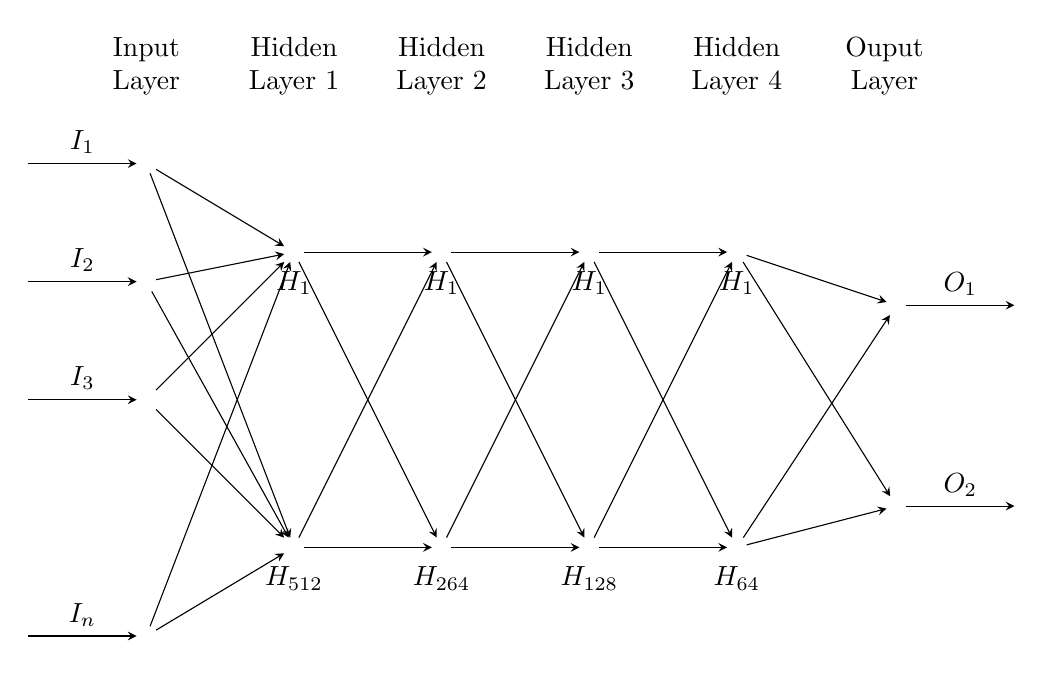
\begin{tikzpicture}[x=1.5cm, y=1.5cm, >=stealth]

\foreach \m/\l [count=\y] in {1,2,3,missing,4}
  \node [every neuron/.try, neuron \m/.try] (input-\m) at (0,2.5-\y) {};

\foreach \m [count=\y] in {1,missing,2}
  \node [every neuron/.try, neuron \m/.try ] (1-hidden-\m) at (1.25,2-\y*1.25) {};

\foreach \m [count=\y] in {1,missing,2}
  \node [every neuron/.try, neuron \m/.try ] (2-hidden-\m) at (2.5,2-\y*1.25) {};
  
 \foreach \m [count=\y] in {1,missing,2}
  \node [every neuron/.try, neuron \m/.try ] (3-hidden-\m) at (3.75,2-\y*1.25) {};

\foreach \m [count=\y] in {1,missing,2}
  \node [every neuron/.try, neuron \m/.try ] (4-hidden-\m) at (5,2-\y*1.25) {};
  
  
\foreach \m [count=\y] in {1,2}
  \node [every neuron/.try, neuron \m/.try ] (output-\m) at (6.35,2-\y*1.7) {};

\foreach \l [count=\i] in {1,2,3,n}
  \draw [<-] (input-\i) -- ++(-1,0)
    node [above, midway] {$I_\l$};

\foreach \l [count=\i] in {1,512}
  \node [below] at (1-hidden-\i.south) {$H_{\l}$};
  
  \foreach \l [count=\i] in {1,264}
  \node [below] at (2-hidden-\i.south) {$H_{\l}$};

\foreach \l [count=\i] in {1,128}
  \node [below] at (3-hidden-\i.south) {$H_{\l}$};

\foreach \l [count=\i] in {1,64}
  \node [below] at (4-hidden-\i.south) {$H_{\l}$};
  
\foreach \l [count=\i] in {1,...,2}
  \draw [->] (output-\i) -- ++(1,0)
    node [above, midway] {$O_\l$};

\foreach \i in {1,...,4}
  \foreach \j in {1,...,2}
    \draw [->] (input-\i) -- (1-hidden-\j);

\foreach \i in {1,...,2}
  \foreach \j in {1,...,2}
    \draw [->] (1-hidden-\i) -- (2-hidden-\j);

\foreach \i in {1,...,2}
  \foreach \j in {1,...,2}
    \draw [->] (2-hidden-\i) -- (3-hidden-\j);

\foreach \i in {1,...,2}
  \foreach \j in {1,...,2}
    \draw [->] (3-hidden-\i) -- (4-hidden-\j);

    
\foreach \i in {1,...,2}
  \foreach \j in {1,...,2}
    \draw [->] (4-hidden-\i) -- (output-\j);

\foreach \l [count=\x from 0] in {Input\\Layer, Hidden\\Layer 1, Hidden\\Layer 2, Hidden\\Layer 3, Hidden\\Layer 4, Ouput\\Layer}
  \node [align=center, above] at (\x*1.25,2) {\l};

\end{tikzpicture}
\caption{Fully connected αρχιτεκτονική}
\label{fig:FC_Arch}
\end{figure}


\bigskip
\subsection{Συνελικτική αρχιτεκτονική}

Υστερα από τα πειράματα που πραγματοποιήθηκαν σε πλήρως διασυνδεδεμένες αρχιτεκτονικές, ακολούθησε η δημιουργία και ο πειραματισμός με συνελικτικές δομές νευρωνικών δικτύων. Τα συνελικτικά νευρωνικά δίκτυα έχουν αναπτυχθεί σημαντικά τα τελευταία χρόνια λόγω της ικανότητάς τους να αναλύουν χωρική πληροφορία. Όσον αφορά την αρχιτεκτονική του συνελικτικού δικτύου, αποτελείται από 6 $1-D$ συνελικτικά επίπεδα με $32,32,64,64,128,128$ φίλτρα αντίστοιχα, με συνάρτηση ενεργοποίησης ReLu, όπου κάθε φίλτρο αποτελείται από ένα παράθυρο $3 \times 3$ , με κάθε συνελικτικό φίλτρο να ακολουθείται από ένα επίπεδο υποδειγματοληψίας που ονομάζεται \textit{Max Pooling}, με μέγεθος παραθύρου $3 \times 3$. 

\medskip
\begin{figure}[h]
  \centering
  \includegraphics[scale=0.65]{images/maxpool.png}
  \caption{Max Pooling}
  \label{fig:maxpool}
\end{figure}

\medskip
Κατά τη διαδικασία max pooling, από κάθε παράθυρο επιλέγεται η μέγιστη τιμή ως τιμη ως τιμή αντιπρόσωπος για το επόμενο επίπεδο. Με αυτό τον τρόπο επιτυγχάνεται μείωση της διαστασιμότητας του δικτύου ενώ παράλληλα πραγματοποιείται περιορισμός του θορύβου, καθώς οι θορυβώδεις τιμές απορρίπτονται. Στο τέλος του 6ου συνελικτικού επιπέδου εντοπίζεται ένα επίπεδο εξομάλυνσης (\textit{flatten layer}), που μετατρέπει την έξοδο σε ένα διάνυσμα στήλης. Στη συνέχεια, η έξοδος αυτή τροφοδοτείται σε ένα πλήρως διασυνδεδεμένο νευρωνικό δίκτυο με δύο επίπεδα, με $128$ νευρώνες το πρώτο και με $2$ νευρώνες το δεύτερο, που αποτελεί και το επίπεδο εξόδου.

\medskip
\begin{figure}[h]
  \centering
  \includegraphics[scale=0.8]{images/flatten.png}
  \caption{Flattening}
  \label{fig:flatten}
\end{figure}
\clearemptydoublepage

\chapter{Αποτελέσματα}\label{ch:chap4}
%!TEX root = ../main.tex
\setlength\belowcaptionskip{-1.5ex}

Στο κεφάλαιο \ref{ch:chap3} παρουσιάστηκε αναλυτικά η υλοποίηση της διπλωματικής εργασίας, απο την προεπεξεργασία και τροποποίηση των δεδομένων εως την παρουσίαση των αρχιτεκτονικών νευρωνικών δικτύων που χρησιμοποιήθηκαν. Σε αυτό το κεφάλαιο θα παρουσιαστούν τα αποτελέσματα και οι προβλέψεις των νευρωνικών δικτύων και θα πραγματοποιηθεί μια σύγκριση με αλλα υπάρχοντα μοντέλα πρόβλεψης αλληλεπιδράσεων πρωτεϊνών, αφού πρώτα ορισθούν όλες οι μετρικές αξιολόγησης των μοντέλων.


\section{Αποτελέσματα Εκπαίδευσης}

Προκειμένου να αξιολογήσουμε τα αποτελέσματα εκπαίδευσης, πρέπει να καθοριστεί το σύνολο των δεδομένων εκπαίδευσης με βάση το οποίο θα πραγματοποιηθεί η εκπαίδευση. Καθώς τα δεδομένα μας τροποποιήθηκαν από δύο αλγορίθμους, η λογική προσέγγιση θα ήταν η σύγκριση των αποτελεσμάτων εκπαίδευσης για τα δύο σύνολα και η επιλογή του συνόλου που αποδίδει καλύτερα. Ωστόσο, παρατηρώντας το περιεχόμενο των τιμών των δύο συνόλων ύστερα από την επεξεργασία, συμπεραίνουμε ότι έχουν παρόμοιες (σχεδόν πανομοιότυπες) εγγραφές, γεγονός που επιβεβαιώθηκε υπολογίζοντας την απόσταση \textit{Frobenius} των δύο μητρώων μέσω του τύπου: 

{\Large
$ dist(\textbf{A},\textbf{B}) =\sqrt{ \sum_{i=1}^{I}\sum_{j=1}^{J}( a_{ij} - b_{ij} )^2 } \approx 0$ }

\medskip
Επομένως, θα μπορούσαμε να επιλέξουμε ένα από τα δύο σύνολα εκπαίδευσης τυχαία για την εκπαίδευση/αξιολόγηση των μοντέλων μας. Ακόμη, παρατηρώντας τους χρόνους σύγκλισης των δύο αλγορίθμων, καταλήγουμε στη χρήση του συνόλου εκπαίδευσης που προέκυψε μέσω τανυστικής αποδόμησης για την εκπαίδευση των μοντέλων μας, καθώς η διαφορά στην ταχύτητα σύγκλισης καθιστά απαγορευτική την εκτέλεση της παραγοντοποίησης μητρώου μέσω SGD σε σχέση με την τανηστική αποδόμηση. 

\medskip
\begingroup
\centering
\newcommand\T{\rule{0pt}{3.0ex}} % Top strut
\newcommand\B{\rule[-2.0ex]{0pt}{0pt}} % Bottom strut
\begin{tabularx}{1\textwidth} { 
  | >{\centering\arraybackslash}X 
  | >{\centering\arraybackslash}X | }
 \hline
 \multicolumn{2}{|c|}{\textbf{Χρόνοι Σύγκλισης Μεθόδων}} \T\B \\
 \hline
 \textbf{Μέθοδος}\T\B & \textbf{Χρόνος (σε s)}\T\B \\
 \hline
 \textbf{Παραγοντοποίηση μητρώου μέσω SGD}\T\B & 1895.38\T\B \\
 \hline
 \textbf{CP αποδόμηση}\T\B & \textbf{26.04}\T\B \\
 \hline
\end{tabularx}
\captionof{table}{Χρόνοι σύγκλισης μεθόδων συμπλήρωσης μητρώων} 
\label{convtime}
\endgroup

\medskip
Όσον αφορά τα χρονικά αποτελέσματα της εκπαίδευσης, εμπειρικά παρατηρείται ότι η εκπαίδευση των πλήρως διασυνδεδεμένων επιπέδων ενός νευρωνικού δικτύου πραγματοποιείται πολύ πιο γρήγορα απ' ότι στην περίπτωση των συνελικτικών επιπέδων,ενώ τα συνελικτικά επίπεδα απαιτούν περισσότερη μνήμη για την αποθήκευση των ενδιάμεσων παραγώγων. Στην περίπτωσή μας, καθώς τα αποτελέσματα που παρουσιάζονται στη συνέχεια προέκυψαν από επικυρωμένη διασταύρωση (cross-validation), παρουσιάζονται οι χρόνοι για την εκπαίδευση μιας πτυχής (1 fold), με τα αποτελέσματα να εμφανίζονται στον πίνακα \ref{traintime}. Όπως παρατηρούμε,η εκπαίδευση του πλήρως διασυνδεδεμένου δικτύου χρειάστηκε \textbf{30} λιγότερες εποχές από αυτήν του συνελικτικού δικτύου, ωστόσο λόγω της γρηγορότερης εκτέλεσης των εποχών του συνελικτικού η εκπαίδευση του χρειάστηκε σχεδόν τον ίδιο χρόνο ($\approx 20$ λεπτά). Αξίζει να παρατηρηθεί επίσης ότι κάθε εποχή του συνελικτικού μοντέλου ήταν \textbf{1.33} φορές πιο γρήγορη από την αντίστοιχη του πλήρως διασυνδεδεμένου. Η συνθήκη σύγκλισης ήταν ίδια και για τα δύο μοντέλα και θεωρούσαμε σύγκλιση όταν δεν παρατηρούταν μεταβολή μικρότερη από $\delta = 2\times 10^{-4}$ στο \textit{σφάλμα επικύρωσης} (\textit{validation loss}) για ένα διάστημα 10 εποχών. 

\medskip
\begingroup
\centering
\newcommand\T{\rule{0pt}{3.0ex}} % Top strut
\newcommand\B{\rule[-2.0ex]{0pt}{0pt}} % Bottom strut
\begin{tabularx}{1\textwidth} { 
  | >{\centering\arraybackslash}X 
  | >{\centering\arraybackslash}X 
  | >{\centering\arraybackslash}X |}
 \hline
 \multicolumn{3}{|c|}{\textbf{Χρόνοι Σύγκλισης Μοντέλων}} \T\B \\
 \hline
 \textbf{Μοντέλο}\T\B & \textbf{Εποχές (ανά εποχή)} \T\B & \textbf{Χρόνος (σε s)}\T\B \\
 \hline
 \textbf{Πλήρως Διασυνδεδεμένο}\T\B & 75 (16.82s)\T\B & 1220.61 (20.3 λεπτά)\T\B \\
 \hline
 \textbf{Συνελικτικό}\T\B & 105 (12.61s)\T\B & 1225.28 (20.4 λεπτά)\T\B \\
 \hline
\end{tabularx}
\captionof{table}{Χρόνοι σύγκλισης νευρωνικών δικτύων} 
\label{traintime}
\endgroup

\newpage
\medskip
Παρακάτω, παρουσιάζονται οι γραφικές ακρίβειας και απωλειών των νευρωνικών δικτύων. Καθώς τα αποτελέσματα που παρουσιάζονται στη συνέχεια προέκυψαν από επικυρωμένη διασταύρωση (cross-validation), επιλέξαμε να αποτυπώσουμε τις απώλειες και την ακρίβεια ενδεικτικά για μια από τις 10 \textit{πτυχές} (folds). Φαίνεται από τις γραφικές παραστάσεις ότι το πλήρως διασυνδεδεμένο δίκτυο συγκλίνει αρκετά γρήγορα (75 εποχές) και μαθαίνει αρκετά γρήγορα το σύνολο εκπαίδευσης, κάτι που φαίνεται από την γρήγορη αύξηση της ακρίβειας και την πτώση των απωλειών. Ωστόσο, οι καμπύλες για τα δεδομένα επικύρωσης συγκλίνουν πολύ γρήγορα σε μια τιμή και στη συνέχεια παρουσιάζουν μια ταλαντωτική συμπεριφορά γύρω από αυτή, γεγονός που για να αποφευχθεί μας οδήγησε στην εκπαίδευση του πλήρως διασυνδεδεμένου μοντέλου με πολύ μικρό ρυθμό μάθησης ($= 0.00001$). Αυτό δείχνει την μεγάλη ευαισθησία του πλήρως διασυνδεδεμένου δικτύου, ενώ ταυτόχρονα δεν γενικεύει σε μεγάλο βαθμό. Από την άλλη, το συνελικτικό νευρωνικό δίκτυο απαιτεί περισσότερες εποχές για να συγκλινει (105 εποχές), ωστόσο συγκλίνει με πιο ομαλό τρόπο ενω δεν δείχνει να παρουσιάζει την έντονη ταλαντωτική συμπεριφορά του πλήρως διασυνδεδεμένου δικτύου, γι' αυτό και χρησιμοποιήθηκε μεγαλύτερη τιμή για τον ρυθμό μάθησης ($= 0.0001$).

\begin{figure}[H]
  \centering
  \includegraphics[width=1\textwidth]{images/DNNacc.png}
  \caption{Ακρίβεια πλήρως διασυνδεδεμένου νευρωνικού δικτύου}
  \label{fig:DNNacc}
\end{figure}

\begin{figure}[H]
  \centering
  \includegraphics[width=1\textwidth]{images/DNNloss.png}
  \caption{Απώλειες πλήρως διασυνδεδεμένου νευρωνικού δικτύου}
  \label{fig:DNNloss}
\end{figure}

\begin{figure}[H]
  \centering
  \includegraphics[width=1\textwidth]{images/CNNacc.png}
  \caption{Ακρίβεια συνελικτικού νευρωνικού δικτύου}
  \label{fig:CNNacc}
\end{figure}

\begin{figure}[H]
  \centering
  \includegraphics[width=1\textwidth]{images/CNNloss.png}
  \caption{Απώλειες συνελικτικού νευρωνικού δικτύου}
  \label{fig:CNNloss}
\end{figure}

Στη συνέχεια θα αναφερθούμε στις μετρικές που χρησιμοποιήθηκαν για την αξιολόγηση των μοντέλων μας. Αρχικά, η αντικειμενική συνάρτηση με βάση την οποία βελτιστοποιήθηκαν τα μοντέλα μας ήταν η \textit{απώλεια δυαδικής διασταυρωμένης εντροπίας} (\textit{binary crossentropy loss}).

{\noindent \Large
\begin{equation}
   J(w)= \frac{1}{m} \sum_{i=1}^{m}[ y_{i}*\log{\sigma(w^{\textit{T}}x_{i})} + (1-y_i)*\log{(1-\sigma(w^{\textit{T}}x_{i}))} ]
\end{equation}}

Για την αξιολόγηση της απόδοσης των μοντέλων και τη σύγκριση των αποτελεσμάτων χρησιμοποιήθηκαν οι ακόλουθες μετρικές:

\textit{Sensitivity}: Μετρική που εκφράζει την ποσότητα των θετικών περιπτώσεων που κατηγοριοποιούνται σωστά. Αποτελεί την σημαντικότερη μετρική όταν η αποφυγή των \textit{false negatives} έχει την ύψιστη σημασία.

\textit{Specificity}: Αντίστοιχη μετρική με το sensitivity, εκφράζει την ποσότητα των αρνητικών περιπτώσεων που κατηγοριοποιούνται σωστά, σημαντικό όταν μας απασχολούν τα \textit{false positives}.

\textit{Precision}: Μετρική που εκφράζει την πιθανότητα μιας θετικής κατηγοριοποίησης να είναι σωστή σε σχέση με όλες τις θετικές περιπτώσεις.

\textit{Accuracy}: Η πιο διαδεδομένη μετρική, εκφράζει την πιθανότητα μια κατηγοριοποίηση να είναι σωστή, ωστόσο δεν είναι πάντοτε αξιόπιστη στην περίπτωση δεδομένων που παρουσιάζουν \textit{ανισσοροπία} (\textit{imbalanced data sets}).

\textit{F1-score}: Αποτελεί τον αρμονικό μέσο των sensitivity και recall και αποτελεί ένα μέτρο αξιολόγησης της αποδοτικότητας ενός κατηγοριοποιητή, ωστόσο δεν λαμβάνει υπόψιν τις περιπτώσεις των \textit{true negatives}, εστιάζοντας κυρίως στις θετικές κατηγοριοποιήσεις.

\textit{MCC}: Γνωστή ως \textit{Matthew's Correlation Coefficient}, είναι ένα μέτρο συσχέτισης μεταξύ της πραγματικής τιμής και της πρόβλεψης. Λαμβάνει τιμές από $-1 - 1$, με το 0 να δηλώνει ότι οι προβλέψεις γίνονται τυχαία.

\medskip
\begingroup
\centering
\newcommand\T{\rule{0pt}{3.0ex}} % Top strut
\newcommand\B{\rule[-1.6ex]{0pt}{0pt}} % Bottom strut
\begin{tabularx}{1\textwidth} { 
  | >{\raggedright\arraybackslash}X 
   >{\centering\arraybackslash}X
   >{\raggedleft\arraybackslash}X | }
 \hline
 \multicolumn{3}{|c|}{\textbf{Μετρικές απόδοσης δυαδικής κατηγοριοποίησης}} \T\B \\
 \hline
 \textbf{Μετρική}\T\B & \textbf{Τύπος}\T\B & \textbf{Εύρος τιμών} \T\B \\
 \hline
 Sensitivity \T\B & {\Large$\frac{\textit{TP}}{\textit{TP+FN}}$ \T\B} & $[0,1]$\T\B \\
 \hline
 Specificity \T\B & {\Large$\frac{\textit{TN}}{\textit{TN+FP}}$ \T\B} & $[0,1]$\T\B \\
 \hline
 Precision \T\B & {\Large$\frac{\textit{TP}}{\textit{TP+FP}}$ \T\B} & $[0,1]$\T\B \\
 \hline
 Accuracy \T\B & {\Large$\frac{\textit{TP+TN}}{\textit{TP+TN+FP+FN}}$ \T\B} & $[0,1]$\T\B \\
 \hline
 F1 \T\B & {\Large$\frac{\textit{2TP}}{\textit{2TP+FP+FN}}$ \T\B} & $[0,1]$\T\B \\
 \hline
 MCC \T\B & {\Large $\frac{\textit{TP x TN - FP x FN}}{\sqrt{(\textit{TP}+\textit{FP}) (\textit{TP}+\textit{FN}) (\textit{TN}+\textit{FP}) (\textit{TN}+\textit{FN})}}$}\T\B & $[-1,1]$\T\B \\
 \hline
\end{tabularx}
\captionof{table}{Μετρικές απόδοσης δυαδικής κατηγοριοποίησης} 
\label{binarymetrics}
\endgroup

\medskip
Στον πίνακα \ref{binarymetrics} παρουσιάζονται οι μαθηματικοί τύποι που ορίζουν τις παραπάνω μετρικές. Ως \textit{true positive} (\textit{TP}) ορίζεται μια θετική περίπτωση που κατηγοριοποιείται ως θετική, ως \textit{false positive} (\textit{FP}) μια αρνητική περίπτωση που κατηγοριοποιείται ως θετική, ως \textit{true negative} (\textit{TN}) μια αρνητική περίπτωση που κατηγοριοποιείται ως αρνητική ενώ ως \textit{false negative} (\textit{FP}) μια αρνητική περίπτωση που κατηγοριοποιείται ως θετική.

\medskip
Εχοντας ορίσει τις μετρικές στον πίνακα \ref{binarymetrics}, προχωράμε στην εισαγωγή μερικών ακόμη εννοιών για την περαιτέρω κατανόηση των αποτελεσμάτων μας. Η πρώτη έννοια στην οποία θα αναφερθούμε είναι η \textit{καμπύλη AUC-ROC} (\textit{Area Under Curve - Reciever Operation Characteristics}). Η καμπύλη ROC αποτελεί μια μετρική που χρησιμοποιείται σε προβλήματα δυαδικής κατηγοριοποίησης προκειμένου να αξιολογηθεί η ποιότητα της εξόδου του κατηγοριοποιητή. Πρόκειται για μια καμπύλη πιθανότητας για διαφορετικές κατηγορίες, που εκφράζει την ικανότητα του μοντέλου να ξεχωρίσει τις δεδομένες κατηγορίες ως προς τις πιθανότητες πρόβλεψης. Στην εικόνα \ref{fig:ROC} φαίνεται μια τυπική καμπύλη ROC. Στον άξονα X υπάρχει ο ρυθμός \textit{False Positive}, δηλαδή την πιθανότητα μια αρνητική πρόβλεψη να είναι θετική, ενώ στον άξονα Y εχουμε τον ρυθμό \textit{True Positive}, δηλαδή την πιθανότητα μια θετική πρόβλεψη να είναι θετική. Εναλλακτικά, ο ρυθμός \textit{False Positive} αντιστοιχεί στην τιμή $1$-Specificity ενώ ο ρυθμός \textit{True Positive} αντιστοιχεί στην τιμή του Sensitivity.

\begin{figure}[H]
  \centering
  \includegraphics[width=1\textwidth]{images/ROC.jpg}
  \caption{Τυπική Καμπύλη ROC}
  \label{fig:ROC}
\end{figure}

\smallskip
Σχετικά με το περιεχόμενο της εικόνας \ref{fig:ROC}, ενα μοντέλο που προβλέπει τυχαία παρουσιάζει καμπύλη ROC που θα μοιάζει με την διαγώνια γκρι γραμμή και δεν έχει ικανότητα διάκρισης. Αντίθετα, όσο απομακρύνεται η καμπύλη από την διαγώνια γραμμή, τόσο καλύτερο είναι το μοντέλο στο να ξεχωρίζει τις θετικές περιπτώσεις από τις αρνητικές. Με βάση την παραπάνω καμπύλη, μπορούμε να εξάγουμε ορισμένες χρήσιμες μετρικές, όπως το σκορ \textit{AUC}. Οπως αναφέρει και το όνομα του, το AUC υπολογίζεται ως το εμβαδόν που βρίσκεται κάτω από την καμπύλη ROC και έχει αρκετές ερμηνείες. Συνοπτικά, είναι "η πιθανότητα ο κατηγοριοποιητής να κατατάξει ένα τυχαίο θετικό δείγμα υψηλότερα από ένα τυχαίο αρνητικό δείγμα" \cite{Hand2009MeasuringCP}. Το σκόρ AUC για έναν κατηγοριοποιητή που κάνει τυχαίες προβλέψεις (εμβαδόν κάτω από την γκρι διαγώνιο) θα είναι $0.5$, ενώ όσο αυξάνεται πλησιάζοντας την μονάδα δηλώνει και καλύτερη ικανότητα πρόβλεψης. Παρακάτω παρατίθενται οι καμπύλες AUC-ROC για κάθε μοντέλο που αναπτύξαμε, με την επιπλέον προσθήκη όπου θεωρούμε διαδοχικά κάθε κατηγορία ως την "θετική" κατηγορία.

\begin{figure}[H]
  \centering
  \includegraphics[width=1\textwidth]{images/DNNROC.png}
  \caption{Καμπύλη ROC πλήρως διασυνδεδεμένου νευρωνικού δικτύου}
  \label{fig:DNNROC}
\end{figure}

\begin{figure}[H]
  \centering
  \includegraphics[width=1\textwidth]{images/CNNROC.png}
  \caption{Καμπύλη ROC συνελικτικού νευρωνικού δικτύου}
  \label{fig:CNNROC}
\end{figure}

Από τα αποτελέσματα παρατηρούμε ότι και οι δύο αρχιτεκτονικές παρέχουν αρκετά ικανοποιητικά αποτελέσματα όσον αφορά τις προβλέψεις. Συγκεκριμένα, και για τις δύο αρχιτεκτονικές υπολογίζουμε: \newline$AUC_{DNN} = 0.8148$ και $AUC_{CNN} = 0.8121$. Οι τιμές βρίσκονται αρκετά κοντά μεταξύ τους για να μπορούμε να ξεχωρίσουμε κάποια αρχιτεκτονική,απλώς παρατηρούμε ότι η πλήρως διασυνδεδεμένη αρχιτεκτονική αποδίδει ελαφρώς καλύτερα από την συνελικτική όσον αφορά τη συγκεκριμένη μετρική.

Άλλη μια γραφική που μας βοηθάει στην κατανόηση της αποδοτικότητας των μοντέλων μας είναι η \textit{καμπύλη ακρίβειας ανάκλησης} (\textit{Precision Recall curve}). Η διαφορά με την καμπύλη ROC έγκειται στο γεγονός ότι η καμπύλη ακρίβειας ανάκλησης εστιάζει στην κατηγορία που ορίζεται ως κατηγορία μειονότητας, δεν λαμβάνει υπόψιν τις αρνητικές κατηγοριοποιήσεις και μας παρέχει χρήσιμη πληροφορία στην περίπτωση που δουλεύουμε με \textit{ανισόρροπα}(\textit{imbalanced}) σύνολα εκπαίδευσης. Στον άξονα Y βρίσκεται το precision, που εκφράζει την πιθανότητα μιας θετικής σωστής κατηγοριοποίησης ως προς το σύνολο των θετικών περιπτώσεων, ενώ στον άξονα Χ το recall, που εκφράζει την πιθανότητα μιας θετικής κατηγοριοποίησης ως προς τον αριθμό των πιθανών θετικών κατηγοριοποιήσεων που θα μπορούσαν να συμβούν. Είναι επιθυμητό τα μοντέλα μας να έχουν ταυτόχρονα υψηλή ακρίβεια και υψηλή ανάκληση, ωστόσο στην πραγματικότητα υπάρχει ενα trade-off μεταξύ των δυο.

\begin{figure}[H]
  \centering
  \includegraphics[width=1\textwidth]{images/DNNPRC.png}
  \caption{Καμπύλη Precision Recall πλήρως διασυνδεδεμένου νευρωνικού δικτύου}
  \label{fig:DNNPRC}
\end{figure}

\begin{figure}[H]
  \centering
  \includegraphics[width=1\textwidth]{images/CNNPRC.png}
  \caption{Καμπύλη Precision Recall συνελικτικού νευρωνικού δικτύου}
  \label{fig:CNNPRC}
\end{figure}
Παρατηρούμε ότι και στην περίπτωση της καμπύλης ακρίβειας-ανάκλησης, το πλήρως διασυνδεδεμένο νευρωνικό δίκτυο έχει οριακά καλύτερα αποτελέσματα από το συνελικτικό νευρωνικό δίκτυο. Στην περίπτωσή μας, η καμπύλες που μας απασχολούν είναι κυρίως οι καμπύλες που αφορούν την κατηγορίας 1, δηλαδή αυτές που ορίζουν ως θετική περίπτωση την ύπαρξη αλληλεπίδρασης. 

Στα αποτελέσματα της δημοσίευσης \cite{Northey2017} με την οποία συγκρίνουμε τα αποτελέσματά μας, λόγω της ύπαρξης \textit{NaN} τιμών στα χαρακτηριστικά του αρχικού συνόλου δεδομένων (ιδίως στα χαρακτηριστικά \textit{Conservation Scores}), παρατίθενται από τους συγγραφείς της δημοσίευσης τα αποτελέσματα για διαφορετικές περιπτώσεις εγγραφών. Στον παρακάτω πίνακα για τα αποτελέσματα των νευρωνικών δικτύων και των random forests επιλέχθηκαν τα αποτελέσματα όπου λαμβάνονται υπόψιν όλα τα χαρακτηριστικά. Στην περίπτωση που οι τιμές των χαρακτηριστικών είναι μη-έγκυρες, για τα νευρωνικά δίκτυα επιλέχθηκε μια τιμή που βασίζεται στον μέσο όρο της κατανομής των δεδομένων, ενώ για τα random forests χρησιμοποιήθηκε η μέθοδος \textit{fractional instances}, κατά την οποία εγγραφές που περιέχουν ελλιπείς τιμές διαιρούνται σε πολλαπλές τιμές με διαφορετικά βάρη.

\medskip
\begingroup
\centering
\newcommand\T{\rule{0pt}{3.0ex}} % Top strut
\newcommand\B{\rule[-1.6ex]{0pt}{0pt}} % Bottom strut
\begin{tabularx}{1\textwidth} { 
  |>{\raggedright\arraybackslash}X 
   >{\centering\arraybackslash}X
   >{\centering\arraybackslash}X
   >{\centering\arraybackslash}X
   >{\centering\arraybackslash}X
   >{\centering\arraybackslash}X
   >{\centering\arraybackslash}X | }
 \hline
 \multicolumn{7}{|c|}{\textbf{Σύγκριση μεθόδων}} \T\B \\
 \hline
 \textbf{Method} \T\B & \textbf{ACC}\T\B & \textbf{PREC} \T\B & \textbf{SPEC} \T\B & \textbf{SENS} \T\B & \textbf{F} \T\B & \textbf{MCC} \T\B \\
 \hline
 Neural Network \cite{Northey2017}  \T\B & $0.735$ \T\B & $0.653$ \T\B & $0.892$ \T\B & $0.415$ \T\B & $0.507$ \T\B & $0.355$ \T\B \\
 \hline
 Random Forest \cite{Northey2017} \T\B & \textbf{0.760} \T\B & $0.679$ \T\B & \textbf{0.906} \T\B & $0.439$ \T\B & $0.533$ \T\B & $0.398$ \T\B \\
 \hline
 CP + Fully Connected NN \T\B & $0.756$ \T\B & $0.756$ \T\B & $0.756$ \T\B & $0.756$ \T\B & $0.756$ \T\B & $0.512$ \T\B \\
 \hline
 CP + Convolu\-tional NN \T\B & $0.758$ \T\B & \textbf{0.758} \T\B & $0.758$ \T\B & \textbf{0.758} \T\B & \textbf{0.758} \T\B & \textbf{0.516} \T\B \\
 \hline
\end{tabularx}
\captionof{table}{Αποτελέσματα - Σύγκριση Μεθόδων} 
\label{binarymetrics}
\endgroup

\medskip
Τα παραπάνω αποτελέσματα αποδεικνύουν την βελτίωση της απόδοσης του κατηγοριοποιητή μέσω της συμπλήρωσης των ελλειπών τιμών και της χρήσης νευρωνικών δικτύων. Ειδικότερα, λαμβάνοντας υπόψιν τα αποτελέσματα του καλύτερου μοντέλου μας (αποδόμηση τανυστών και συνελικτική δομή νευρωνικών δικτύων), ενώ η απόδοση των νευρωνικών δικτύων που αναπτύξαμε είναι παρόμοια με αυτή της δημοσίευσης \cite{Northey2017}, η σωστή κατηγοριοποίηση των κομματιών επιφανείας (αύξηση του sensitivity κατά \textbf{72.66}$\%$ σε σχέση με τα random forests και κατά \textbf{82.65}$\%$ σε σχέση με την αρχιτεκτονική νευρωνικών δικτύων) καθώς και η συνολική αποδοτικότητα του κατηγοριοποιητή μας είναι σημαντικά βελτιωμένη. Χρησιμοποιώντας τον MCC ως κύρια μετρική αξιολόγησης, όπως πραγματοποιείται και στην δημοσίευση των Northey et al. και καθώς θεωρείται η καλύτερη μετρική αξιολόγησης ενός δυαδικού κατηγοριοποιητή σε θέματα υπολογιστικής βιολογίας, πετύχαμε αύξηση κατά \textbf{29.65}$\%$ σε σχέση με την αρχιτεκτονική των random forests και κατά \textbf{45.35}$\%$ σε σχέση με την αρχιτεκτονική νευρωνικών δικτύων \cite{Northey2017}. 

\newpage
\section{Μελλοντικές Εξελίξεις}

Στην ενότητα αυτή παρουσιάζονται διάφορες ιδέες σχετικά με την επέκταση της παρούσας διπλωματικής. Αρχικά, η πιο απλή διαδικασία για την βελτίωση των αποτελεσμάτων προέρχεται από την εκπαίδευση των μοντέλων μηχανικής μάθησης με ολοένα και περισσότερα δεδομένα και η αξιολόγηση τους σε ανεξάρτητα σύνολα αξιολόγησης, επομένως ως πρώτο βήμα θα μπορούσαν να εξαχθούν νέα δεδομένα από την πρωτεϊνική βάση δεδομένων PDB και να κατασκευαστούν νέα σύνολα δεδομένων εκπαίδευσης και αξιολόγησης με πιο σύγχρονα δεδομένα.

\medskip
Παράλληλα, όσον αφορά το σύνολο των δεδομένων εκπαίδευσης, θα μπορούσαν να προστεθούν περισσότερα χαρακτηριστικά, τόσο δομικά όσο και ακολουθιακά, για την εξαγωγή επιπλέον πληροφορίας σχετικά με τις αλληλεπιδράσεις μεταξύ πρωτεϊνών. Μερικά χαρακτηριστικά που παρουσιάζουν θετικά αποτελέσματα είναι οι \textit{φυσικοχημικές} ιδιότητες των αμινοξέων (\textit{physicochemical properties of amino acids}) \cite{Xie2020} και το \textit{σκορ αταξίας} (\textit{disorder score}) \cite{Li2012}.

\medskip
Όσον αφορά την προεπεξεργασία των δεδομένων, οι μέθοδοι συμπλήρωσης μητρώου λειτουργούν ιδανικά με μεγάλες δομές δεδομένων, γεγονός που δεν συμβαίνει στην περίπτωσή μας όπου έχουμε μόνο 8 χαρακτηριστικά. Ωστόσο, η ήδη υπάρχουσα απόδοση των αλγορίθμων θα μπορούσε να συγκριθεί με διαφορετικές μεθόδους. Μια σκέψη περιλαμβάνει την αξιολόγηση της τανηστικής αποδόμησης με πειραματισμους όσον αφορά την τιμή των $\beta_k$ \ref{beta} κατά την εφαρμογή των μεθόδων μη γραμμικής συζηγούς παραγώγου (ncg). Αντίστοιχα, θα μπορούσε να ελεγχθεί η αύξηση της ταχύτητας σύγκλισης του αλγορίθμου παραγοντοποίησης μητρώου μέσω SGD εφόσον υλοποιηθεί με κατανεμημένο τρόπο μέσω της τροποποιημένης μορφής του SGD που ονομάζεται \textit{Stratified Stochastic Gradient Descent} (\textit{SSGD}) \cite{Gemulla2011}.
\clearemptysinglepage

\bibliography{references}
\bibliographystyle{ieeetr}
\clearemptysinglepage

\input{lastpage}

\end{document}
